%%%%%%%%%%%%%%%%%%%%%%%%%%%%%%%%%%%%%%%%%%%%%%%%%%%%%%%%%%%%%%%%%%%%%%%%%%%%%%%%%%%%%%%%%%
% DISSERTATION
% Research Group Databases and Information Systems
% University of Innsbruck
%%%%%%%%%%%%%%%%%%%%%%%%%%%%%%%%%%%%%%%%%%%%%%%%%%%%%%%%%%%%%%%%%%%%%%%%%%%%%%%%%%%%%%%%%%



% include file containing tex configurations
\documentclass[a4paper, openright, twoside, parskip, titlepage, cleardoublepage=plain]{scrbook}
\usepackage[utf8]{inputenc}
\usepackage{graphicx}
\usepackage[automark]{scrpage2}
\usepackage[hyphens]{url}
\usepackage[draft=false]{hyperref} % draft=true -> print version
\usepackage{tikz}
\usepackage[Sonny]{fncychap}
\usetikzlibrary{shapes.callouts} 
\usepackage{fancybox}
\usepackage{pdfpages}
\usepackage[boxed,linesnumbered]{algorithm2e}
\usepackage[center,loose]{subfigure}
\usepackage{listings}
\usepackage[color=green]{todonotes}
\usepackage{paralist}
\usepackage{amsmath}
\usepackage{setspace}
\usepackage{titlesec}
\usepackage{float}
\usepackage{tocbasic}
\usepackage{amssymb}
\usepackage{caption}
\usepackage[flushmargin]{footmisc}

% gap below (sub)figures
\newcommand{\goodgap}{%
\hspace{\subfigtopskip}%
\hspace{\subfigbottomskip}}

%footnote behaviour
\subfiglabelskip=5mm

% make main captions of figures centered, not hanging
\captionsetup{format=plain,justification=centerlast}


% make toc header koma font
\renewcommand{\contentsname}{\textsf{Contents}}

% \titlespacing{heading_class}{⟨left⟩}{⟨above⟩}{⟨below⟩}[⟨right⟩]
\titlespacing*{\subsection}{0mm}{5mm}{-4mm}
\titlespacing{\subsubsection}{0mm}{3mm}{-4mm}
\titlespacing{\section}{0mm}{5mm}{-2mm}
%\titlespacing{\subsection}{0pt}{2mm}{2mm}

% line stretch
\setstretch{1.0}

% separator for footnote
\setlength{\footnotesep}{3ex}

% line stretch within itemize elements
\setlength{\plitemsep}{3mm}

% prevent koma to stretch half empty pages
\raggedbottom

% define gap between algorithm box and caption of the algoirithm
\SetAlCapSkip{2ex}

% size of chapter headers for fncychap
\ChTitleVar{\bfseries\fontsize{60}{30}}
\ChNumVar{\huge}


% prevent latex from splitting up footnotes on two separate pages
\interfootnotelinepenalty=100000

% setup for hyperref package
\hypersetup{
	hypertexnames=false,
    linktocpage=true,
    colorlinks,
    breaklinks=true,
    linkcolor=black,
    citecolor=black,
    urlcolor=blue,
    linkbordercolor={1 1 1}, % set to white
    citebordercolor={1 1 1}, % set to white 
    pdftitle={title},
    pdfauthor={name},
    bookmarksopen=true
}

% list of figures also includes subfigure captions
\setcounter{lofdepth}{2}

% code for creating empty pages
% no headers on empty pages before new chapter
\makeatletter
\def\cleardoublepage{\clearpage\if@twoside \ifodd\c@page\else
    \hbox{}
    \thispagestyle{empty}
    \newpage
    \if@twocolumn\hbox{}\newpage\fi\fi\fi}
\makeatother \clearpage{\pagestyle{empty}\cleardoublepage}

% Verhindern von "Schusterjungen" und "Hurenkindern"
\clubpenalty = 10000
\widowpenalty = 10000
\displaywidowpenalty = 10000
\tolerance=500 %Zeilenumbruch


% specify margins for two-sided print
\oddsidemargin 2cm
\evensidemargin 1cm
\textwidth 13cm
\topmargin 0.2cm

%% define header format
\renewcommand{\chaptermark}[1]{\chead{#1}}
\renewcommand{\sectionmark}[1]{\cohead{\thesection\ #1}}
\automark[chapter]{section} 
\clearscrheadfoot
\lehead{\leftmark}
\rohead{\rightmark}
\lohead{}
\rehead{}
\cfoot{\pagemark}

\setheadsepline{.4pt} % line below head


%% TikZ-Callout
\newcommand{\tweet}[2]{
\vspace{-0.6cm}
\begin{center}
\begin{tikzpicture}[remember picture]
  \node[rectangle callout,draw, text width = 10cm, inner sep=0.3cm] {\texttt{#1} \vspace{2mm} \newline \hspace*{2mm} \footnotesize {#2}};
\end{tikzpicture} 
\end{center}
\vspace{-0.7cm}
}

% framed boxes
\newenvironment{fminipage}%
{\begin{Sbox}
\begin{minipage}}%
{\end{minipage}\end{Sbox}\shadowbox{\TheSbox}}


% listings configuration
\lstset{
  numbers=left, 
  showspaces=false,
  captionpos=b,
  breaklines=true
}



\usepackage{listings}
\usepackage{color}
\usepackage{amsmath}
\usepackage[utf8]{inputenc}
\usepackage{xcolor,colortbl}
\usepackage{hyperref}
\usepackage{enumitem}
\usepackage{longtable}

\definecolor{dkgreen}{rgb}{0,0,0.6}
\definecolor{gray}{rgb}{0.5,0.5,0.5}
\definecolor{mauve}{rgb}{0.58,0,0.82}

\lstset{frame=tb,
  language=Java,
  aboveskip=3mm,
  belowskip=3mm,
  captionpos=t,
  showstringspaces=false,
  columns=flexible,
  basicstyle={\small\ttfamily},
  numbers=none,
  numberstyle=\tiny\color{gray},
  keywordstyle=\color{blue},
  commentstyle=\color{blue},
  stringstyle=\color{mauve},
  breaklines=true,
  breakatwhitespace=true
  tabsize=3
}

\usepackage{booktabs}
\usepackage{epigraph}
\definecolor{LightCyan}{rgb}{0.88,1,1}
\usepackage{hyperref}

\DeclareOldFontCommand{\rm}{\normalfont\rmfamily}{\mathrm}
\DeclareOldFontCommand{\sf}{\normalfont\sffamily}{\mathsf}
\DeclareOldFontCommand{\tt}{\normalfont\ttfamily}{\mathtt}
\DeclareOldFontCommand{\bf}{\normalfont\bfseries}{\mathbf}
\DeclareOldFontCommand{\it}{\normalfont\itshape}{\mathit}
\DeclareOldFontCommand{\sl}{\normalfont\slshape}{\@nomath\sl}
\DeclareOldFontCommand{\sc}{\normalfont\scshape}{\@nomath\sc}

\begin{document}



\pagestyle{scrheadings}

%+++++++++++++++++++++++++++++++++++++++++++++++++++++++++++++++++++++++++++++++++++++++
% TITLEPAGE
%+++++++++++++++++++++++++++++++++++++++++++++++++++++++++++++++++++++++++++++++++++++++
\title{\vspace{10pt}%Mitochondrial DNA Data Analysis in the Era of Massive Parallel Sequencing
Scalable Data Analysis of Mitochondrial DNA in the Era of High-Throughput Data Generation
\\[40pt]}
\subject{\vspace{30pt}Dissertation}

\author{Dipl.-Ing. Hansi Wei\ss{}ensteiner\\[40pt]}
\publishers{submitted to the Faculty of Mathematics, Computer
Science and Physics of the University of Innsbruck\\[10pt]
in partial fulfillment of the requirements

for the degree of ``Doktor der technischen Wissenschaften''\\[60pt]

\normalsize{Advisor: Univ.-Prof. Dr. G\"unther Specht}\\[20pt]

\normalsize{Innsbruck, 2017}
}
\date{}


\maketitle
\cleardoublepage





%+++++++++++++++++++++++++++++++++++++++++++++++++++++++++++++++++++++++++++++++++++++++
% ABSTRACT
%+++++++++++++++++++++++++++++++++++++++++++++++++++++++++++++++++++++++++++++++++++++++
\pagenumbering{Roman}

\hspace*{7cm}
\thispagestyle{empty}
\section*{Abstract}
\phantomsection  
\addcontentsline{toc}{chapter}{Abstract}

Computational methods are progressively required for data reproducibility and quality control in Genetics. This is especially true for mitochondrial DNA (mtDNA), which is used in a variety of disciplines, from archeogenetics, population genetics, to forensic DNA fingerprinting as well as clinical disease association studies. New methods for data generation increase the sample output, as well as the data volume per sample, requiring sophisticated computational methods for quality control. The increased sample size also increases the risk for data contamination or sample mix up. This work describes algorithms and the implemented system that can be combined into a workflow to manage mtDNA data derived from high-throughput devices, like massive parallel sequencing data. One central aspect presented is the classification of mtDNA data to phylogenetic clusters, used for mtDNA quality control and for detection of contamination patterns. Subsequently all required computational steps from sequence alignment, mapping, mutation detection, annotation and quality control are presented. To process the data, advantage of parallel computing architectures is taken and covered within this work. In conclusion, based on the presented scalable system, contamination can be detected in massive parallel sequencing data and the publication of false and misleading results can be prevented.

%The present work thereby describes algorithms to classify mtDNA profiles of samples into phylogenetic clusters, by comparing the results in terms of accuracy and speed. While new forms of mitochondrial therapies (like the mitochondrial replacement therapy) will become more prominent in the near future, haplogroups will become more relevant and an accurate estimation of haplogroups becomes essential. In this regard haplogroup matching is already proposed. 

%To be able to compare haplogroups based on the mitochondrial profile from a DNA sequence, an alignment step is required, in order to detect the single nucleotide polymorphisms on single bases, as well as insertions or deletions of larger fragments. Different approaches to perform this task are described and an implementation of an hash-index based on k-mers and dynamic programming is presented. The approach is compared to different data structures like suffix arrays and FM-Index, the latter being widely used for Next-Generation Sequencing (NGS). 

%With the previously mentioned progress in data generation by NGS, features of the mtDNA can be researched in more depth, to learn the still poorly understood process of mutation propagation. Here a new concept of processing large amount of mtDNA data derived by massive parallel sequencing devices is presented, by taking advantage of parallel computing architectures based on the MapReduce paradigm. Combined with herein described maximum likelihood model as well as filter steps, the workflow provides new insights in low-level mutations, as the result of different sequences per cell or tissue (called heteroplasmy). In order to validate the approach, several similar pipelines were compared in terms of sensitivity, specificity and precision. 

%Finally the applications described within this work can all be merged into a workflow for detecting contamination in massive parallel sequencing studies. Thereby this approach is based on the concept of haplogroup detection from low-level mutations present in the sequencing data. Different approaches for contamination detection are described and the performance of the approach is evaluated based on the publicly available data-set from the 1000 Genome Consortium, providing 2,504 whole genome sequencing data (up to 4.2 Tbases per sample were generated). We could confirm sample contamination within this data-set, based on the presented approach.

%In conclusion this work presents different algorithms, and implementations that can be applied for a specific task or combined to a system for performing quality control on mtDNA data. mtDNA being present in whole genome-, whole exome sequencing or RNA-sequencing projects poses the means of an inexpensive and rapid quality control as proposed as part of this work.

\cleardoublepage
\thispagestyle{empty}
\hspace*{7cm}
\section*{Zusammenfassung}
Computergestützte Methoden nehmen eine zusehends wichtigere Rolle im Bereich der Genetik ein; hier spielen vor allem die Reproduzierbarkeit von Ergebnissen und Qualit\"atskontrolle eine gro{\ss}e Bedeutung. Dies gilt insbesondere für die Analyse mitochondriale DNA (mtDNA), welche in einer Vielzahl von Disziplinen von essenzieller Bedeutung ist: unter anderem um genetische Ereignisse in der Evolution zu rekonstruieren, in der Forensik zum identifizieren von Personen oder sterblichen \"Uberresten, sowie in klinischen Studien, in der Forschung und in Therapie-Ans\"atzen. Mit der steigende Anzahl von genetischen Daten, welche durch neue Hochdurchsatz-Methoden mit steigendem Datenvolumen in immer gr\"o{\ss}eren Studienkollektiven produziert werden, steigt auch die Fehlerwahrscheinlichkeit und erfordert neue Methoden zur Qualit\"atskontrolle. Die vorliegende Arbeit besch\"aftigt sich mit Algorithmen und Methoden für Sequenzalignment, Klassifizierung von mtDNA Daten, parallelem Ansätzen zum Mapping von mtDNA Sequenzdaten sowie Detektion und Annotation von Mutationen. Mit Hilfe phylogenetischer Cluster, Haplogruppen genannt, wird ein neues Verfahren zur Detektion von Kontaminationen in mtDNA Daten vorgestellt. Dadurch kann einer Ver\"offentlichung von falschen und irref\"uhrenden Ergebnissen vorgebeugt werden. 


%Die vorliegende Arbeit beschreibt zunächst Algorithmen zur Klassifizierung von Proben und deren mtDNA-Profilen in phylogenetische Cluster, so genannten Haplogruppen. Die resultierende Software wird mit existierenden Ansätzen, sowie mit verschiedene Distanzmetriken verglichen, welche Modelle der DNA Evolution berücksichtigen. Ergebnisse in Bezug auf Genauigkeit und Geschwindigkeit werden dargestellt. Durch neue mitochondriale Therapieformen (wie die mitochondriale Spende, Stichwort Drei-Eltern-Kind) welche in naher Zukunft vermehrt in den Vordergrund gerückt werden, gewinnen Haplogruppen zunehmend an Wichtigkeit und die Klassifizierung wird immer kritischer. Im speziellen Fall der mitochondrialen Spende wird ein Haplogruppen-Abgleich (Matching) zwischen Spenderin und Empfängerin angeraten, was die Wichtigkeit der hier vorgestellten Software unterstreicht.

%Damit Haplogruppen basierend auf dem mitochondrialen Profil aus einer DNA-Sequenz verglichen werden können, ist ein Ausrichtungsschritt (Alignment) erforderlich, um die Unterschiede zur Referenzsequenz festzustellen. Dabei wird der Basenaustausch auf einzelnen Basen sowie Insertionen oder Deletionen größerer Fragmente so ausgerichtet und annotiert, dass diese verglichen werden können. Verschiedene Ansätze zur Durchführung dieser Aufgabe werden beschrieben und eine Implementierung eines Hash-Index basierend auf n-grams und dynamischer Programmierung wird vorgestellt. Der Ansatz wird mit unterschiedlichen Datenstrukturen wie Suffix-Arrays und FM-Index verglichen, wobei letzterer für das Next-Generation-Sequenzierung (NGS) sehr stark verwendet wird.

%Mit dem technologischem Fortschritt bei der Datenerzeugung durch NGS können Merkmale der mtDNA eingehender erforscht werden, um den noch weitgehend ungeklärten Ursachen der Entstehung und Vermehrung (Propagierung) von Mutationen zu erforschen. Hierzu wird ein Konzept zur Verarbeitung großer Mengen von mtDNA-Daten präsentiert. Die durch sogenannte massive parallele Sequenzierungsgeräte erstellten Sequenzdaten werden dabei unter Nutzung von parallelen Rechenarchitekturen basierend auf dem MapReduce-Paradigma verarbeitet. Kombiniert mit dem in dieser Arbeit beschriebenen Maximum-Likelihood-Modell sowie Filterschritten bietet der entwickelte Workflow neue Einblicke in Low-Level-Mutationen. Diese sind das Ergebnis unterschiedlicher mtDNA Sequenzen pro Zelle oder Gewebe und werden Heteroplasmie genannt. Um die Methode zu validieren, wurden mehrere ähnliche Pipelines hinsichtlich Übereinstimmung, Spezifität und Präzision bei der Auswertung von Heteroplasmien verglichen.

%Schließlich können die beschriebenen Methoden zu einem Workflow zum Nachweis von Kontaminationen in massiven parallelen Sequenzierungsstudien zusammengeführt werden. Dabei fundiert dieser Ansatz auf dem Konzept der Haplogruppen-Detektion von geringen Heteroplasmie-Level, um die Vermischung von zwei Proben in den Sequenzierungsdaten zu detektieren. Unterschiedliche Ansätze zur Kontaminationserfassung werden beschrieben und die Performance der Methode auf der Grundlage des öffentlich verfügbaren Datensatzes des 1000 Genome Consortium ausgewertet, wobei 2.504 vollständige Genomsequenzierungsdaten (bis zu 4.2 Tbasen pro Probe) bereitgestellt wurden. Wir konnten die bekannte Probenkontamination innerhalb dieses Datensatzes anhand der vorgestellten Methode bestätigen und damit zeigen dass der Einsatz dieser Methode in zukünftigen Sequenzierprojekten angestrebt werden sollte.

%Zusammenfassend stellt diese Arbeit mehrere Algorithmen und Implementierungen vor, die für eine spezifische Fragestellung im Bereich der mitochondrialen DNA angewendet oder zu einem Workflow zur Analyse und Qualitätskontrollen von mtDNA-Daten kombiniert werden können. Die mitochondriale DNA, welche in Genom-, sowie Exom- oder RNA-Sequenzierungsprojekten enthalten ist, kann durch die hier vorgestellten Methoden zu einer kostengünstige und schnelle Qualitätskontrolle verwendet und ausgenützt werden.

\phantomsection  
\addcontentsline{toc}{chapter}{Zusammenfassung}


\cleardoublepage
\phantomsection
%+++++++++++++++++++++++++++++++++++++++++++++++++++++++++++++++++++++++++++++++++++++++
% ACKNOWLEDGEMENTS
%+++++++++++++++++++++++++++++++++++++++++++++++++++++++++++++++++++++++++++++++++++++++
\section*{Acknowledgements}
\phantomsection  


This present work would not have been possible without the support of Dr. Sebastian Sch\"onherr and Lukas Forer PhD, thanks guys! 

Further thanks go to Priv.-Doz. Dr.in Dipl.-Ing.in Anita Kloss-Brandst\"atter for inspiring me for working in the field of "mtDNA", Univ.-Prof. Dr. Florian Kronenberg, as supporting employer, besides my doctoral adviser Univ.-Prof. Dr. G\"unther Specht. Further thanks to Univ.-Prof. Dr. Antonio Salas Ellacuriaga for constant advice and his patience.

Further thank to all the current and former GENEPI members (especially Margot, Anita, Stefan, Bernd) as well as the current and former DBIS members (especially Dominic and Robert).

A big thank goes to my family, especially my mother, providing me the required energy by passing on the H5r mitochondrial genome. 

A very special "thank you" goes to Anna! 

I'm very grateful that this thesis was supported by a scholarship from the Autonomous Province of Bozen/Bolzano - Alto Adige / S\"udtirol - (Studienbeihilfe f\"ur postuniversit\"are Ausbildungen). 

 
%
\cleardoublepage

\phantomsection

\cleardoublepage
\thispagestyle{plain}
\subsection*{Eidesstattliche Erkl\"arung}

Ich erkl\"are hiermit an Eides statt durch meine eigenh\"andige Unterschrift, dass ich die vorliegende Arbeit selbst\"andig verfasst und keine anderen als die angegebenen Quellen und Hilfsmittel verwendet habe. Alle Stellen, die w\"ortlich oder inhaltlich den angegebenen Quellen entnommen wurden, sind als solche kenntlich gemacht.
Die vorliegende Arbeit wurde bisher in gleicher oder \"ahnlicher Form noch nicht als Magister-/Master-/Diplomarbeit/Dissertation eingereicht. 


\vspace*{3cm}

\begin{tabular}{ccc}
\hspace*{4cm} & \hspace*{4cm} & \hspace*{4cm}\\\cline{1-1}\cline{3-3} 
Datum & & Hansi Wei\ss{}ensteiner\\
\end{tabular}

\graphicspath{ {./images/} }
\phantomsection  
\addcontentsline{toc}{chapter}{Table of Contents}
\tableofcontents
\phantomsection
\cleardoublepage

\renewcommand{\contentsname}{\textsf{Contents}}

\pagenumbering{arabic}
\setcounter{page}{1}
\include{0_acknowledgmements}
\cleardoublepage
\chapter{Introduction}
\label{chapterIntro}
\section{Motivation}
Increasing data volumes in the field of genetics require sophisticated computational methods, since the bottleneck is no longer the data generation itself, but shifted notably towards the data analysis \cite{Forer2016}. The whole human genome with its size of over 3 billion positions can now be analyzed in short time with decreasing prices. Therefore the amount of data that has to be dealt with already increased and will so even more dramatically in future. Therefore, new algorithms and methods for data quality control (QC) are required, for increasing precision and recall to exceed currently available methods, in a scalable way. Misleading results can impact medical studies or forensic casework, where errors introduced by computational methods can have severe consequences. The focus of this work is on computational methods for reproducible QC of DNA from a small genome, contained in the mitochondria. Although its length contributes only to $0.0005\%$ to the complete human genome, high-throughput data is required to investigate processes still unclear, like the development of mutations and its fixation in cancer or processes on the mitochondrial DNA (further denoted as mtDNA) related with aging. This data generation makes it indispensable to process without scalable and reproducible pipelines. 
\\
\\
The human mitochondrial DNA, henceforth abbreviated as mtDNA, plays an important role in today's life-science and is of especial interest in the field of population genetics, forensics and clinical disease association studies. The mitochondrial DNA has some features (more to find in Chapter \ref{chap:BioFound}) that make it predestined for genealogists when it comes to creation of family trees but also helps forensics in identifying persons or victims even with degraded body remains, or clinicians to help investigating diseases, since bioenergetic aspects, where mitochondria are heavily involved, offer new opportunities for diagnosis and therapy \cite{Picard2016}.
The following issues and challenges need to be addressed in this context:
\begin{itemize}
\item 
Mitochondrial DNA can be classified into a natural grouping of sequence haplotypes; into so called haplogroups. These haplogroups play an important role in the area of phylogenetics, but also in data QC of mtDNA data. While the manual assignment of mtDNA profles to haplogroups is very time-consuming besides being error prone, the increase of data generated, require sophisticated automatic procedures to solve this task. Therefore an algorithm is required to assigning the closest haplogroup to mtDNA profiles based on a maximum parsimony tree present \cite{VanOven2009}. With classical sequencing devices the data generation of mtDNA profiles might seem straightforward, but it is also error prone. To determine and correct these data errors, methods are required to perform QC to highlight issues in mtDNA data. The growing sample sizes in various studies require methods with linear increase in computation time and memory consumption, to consider the increasing data. 
\item 
One of the most prominent problems in the field of bioinformatics is the alignment of sequences. The algorithms in this regard are known to have complexity of $\mathcal O(nm)$ where \textit{n} and \textit{m} represent the length of the sequences to be compared, leading to $\mathcal O(n^2)$ in both time and space. There exist optimization as well as data structures to face this problem, and might seem trivial for mtDNA with its size of less than $\sim$ 17kb \cite{Andrews1999}. However, in order to detect variants according the correct nomenclature, several rules need to be considered, sometimes contradicting, rendering it almost impossible to generate unambiguous alignments \cite{Bandelt2008}. Ambiguous alignments without assumptions from evolutionary perspectives, especially in low-complexity regions, can influence the haplogroup assignment, and could lead to misinterpretation of results.  
\item 
A further challenge for computational biologists and computer scientists is the establishment of next-generation sequencing (NGS) devices in the last years, producing literally big data. The management of such data is not feasible for relational databases, requiring new paradigms such as key-value based models like MapReduce \cite{Dean2008}. The mtDNA with it's small size is in contrast to the nuclear DNA a tiny genome sequence, but due to it's property, being present between 100 and several 1,000 fold per cell, it requires sequencing with high coverage. This exploitation of the massive parallel sequencing is required in order to get a deeper understanding in mitochondrial mutations. These mutations are often involved in diseases and poorly understood at this time \cite{Wallace2013}. Since the error rates of the new devices are higher than the former gold standard \cite{Wang2011}, additional QC-steps are required, to prevent the detection of false positive mutations. 

\end{itemize}

In this thesis, solutions to the drafted issues are proposed. Software tools, which can operate as stand-alone applications but that can also be merged to one pipeline for contamination detection in NGS studies, are presented. Thereby the detection of contamination is not limited to pure mtDNA sequencing projects. By taking advantage of  mtDNA sequences contained in whole genome sequencing or whole exome sequencing projects, benefit of this approach for contamination detection is proposed. It therefore represents a fast and straightforward method for quality control of massive parallel sequencing datasets prior to publication. Thereby mtDNA makes an intrinsic contamination control for whole genome sequencing projects available and highlights the merits of this underrated extra “chromosome” paired with computational methods. The scalable pipeline can handle large data sets of several hundred GBs as shown in the context of this work. 

\section{Preliminary Work}
\label{prelimWork}
This work is the continuation of an interdisciplinary cooperation between the group of Databases and Information Systems of the University of Innsbruck and the Department of Genetic Epidemiology at the Medical University of Innsbruck which started back in 2007 and led to my master's degree in computer science in 2008. Back then the focus was on the development of a database for genotype data (the blueprint of an organism, contained in each cell) and phenotype data (an organism's observed properties, such as the physical appearance like eye color or the body mass index, disease or behavior with the result published in BMC Bioinformatics \cite{Schoenherr2009}. This database was the foundation for the next project, which was to extend it for QC and further functionality to work with a special and very specific DNA from an organelle with its own genome, the mitochondrial genome. 
\\
Different methods for the generation of mtDNA data exist, as presented in section \ref{sec:dataGeneration}. While the data generation is getting increasingly more straightforward, the data management gets more complex. Checks for data quality are needed, to avoid the processing of false positive data, that could lead to misinterpretation of diseases, to wrong publications and conclusions or even to the arrest of innocent persons, just to show the severity these consequences can have in the different areas applied.
Therefore a short summary about this basic concept is presented here, that shows the mtDNA data management in a relational database. Since this system is based on a previous work by Sch\"onherr and Weissensteiner \cite{Schoenherr2009} from 2009, the database structure's concept is to store phenotypes in a key-value like schema (where a key has a value and a time-stamp), by implementing 3 different entities for each data-type $(STRING, INTEGER, DOUBLE)$.
\begin{figure}[ht]
\begin{center}
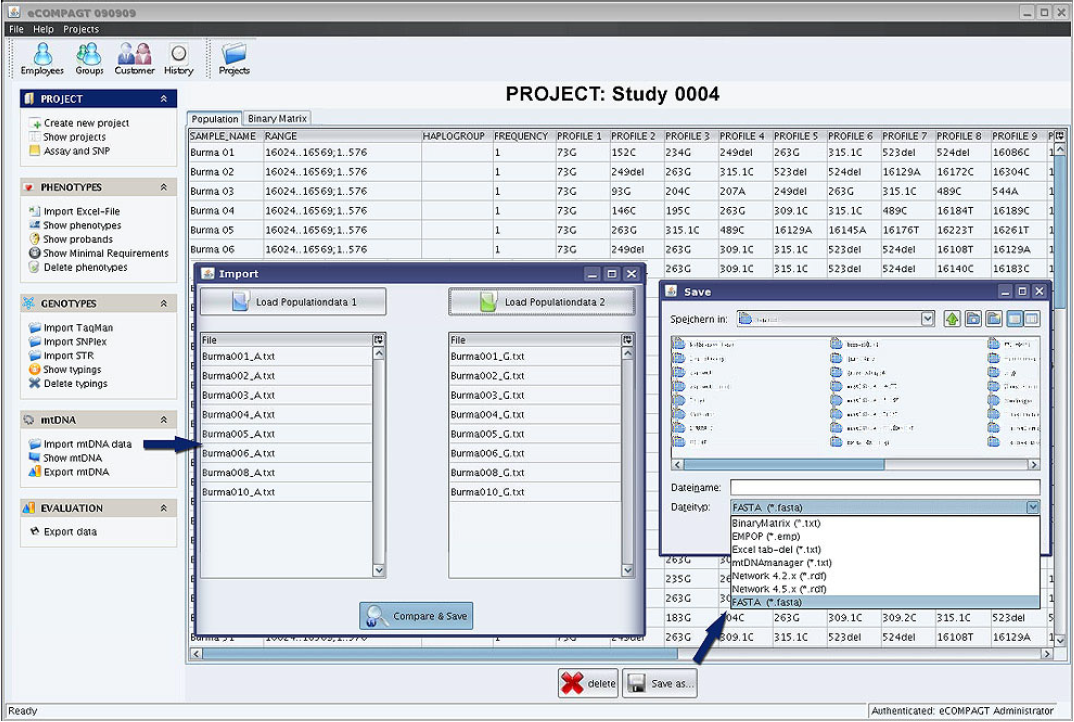
\includegraphics[scale=0.46]{ecompagt.png}
\caption[eCOMPAGTs User Interface]{eCOMPAGTs User Interface for mtDNA handling: the input data is checked for concordance, while several file exports are supported. Figure presented in Weissensteiner et al. \cite{Weissensteiner2010}}.
\label{fig:ecompagt}
\end{center}
\end{figure}
Both phenotypes and genotypes are stored in a previously IBM DB2 database, in an updated version also Oracle and MySQL relational database management systems are supported. When working with mtDNA data from sequencing devices, we integrated an workflow for the analysis in eCOMPAGT, to securely import, validate, store and export mtDNA profiles.  These can further be connected to phenotype data by using eCOMPAGT's combination and evaluation feature. Data import comprise data in EMPOP format \cite{Parson2007}, or from Sequencher/SeqScape mutation reports. Data Exports provide various formats for different applications: EMPOP as well as FASTA files, file for generation of phylogenetic networks in Network.exe\footnote{\url{fluxus-engineering.com}}  \cite{Bandelt1999}, mtdnaManager\cite{Lee2008}, as well as HaploGrep input files \cite{Kloss-Brandstatter2011,Weissensteiner2016a}. Figure \ref{fig:ecompagt} shows the graphical user interface of the database, based on Java Swing and SwingX. The workflow, as well as the underlying architecture are not further presented in this work, I refer to the publications by Sch\"onherr and Weissensteiner \cite{Schoenherr2009,Weissensteiner2010}. These articles build the groundwork of the subsequently research effort. One previously identified limitation of this system is addressed and solved in the the subsequenct Chapter \ref{chapterHaplogrep}, by presenting HaploGrep.

\section{Problem characterization}
\label{sect:ProblChar}
The aim of this work is to propose an information management system for mtDNA data. 
The most common input formats from Sanger based Sequencing, over genotyping data from MicroArrays to the Next-Generation Sequencing for mitochondrial DNA  are covered and merged into a management system for quality control. Sample contamination is still a severe problem, not only for anthropologists dealing with degraded mtDNA but for all types of areas dealing with mtDNA (forensics, medical genetics, population genetics). With new technologies, contamination detectable due to the high resolution of genomes, becomes a new issue in the lab, and requires control mechanisms in data post-processing. Therefore quality control based on the mitochondrial DNA haplogroups is essential for both Sanger Sequencing as well as for Next-Generation-Sequencing and will play a major role in this thesis. Within the next Chapter \ref{chap:BioFound} Biological Background, the basic features of mtDNA, as well as the data formats are presented. An already implemented database for mtDNA data were presented (Publications in BMC Bioinformatics \cite{Schoenherr2009}, \cite{Weissensteiner2010}) as drafted in \ref{prelimWork}, able to perform basic QC steps only.

The core purpose of this investigation was to build an information system for managing data from the often so called powerhouses of the cell, the mitochondria with their own mitochondrial DNA. Besides the initial database (see \ref{prelimWork}, several additional algorithms and frameworks which all can be connected to a pipeline and as a matter of fact are connected in Chapter \ref{chap:NGS} and Chapter \ref{chapterContamination} yield to high-quality mtDNA data. The herein developed JAVA based software solutions are abstracted in the next paragraphs and are presented in detail in the corresponding chapters.

Chapter \ref{chapterHaplogrep} describes the foundations of mitochondrial classification to haplogroups based on an XML tree. Several binary similarity and distance measures are evaluated and our solution HaploGrep is compared to related work. \\

Chapter \ref{chap:alignment} deals with the theoretical background as well as the JAVA implementation for aligning mitochondrial genome data efficiently as an extension to chapter \ref{chapterHaplogrep}, and are presented as part of the subsequent publication. As data volume increases with Next-Generation Sequencing, a MapReduce based approach is presented in chapter \ref{chap:NGS} to sequence the mitochondrial genome with a high coverage, resulting in computational intensive mapping of the short-reads to the reference sequence. 
\\
The resulting profiles yield insights in heteroplasmy levels and are an indication for data quality by applying an haplogroup discordance check presented in chapter \ref{chapterContamination}. Based on this check contamination not only in targeted mtDNA sequencing studies, but also in Whole Genome and Whole Exome Sequencing Projects can be detected. This approach is partly presented in Weissensteiner et al. \cite{Weissensteiner2016b} and is part of a work that is currently prepared for publication. Figure \ref{fig:figureBigPic} gives an overview of the chapters represented in this work and their relation as a schematic software stack.
\\ 
The chapter \ref{chap:conclusion} finally gives a summary of the different key aspects, shows strengths and limitations of our pipeline while Chapter \ref{outlook} gives an outlook of possible optimization and on future work.

\begin{figure}[ht]
\begin{center}
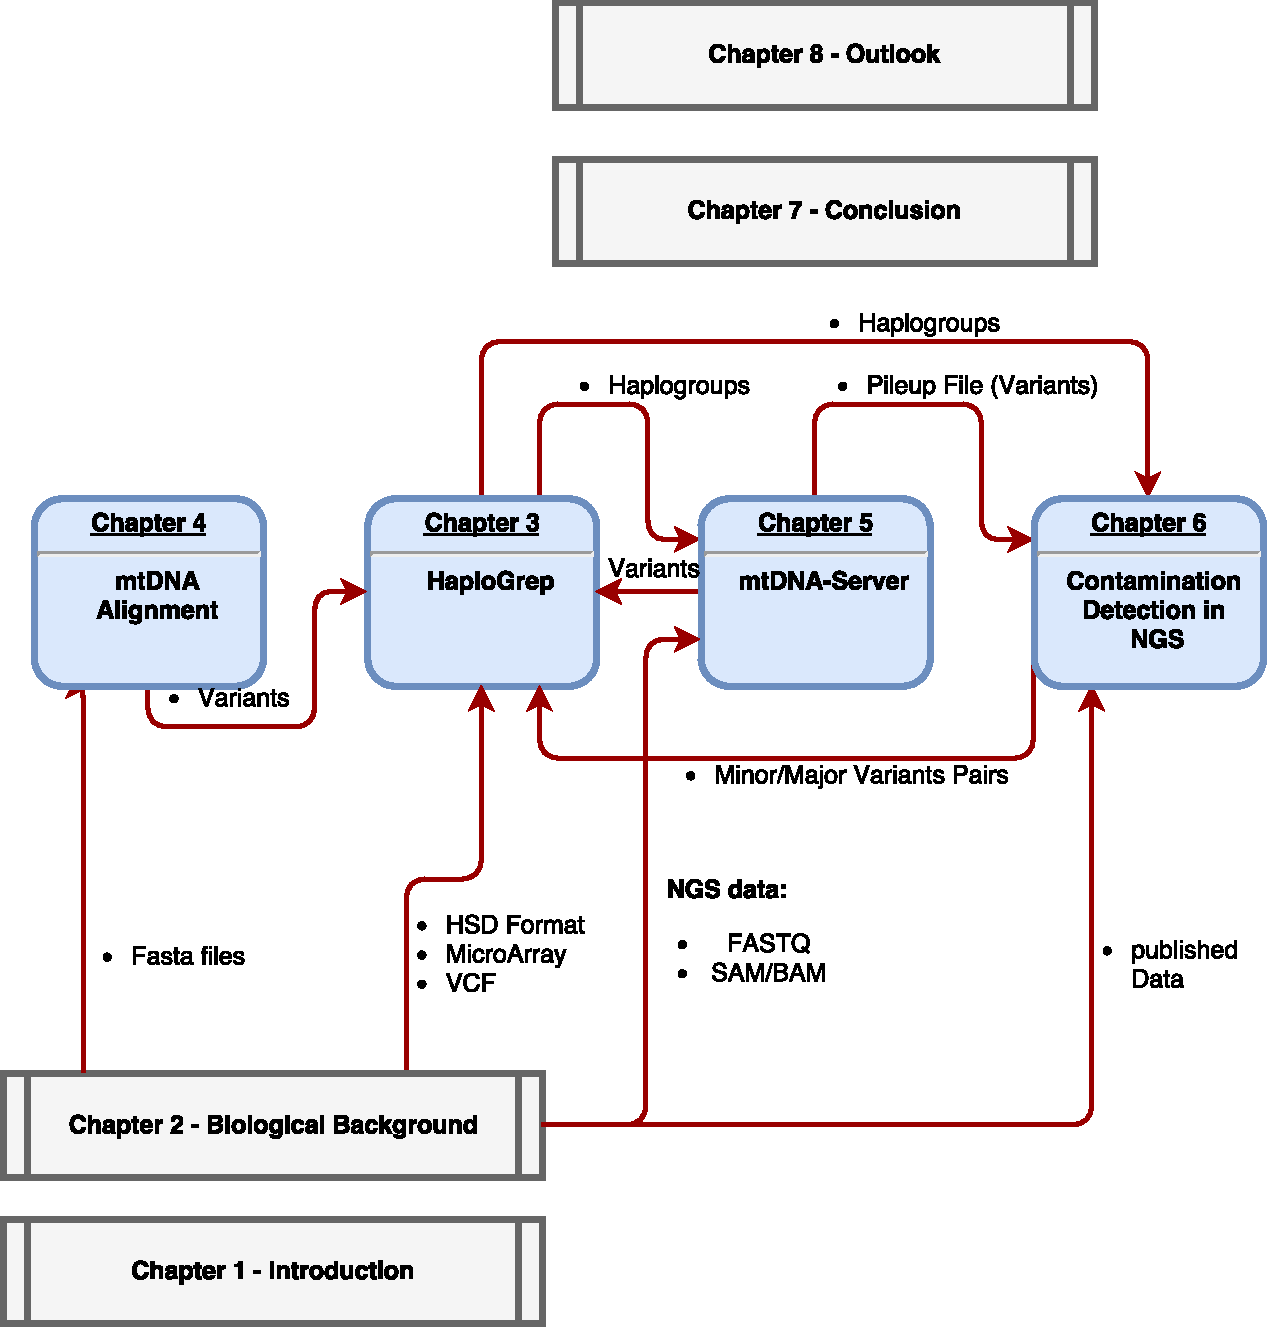
\includegraphics[scale=0.5]{BigPicture.pdf}
\caption[Representation of chapters]{Representation of chapters and their connection to a contamination detection method, covering various file formats }
\label{fig:figureBigPic}
\end{center}
\end{figure}

\section{Research Aims and Contribution}
Research demands collaboration. This work is largely the result of collaboration with computer scientists, programmers, database experts, biologists, mathematicians, medical doctors, medical technical assistants and many more. It is in fact interdisciplinary, as it is for genetics and genomics in general. Given the growing data generated with new sequencing devices, it is not feasible to process the data without a reproducible system, that takes the technical hurdles from the end user. Therefore the research aim is on providing sophisticated methods to the biologists, in such a manner that a problem can be solved by hiding the complexity from the user. Here it is mostly related with the handling of mtDNA data, where the end users have different background. The subsequent chapters represent some of the main work over several years of daily work with mtDNA data, highlighting the main contributions as drafted, resulting in several publications. 

The result presented in Chapter \ref{chapterHaplogrep} was published in Kloss-Brandst\"atter et al with shared first authorship in the journal Human Mutation \cite{Kloss-Brandstatter2011} and the successive extensions and optimizations were published in Weissensteiner et al presenting HaploGrep 2 in the 2016 Web Server Issue\footnote{\url{http://nar.oxfordjournals.org/content/44/W1.toc}} of Nucleic Acids Research\cite{Weissensteiner2016a}.

The work presented in Chapter \ref{chap:NGS} was also accepted in the 2016 Web Server Issue of Nucleic Acids Research in Weissensteiner et al \cite{Weissensteiner2016b} (acceptance quote of 31\%, see Editorial\footnote{\url{http://nar.oxfordjournals.org/content/44/W1/W1.full}}).

These published applications helped subsequent research questions, that led to further contributions in various publications (see Curriculum Vitae for full list of contributions), the most related with this work are the results in Summerer et al 2014 published in BMC Evolutionary Biology, \cite{Summerer2014} where we analyzed the mtDNA of 327 donors from Myanmar by considering the migration and generated phylogenetic trees identifying novel clusters. 

In a further work published in the Proceedings of the National Academy of Sciences \cite{Kehdy2015}, we analyzed the mtDNA data from 6,487 individuals, confirming the low native-american ancestry after european conquest, and shedding light on the African diaspora, where Brazil was a major destination.

The foundations for mtDNA-Server (Chapter \ref{chap:NGS} derived from two research projects: the MapReduce Framework Cloudgene \cite{Schonherr2012}, which we published in BMC Bioinformatics in 2012 and the Cancer Study of 28 individuals, where we compared different tissues in oral squamous cell carcinoma \cite{Kloss-Brandstatter2015}, by comparing Sanger based Sequencing to Next-Generation Sequencing, and showed that heteroplasmy detection down to the 1\% level is feasible with the new devices and the herein presented Apache Hadoop based approach. 

The further development of Cloudgene led to subsequent publication of Cloudflow in  2015 \cite{Forer2015} and 2016 \cite{Forer2016} respectively. Herein the Framework was extended not only to support Apache Hadoop with MapReduce but also Apache Spark pipelines. 

Several topics outside the mtDNA-field were also addressed in the recent years, leading to publications in the various peer-review journals like \textit{PLOS ONE} \cite{Weissensteiner2013} by describing SNPflow, a JAVA based application with an Ext-JS JavaScript user interface, an embedded Apache Tomcat server and MySQL-database for QC of genotype data derived by multiplex genotyping platforms. 

In the journal \textit{Atherosclerosis} we described a risk score for cardiovascular disease\cite{Lamina2014} implemented in JavaScript, and presented various works related to the relative telomere length \cite{Raschenberger2015assoc,Raschenberger2015dotelomeres}, in the German Chronic Kidney Disease (GCKD) study.

Lately, by modifying mtDNA-Server to work with different reference sequences, we were able to identify novel variants in a so far still unresolved highly repetitive region on the nuclear DNA, in the LPA gene, associated with cardiovascular disease \cite{Kronenberg2014}. The work is currently in press in the \textit{European Heart Journal} \cite{Coassin2017}. 


The work for the GCKD study lead to a membership of the consortium. As of February 2017 a membership in a consortium lead by the Max-Planck Institute for the Science of Human History was added.

Several conferences and workshops were attended in the last years (see CV), including venues in Qatar, USA, UK, Netherlands, Croatia, Germany and Austria, mostly in context of mtDNA data analysis. 


% \textit{2016}{H Weissensteiner et al. \textbf{mtDNA-Server: next-generation sequencing data analysis of human mitochondrial DNA in the cloud}, \textit{Nucleic Acids Research - Web Server Issue 2016}}
% \textit{2016}{H Weissensteiner et al. \textbf{HaploGrep 2: mitochondrial haplogroup classification in the era of high-throughput sequencing}, \textit{Nucleic Acids Research - Web Server Issue 2016}}
% \textit{2016}{L Forer et al. \textbf{Cloudflow-enabling faster biomedical pipelines with MapReduce and Spark}, \textit{Scalable Computing: Practice and Experience}}
% \textit{2015}{J Raschenberger et al. \textbf{Association of relative telomere length with cardiovascular disease in a large chronic kidney disease cohort: The GCKD study}, \textit{Atherosclerosis}}
% \textit{2015}{J Raschenberger et al. \textbf{Do telomeres have a higher plasticity than thought? Results from the German chronic kidney disease (GCKD) study as a high-risk population}, \textit{Experimental gerontology}}{}
% \textit{2015}{A Kloss-Brandst{\"a}tter et al. \textbf{Validation of Next-Generation Sequencing of Entire Mitochondrial Genomes and the Diversity of Mitochondrial DNA Mutations in Oral Squamous Cell Carcinoma}, \textit{PloS One}}
% \textit{2015}{FSG Kehdy et al. \textbf{Origin and dynamics of admixture in Brazilians and its effect on the pattern of deleterious mutations}, \textit{Proceedings of the National Academy of Sciences}}
% \textit{2015}{L Forer et al. \textbf{Cloudflow-A framework for MapReduce pipeline development in Biomedical Research}, \textit{Information and Communication Technology, Electronics and Microelectronics (MIPRO)}}
% \textit{2014}{ C Lamina et al. \textbf{Correlation between a positive family risk score and peripheral artery disease in one case-control and two population-based studies}, \textit{Atherosclerosis}}
% \textit{2014}{L Forer et al. \textbf{Delivering bioinformatics MapReduce applications in the cloud}, \textit{Information and Communication Technology, Electronics and Microelectronics (MIPRO)}}
% \textit{2014}{M Summerer et al. \textbf{Large-scale mitochondrial DNA analysis in Southeast Asia reveals evolutionary effects of cultural isolation in the multi-ethnic population of Myanmar}, \textit{BMC Evolutionary Biology}}
% \textit{2013}{ H Wei{\ss}ensteiner et al. \textbf{SNPflow: a lightweight application for the processing, storing and automatic quality checking of genotyping assays}, \textit{Plos One}}
% \textit{2012}{ S Sch\"onherr et al. \textbf{Cloudgene: A graphical execution platform for MapReduce programs on private and public clouds}, \textit{BMC Bioinformatics}}
% \textit{2012}{L Forer et al. \textbf{Cloud Computing}, \textit{Book Chapter: Computational Medicine}}
% \textit{2011}{S Sch\"onherr et al. \textbf{A feedback guided interface for elastic computing}, \textit{Grundlagen von Datenbanken}}
% \textit{2010}{A Kloss-Brandst{\"a}tter et al. \textbf{HaploGrep: a fast and reliable algorithm for automatic classification of mitochondrial DNA haplogroups}, \textit{Human mutation}}
% \textit{2010}{L Forer et al. \textbf{CONAN: copy number variation analysis software for genome-wide association studies}, \textit{BMC Bioinformatics}}{}
% \textit{2010}{H Wei{\ss}ensteiner et al. \textbf{eCOMPAGT integrates mtDNA: import, validation and export of mitochondrial DNA profiles for population genetics, tumour dynamics and genotype-phenotype association studies}, \textit{BMC Bioinformatics}}
% \textit{2009}{S Sch\"onherr et al. \textbf{eCOMPAGT - efficient combination and management of phenotypes and genotypes for genetic epidemiology}, \textit{BMC Bioinformatics}}

\cleardoublepage
\chapter{Biological Background} 
\label{chap:BioFound}
This chapter gives a short overview of the biological foundations, as a background for non-biologists from the view of a computer scientist, to understand the algorithms and applications presented in this thesis, by covering all relevant biological aspects in a simple manner. Due to the fact that the mitochondrial genome sequence is fully decoded since 1981 by Anderson \cite{Anderson1981} and corrected later in 1999 by Andrews et al. \cite{Andrews1999} to the revised Cambridge Reference Sequence (rCRS) with 16569 bases, its analysis has matured in the course of the past 20 years \cite{BandeltHansJurgenRichardsMartinMacaulay2006}. Since then the importance of mtDNA gained, now widely being used for population genetics, forensic DNA fingerprinting and clinical disease association studies \cite{Weissensteiner2010}. In this work the focus is on software tools for human evolution (haplogroups) and disease (haplogroups, heteroplasmy), at first sight appearing unrelated, but the evidence increases that the evolution of mtDNA can have a role in disease expression\cite{BandeltHansJurgenRichardsMartinMacaulay2006}. 

\section{Mitochondrial DNA}
Mitochondrial DNA, which is the data being managed in this thesis, is a sequence of 16.6 kilobases in length (kb), consisting of 4 nucleobases, namely Adenine (A),Cytosine (C), Guanine (G) and Thymine (T). The mitochondrial genome is most likely the result of an endosymbiotic process, indicated by the similarity to bacterial (prokaryotic) DNA \cite{Pittis2016}, being circular (see Figure \ref{fig:rcrs}), differing significantly from nuclear DNA (see Table \ref{tab:features}) and showing codons, that differ from the nuclear ones (see Table \ref{tbl:aac}. 
\begin{figure}[ht]
\begin{center}
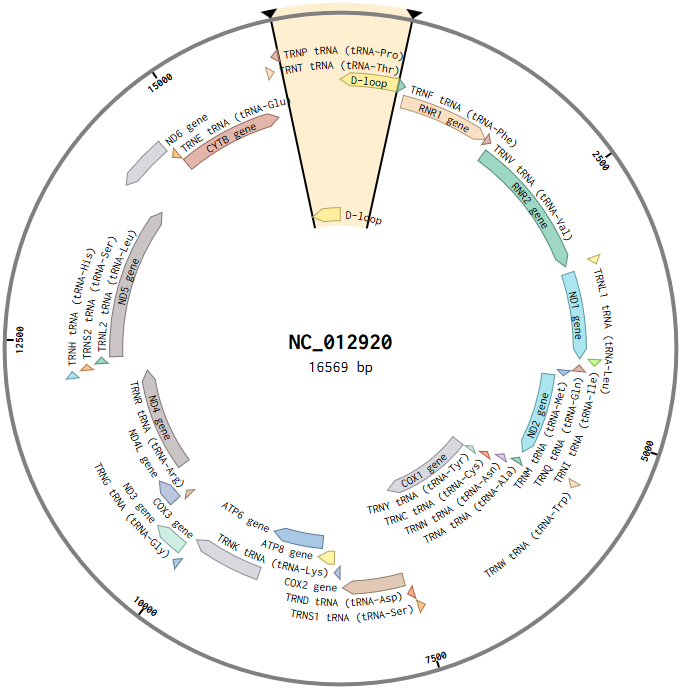
\includegraphics[scale=0.5]{rcrs.png}
\caption[Genomic organization of human mtDNA]{Genomic organization of human mtDNA. }
\label{fig:rcrs}
\end{center}
\end{figure}
It is a circular, double stranded molecule, whereat Cytosine binds to Guanine and Adenine to Thymine. One of the two strands is a guanosine-rich "`heavy"' strand (H-strand), the other a cytosine-rich "`light"'strand (L-strand). This is due to the fact that purines (Adenine and Guanine) are heavier than the pyrimidines (Thymine and Cytosine) due to their extra ring, see Figure \ref{fig:figureBases}.
\begin{figure}[ht]
\begin{center}
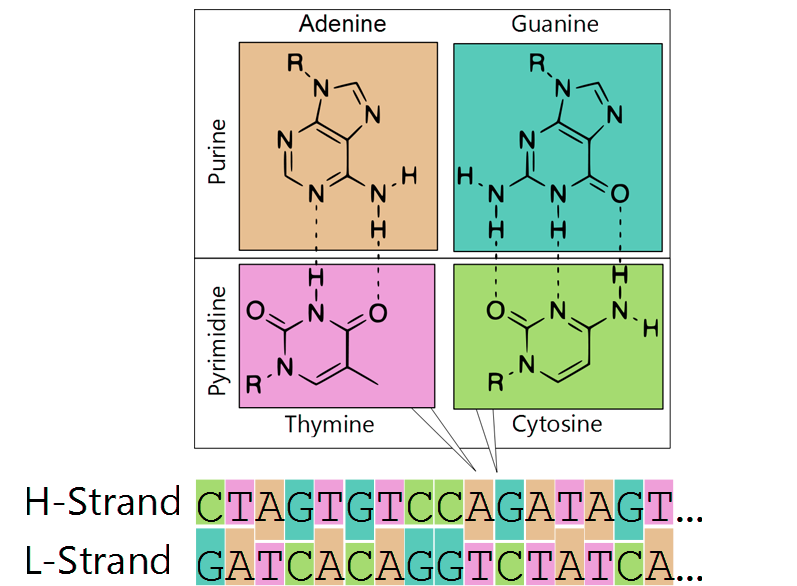
\includegraphics[scale=0.3]{bases2.png}
\caption[Nucleobases binding to a sequence]{Nucleobases binding to a sequence. For convenience only the L-strand is used as the reference sequence (here the first bases of the rCRS), since the H-strand is the complement that can be derived from this sequence.}
\label{fig:figureBases}
\end{center}
\end{figure}

The human mtDNA is numbered according to the light-strand, based on the original Cambridge Reference Sequence \cite{Anderson1981}. This reference sequence contained some major errors (10 substitution errors and a deletion), but to avoid confusion the authors of the revised CRS (rCRS) \cite{Andrews1999} kept the original light-strand numbering system by introducing a base N (for any) to keep the numbering with older analyses consistent. Behar et al. \cite{Behar2012} introduced an artificial new reference sequence, the so called Reconstructed Sapiens Reference Sequence (RSRS) \cite{Bandelt2013}, however being kept consistent with the numbering. This was not the case with the Genome Reference Consortium build 36 (NCBI Build 36.1 from March 2006)\footnote{\url{https://genome.ucsc.edu/FAQ/FAQreleases.html}} by using a Yoruba individual (YRI) sequence. Due to insertions and deletions (indels) this reference led and still leads to confusion among researchers. The reference was removed\footnote{\url{http://www.ncbi.nlm.nih.gov/nuccore/NC_001807.4}} from the main public database by the National Center for Biotechnology Information (NCBI)\footnote{\url{http://www.ncbi.nlm.nih.gov/}} and the rCRS is used since the later NCBI builds. Throughout this work the rCRS represents the reference sequence used. 
\begin{table}[ht]
  \begin{tabular}{lll}
     \toprule
    feature  & mtDNA & nDNA \\ 
		\midrule
    size & 16.6 kb & 3.2 Gb  \\ 
		chromosomes & 1 & 22 pairs + XY (male) or XX (female)\\ 
    inheritation & maternal line & recombination (not for Y chromosome) \\ 

		genes & 13 & $\sim$ 20,000 \\ 
		copies per cell & 100-10,000 & 2 \\ 
		\bottomrule
    \end{tabular}
    \caption[Comparison overview mtDNA and nDNA]{Comparison overview of mitochondrial and nuclear DNA }
    \label{tab:features}
\end{table}

\begin{figure}[ht]
\begin{center}
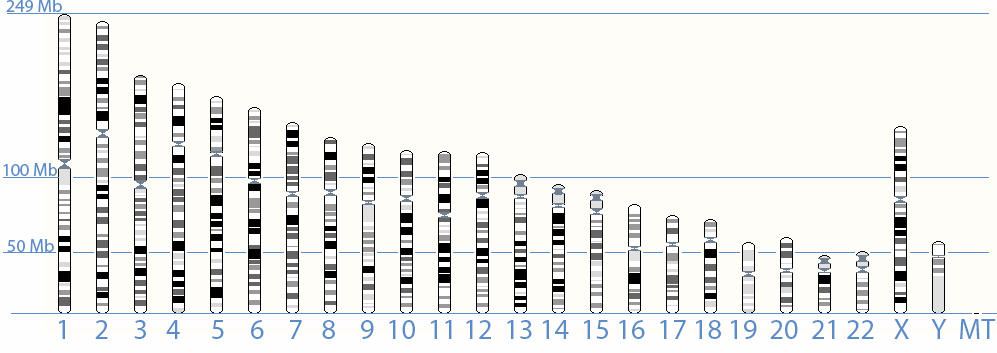
\includegraphics[width=\textwidth]{chromosomes.png}
\caption[Chromosome size comparison]{Chromosome size comparison. Although mtDNA is only $\sim$ 17 kb, due to its high copy number per cell it amounts to approximately 0.1\% to 1\% of the total DNA.}
\label{fig:figureChromosomes}
\end{center}

\end{figure}

\section{Data generation}
\label{sec:dataGeneration}
To attain the informations in the mitochondria respectively their DNA, generally two different approaches exist, being the same as for the nuclear DNA (short nDNA). One approach is to read the whole sequence or a smaller part of it, the other is to look at very specific positions, so called single nucleotide polymorphisms (SNP) of an already known sequence. The technical terms for the two approaches are sequencing and genotyping and are drafted in the following subsections.
\subsection{Sequencing}
Due to the special properties of the mtDNA sequences, often only the non-coding displacement loop (D-Loop) or control region (CR) with about 1 kilobases (kb) is sequenced. This is especially the case in forensics, where it is even more restrictive to the hyper-variable regions 1 and 2 (HVI + HVII) depending on the law policy in the different countries. In clinical studies in most cases the complete 16.6 Kb sequence is  analyzed, since 93.2\% of the nucleotides are in the coding region, responsible for the encoding of the 13 genes to proteins, 22 genes to tRNAs and 2 genes to rRNAs\cite{Sosa2012}. The method used for reading out the mtDNA nucleotides string, is the same as for nucleotide DNA. It has been established by Nobel Laureate Frederick Sanger and colleagues, and is therefore referred to as Sanger Sequencing. The principle idea of this method is essentially the same as happens in nature by replicating the DNA by the enzyme DNA polymerase.
The exception is that an additional `dummy' nucleotide - dideoxynucleotide triphosphate - gets incorporated in the growing DNA chain, causing the reaction to terminate. This reaction can be seen by gel electrophoresis and the incorporated base can be determined. So each incorporation of these dideoxynucleotides (dideoxy ATP or ddATP, ddCTP, ddGTP and ddTTP) terminates at different positions yielding to the final sequence on the autoradiogram.
This method was improved over the years, by using robots running the sequencing reactions and lasers to scan the gel and finally computers to interpret the generated data \cite{WallaceRobertA.SandersGeraldP.1996}. As result we get the whole or partial sequence in a text file, the so called FASTA format after the electropherograms are checked by two different scientists or lab members\cite{Weissensteiner2010}. See figure \ref{fig:figureElectro} for an example of how this data is represented. 
\begin{figure}[ht]
\begin{center}
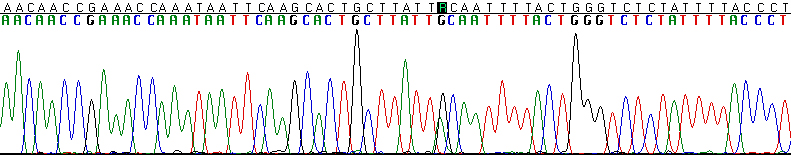
\includegraphics[scale=0.46]{electro9702.png}
\caption[Representation of an electropherogram]{Partial representation of an electropherogram in the Software Sequencher, showing an heteroplasmy on the overlapping curves denoted by R.}
\label{fig:figureElectro}
\end{center}
\end{figure}

A FASTA file begins with the first line containing the symbol \verb|">"| followed by the identifier with no space in between. In the next lines, the nucleotide sequence is provided, where each nucleotide is represented with the initial one-letter abbreviation (nucleic acid code) for \verb|A|denine, \verb|G|uanine, \verb|C|ytosine and \verb|T|hymine. See listing  \ref{lst:fasta} for an example mtDNA sequence file\footnote{the authors mtdna sequence \url{http://www.ncbi.nlm.nih.gov/nuccore/301505865}}. Some special characters exist, like \verb|N| for aNy, \verb|Y| for pYrimidines or \verb|R| for puRine, besides others. In the mitochondrial context, this way heteroplasmies can be described. A FASTA file can also contain alignment characters represented by \verb|"-"|,  or contain amino acid sequences as for protein or peptide sequences with their own amino acid code. Table \ref{tbl:aac} lists the 20 amino acids translated by the corresponding triplets of nucleotides, called codons.

{\small 
\begin{lstlisting}[caption= {Excerpt of an mtDNA fasta file, here the first 350 bases of 16,570}, label={lst:fasta}]
>gi|301505865|gb|HM625680.1| Homo sapiens isolate Lab003 mitochondrion
GATCACAGGTCTATCACCCTATTAACCACTCACGGGAGCTCTCCATGCATTTGGTATTTTCGTCTGGGGG
GTATGCACGCGATAGCATTGCGAGACGCTGGAGCCGGAGCACCCTATGTCGCAGTATCTGTCTTTGATTC
CTGCCTCATCCTATTATTTATCGCACCTACGTTCAATATTACAGGCGAACATACTTACTAAAGTGTATTA
ATTAATTAATGCTTGTAGGACATAATAATAACAATTGAATGTCTGCACAGCCGCTTTCCACACAGACATC
ATAACAAAAAATTTCCACCAAACCCCCCCTCCCCCCGCTTCTGGCCACAGCACTTAAACACA...
\end{lstlisting}
}
\begin{table}[ht]
\begin{tabular}{lccl}
\textbf{Amino Acid}&\textbf{3-Letter}&\textbf{1-Letter}&\textbf{Codon}\\ 
\hline
Alanine&Ala&A&GCA GCC GCG GCT \\ 
Arginine&Arg&R&CGA CGC CGG CGT \\ 
Asparagine&Asn&N&AAC AAT\\ 
Aspartic acid&Asp&D&GAC GAT \\ 
Cysteine&Cys&C&TGC TGT \\ 
Glutamine&Gln&Q&CAA CAG \\ 
Glutamic acid&Glu&E&GAA GAG \\ 
Glycine&Gly&G&GGA GGC GGG GGT \\ 
Histidine&His&H&CAC CAT \\ 
Isoleucine&Ile&I&\underline{ATC} \underline{ATT} \\ 
Leucine&Leu&L&CTA CTC CTG CTT TTA TTG\\ 
Lysine&Lys&K&AAA AAG \\ 
Methionine&Met&M&\textbf{\underline{ATA}} \underline{ATG}\\ 
Phenylalanine&Phe&F&TTC TTT \\ 
Proline&Pro&P&CCA CCC CCG CCT \\ 
Serine&Ser&S&AGC AGT TCA TCC TCG TCT\\ 
Threonine&Thr&T&ACA ACC ACG ACT \\ 
Tryptophan&Trp&W&\textbf{TGA} TGG \\ 
Tyrosine&Tyr&Y&TAC TAT \\ 
Valine&Val&V&GTA GTC \underline{GTG} GTT  \\ 
Terminating codon&&&\textbf{AGA} \textbf{AGG} TAA TAG \\ 
\end{tabular}
\caption[Vertrebrate mtDNA genetic code]{Vertrebrate mtDNA genetic code: 20 Amino Acids translated from the codons. Codons in bold differ from the "Universal" code, underlined codons represent Start-codons. }
\label{tbl:aac}
\end{table}
As represented in the table \ref{tbl:aac}, each of the 13 protein coding genes in the mtDNA \cite{Bandelt2006}, start with either Isoleucine, Methionine or the Valine triplet GTG and are terminated by the triplets in the last row. The listing \ref{lst:fastaAAC} shows the amino acid sequence of the ATP-6 gene\footnote{\url{http://www.ncbi.nlm.nih.gov/protein/ADK77199}}, which starts on position 8527 according to the rCRS so that the first triplet is ATG corresponding to Methionine, represented by M in the protein sequence.
{\small 
\begin{lstlisting}[caption= {Example of a FASTA protein sequence - here the complete ATP-6 gene}, label={lst:fastaAAC}]
>gi|301505871|gb|ADK77199.1| ATP synthase F0 subunit 6 (mitochondrion)
MNENLFASFIAPTILGLPAAVLIILFPPLLIPTSKYLINNRLITTQQWLIKLTSKQMMTMHNTKGRTWSL
MLVSLIIFIATTNLLGLLPHSFTPTTQLSMNLAMAIPLWAGAVIMGFRSKIKNALAHFLPQGTPTPLIPM
LVIIETISLLIQPMALAVRLTANITAGHLLMHLIGSATLAMSTINLPSTLIIFTILILLTILEIAVALIQ
AYVFTLLVSLYLHDNT
\end{lstlisting}
}
The sequence data of published mtDNA is mainly stored in Genbank\footnote{\url{http://www.ncbi.nlm.nih.gov/genbank/}} \cite{Benson2005}, the NIH genetic sequence database. The search term in listing \ref{lst:genbankquery} , yields currently\footnote{as of October 2016} 32,248 homo sapiens sequences, including 12 homo sapiens neandertalensis and 4 homo sapiens subspecies Denisova. 
The correctness of this data is not always given, and has to be handled with precaution. Quality control mechanisms are therefore needed and solutions are presented in chapter \ref{chapterHaplogrep}. 
\begin{lstlisting}[caption={GenBank queries for mtDNA sequences}, label={lst:genbankquery}]
//Homo sapiens
(("Homo sapiens"[Organism] OR Homo sapiens[All Fields]) AND mitochondrion[All Fields] AND complete[All Fields] AND genome[All Fields]) AND "Homo sapiens"[porgn]
//Homo sapiens neanderthalensis
(("Homo sapiens"[Organism] OR Homo sapiens[All Fields]) AND mitochondrion[All Fields] AND complete[All Fields] AND genome[All Fields]) AND "Homo sapiens neanderthalensis"[porgn] 
//Homo sapiens Denisova
Homo sapiens ssp. Denisova 
\end{lstlisting}
\subsection{Genotyping}
In contrast to the previously described method of mtDNA sequencing, genotyping is the process of determining a specific position on a known DNA sequence. Positions of interest are so called single nucleotide polymorphisms (SNPs) as the most common form of genetic variations between individuals \cite{Perkel2008,Brandstatter2003}. The concept of genotyping is to use the known region prior and behind the SNP as so called primers, that bind on the DNA. SNPs were estimated to occur at 1 out of every 1,000 bases on the nuclear DNA \cite{Syvanen2001} in 2001. While in 2008 over 12.8 million SNPs were present in the free public archive Single Nucleotide Polymorphism Database (dbSNP)\footnote{\url{https://www.ncbi.nlm.nih.gov/books/NBK44423/}}, there are about 88 million SNPs present in the 1000 Genome Phase 3 data \cite{Auton2015}, based on 2,504 samples. The work thereby represents DNA composition in 26 populations around the world. 39 million SNPs can be found in European populations, as investigated by the Human Reference Consortium \cite{McCarthy2016} in 2016, based on 30,000 samples. There are about 1,680 SNPs (mtSNPs) on the mitochondrial genome, to be found through Ensembls \cite{Flicek2014} Biomart\footnote{\url{http://www.ensembl.org/biomart/martview/} release Ensembl Variation 86 (GRCh38.p7)}. In over 38 million SNPs provided by the 1000 Genomes Project Consortium Phase 1 \cite{Abecasis2012} 2,834 mitochondrial SNPs (mtSNPs) can be found on the FTP Server\footnote{\url{ftp://ftp.1000genomes.ebi.ac.uk/vol1/ftp/phase1/analysis_results/integrated_call_sets/}}. Figure \ref{fig:figureSNPlocation} represents the SNPs over the mitochondrial genome. When further looking at the rare mtSNPs used for the mitochondrial phylogeny in Phylotree \cite{VanOven2009},\cite{VanOven2010} in the current release 17 based on 24,275 sequences $\sim$ 4,560 different variants or 3,740 transitions, 399 transversions, 50 inserts, 50 deletions and 123 back mutations defining and 5,435 haplogroups) exist. Some of these genotypes are known to cause severe diseases such as Leber hereditary optic neuropathy \cite{Taylor2005} (LHON\footnote{[OMIM 535000] \url{http://omim.org/entry/535000}}) being the most common mtDNA disease leading to blindness. It is caused by one of three mtSNPs 3460A, 11778A, and 14484C in 95\% of all cases \cite{Elson2007}. With technical improvements, the calling of genotypes is performed on platforms like the Sequenom Platform, allowing to genotype 40 SNPs in a sample set of 396 in one run\cite{Weissensteiner2013}, or on a MicroArray per sample, allowing to detect up to 5 million SNPs  \footnote{\url{http://www.illumina.com/Documents/products/datasheets/datasheet_gwas_roadmap.pdf}}, where up to 4,000 mitochondrial variants\footnote{\url{https://www.livingdna.com/en-gb/help-centre/87/what-technology-behind-procedure}} are included.

\begin{figure}[ht]
\begin{center}
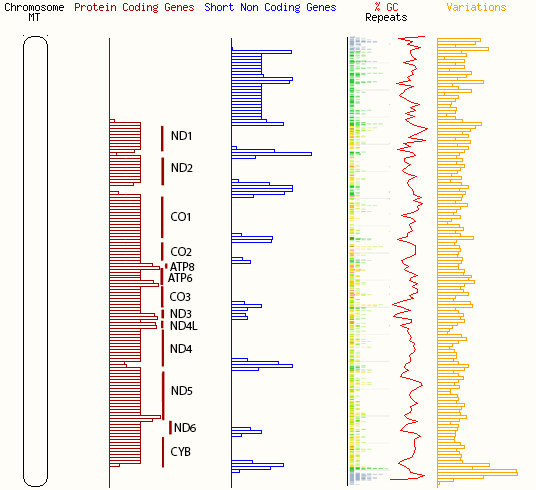
\includegraphics[scale=0.7]{ensembl_mt2.png}
\caption[mtSNPs location on mtDNA]{Overview of the mtSNPs and their location on the mtDNA. Figure modified from UCSC Genome Browser\footnote{\url{https://genome-euro.ucsc.edu/index.html}}}
\label{fig:figureSNPlocation}
\end{center}
\end{figure}

\subsection{Next Generation Sequencing (NGS)}
The step from conventional Sanger Sequencing to NGS revolutionized the genomics research area, however it came also with two shortcomings for the latter: read length was very short (about 36 base pairs\cite{Li2013a} in the beginning compared to 1,000 base pairs in Sanger) and the error rate a tenfold higher. New algorithms were required for assembling the short reads to a reference genome (called mapping) if already available or to a de novo sequence, in the case no reference sequence can be used. The big advantage of NGS over Sanger Sequencing is the amount of data throughput (several hundred Gigabases per Run instead of some Kilobases), the speed and the much lower cost per base. Hundreds of mtDNA samples can be processed in one run, by generating high-coverage mtDNA sequences. 
The classical FASTA format was extended to so called FASTQ files, where besides the nucleotide sequence also their quality scores are stored as ASCII characters (see Data description \ref{datadescription}). Additional files for storing the mapping as well as for the called variants are now de facto standards, and are presented within this subsection. 
\section{Data description}\label{datadescription}
With almost every sequencing-device vendor having its own file format, the first step after a successful run, is the conversion of the primary analysis results in form of images of some terabytes to its own FASTA like sequencing file. There are different FASTQ file encoding (Sanger, Solexa, Illumina), Color Space Fasta files (.csfasta for ABI SOLiD) or Standard Flowgram Files (SFF for Roche and Ion Torrent). The raw FASTQ files are mapped to a reference sequence in order to compare the results and based on this mapping, the variant calling can be performed, yielding to VCF files. The next subsections represent the data and how it is structured. 
\subsection{Raw Reads: FASTQ file}
For the described application in Chapter \ref{chap:NGS}, the  direct support of FASTQ files of different encodings is required. SFF (by Roche) and color space (csfasta, by Thermo Fisher Scientific) files, besides others\footnote{\url{https://www.ncbi.nlm.nih.gov/sra/docs/submitformats/}} can be converted straight forward to FASTQ, which nowadays is the standard format for NGS results.  
Listing \ref{lst:fastq} shows the structure of a FASTQ file. 4 rows characterize one read. This has to be taken into consideration, as shown in Chapter \ref{chap:NGS}, when splitting up files at fixed sizes as it is the case in MapReduce with its 64 MB blocks. Listing \ref{lst:fastq} depicts the structure, where the first row indicates the read-number, the second row represents the actual nucleotide sequence, the third row is optional and mostly consisting of the symbol {+} only and the fourth row represents the base quality, encoded in ASCII code. So the first nucleobase G with ! as ASCII character has numerical value of 33 being the first printable code, the base A has value 39 (') see  ASCII Codes Table\footnote{\url{http://ascii.cl/}}. Read length varies usually between dozens to some hundred bases (e.g. for Ion Torrent depending on chemistry up to 400 base pairs) or can be a fixed length (101 nucleotides for the Illumina HiSeq). Depending on the device data can be so called single- or paired end. In contrast to single-end, paired-end sequencing is characterized by 2 resulting FASTQ files per sample, where reads from both files are checked based on their read number and provide a much higher accuracy and are more likely to map to a reference\footnote{\url{http://technology.illumina.com/technology/next-generation-sequencing/paired-end-sequencing_assay.html}} since the reads come from the same fragment from both ends.
\begin{lstlisting}[caption= {Excerpt of an FASTQ file, 4 rows representing one read}, label={lst:fastq}]
@SEQ_ID
GATTTGGGGTTCAAAGCAGTATCGATCAAATAGTAAATCCATTTGTTCAACTCACAGTTT
+
!''*((((***+))%%%++)(%%%%).1***-+*''))**55CCF>>>>>>CCCCCCC65
\end{lstlisting}
\subsection{Aligned reads: BAM file}
Besides the previously presented "`raw"' sequence format, some defacto standards in the NGS environment are presented in this paragraph. The most established being the Sequence Alignment/Map (SAM) format \cite{Li2009} supporting single- and paired-end reads. It can include different raw formats (not only FASTQ) such as the before mentioned color space reads. The format consists of 2 sections for header and alignment informations. Header content is characterized by "`@"' symbol, the alignment informations are tab delimited and require 11 mandatory fields. Listing \ref{lst:sam} shows an example SAM file\footnote{\url{http://samtools.github.io/hts-specs/SAMv1.pdf}} 
\begin{lstlisting}[caption= {Excerpt of a SAM file, representing two reads}, label={lst:sam}]
@HD VN:1.5 SO:coordinate
@SQ SN:ref LN:45
r001 99 ref 7 30 8M2I4M1D3M = 37 39 TTAGATAAAGGATACTG *
r002 83 ref 9 30 3S6M1P1I4M *  0  0 AAAAGATAAGGATA    *
\end{lstlisting}
The CIGAR string in column 6 (for r001: 8M2I4M1D3M) represents the read and it's operations needed to be mapped to a reference string. The operations are M for Match, I for Insertion, D for Deletion and S for Substitution. 
The quality scores are the same as in the FASTQ file, given as Phred-scaled quality values where $\left( Q=-10\log_{10} P\right)$ where $P$ is the probability that the base call is correct\cite{Loman2012}. Additionally tags in the form of key value pairs can be provided in the last column, however in the example not used (denoted by the symbol *).
A BAM file is the binary representation of a SAM file, hence much smaller in file size. Both SAM and BAM files have an Index (called .sai or .bai respectively), and are sorted, so that direct access to a region of interest is guaranteed and not the whole file has to be processed. This is of special interest when downloading of a small region like the mitochondrial genome covered in a Whole Genome Sequencing run should be carried out. Instead of downloading about 120 GB (for a high-coverage whole-genome experiment with coverage ~40x) per sample, only approx. 100MB are downloaded (depending on the mitochondrial copy number present in the sample).
\subsection{Variants: VCF file}\label{intro:VCF}
To get the specific mutations from a BAM file, a variant calling step is required. There are many tools available to perform this step, and provide a VCF file, where the results per sample and per position on the DNA are listed. The structure of the VCF files is maintained by the Global Alliance Data Working Group File Formats Task Team \footnote{\url{http://ga4gh.org/\#/fileformats-team}}. The specifications can be found on the GitHub page\footnote{\url{https://vcftools.github.io/specs.html}}. Summed up, it is a text file that has meta-information lines about genotype informations before the actual header line which can contain different columns, requiring 8 fixed fields, as represented in Table \ref{table:vcf}. After these fixed columns, Sample Ids can be appended, separated by tab, containing the genotype information ("`GT"') per position, or extended to customized informations such as nucleobases and base count for next-generation sequencing data.

\begin{table}[H]
  \begin{tabular}{lll}
    \toprule
    Field & Description & Example \\
		\midrule
    \#CHROM & Number of Chromosome & MT or chrM \\
    POS & Position of the variant/SNP & 73, 263,.. \\
    ID & ID of the SNP, otherwise "`."' & rs3087742, .\\
    REF & base on reference & A, A, ...\\
    ALT & transition/transversion & G, G,C...\\
    QUAL & quality as phred score & 50 \\
    FILTER & all filters passed & PASS \\
    INFO & additional information & CIGAR \\
		\bottomrule
\end{tabular}
\caption{Fixed fields in an VCF file, the new standard format for called variants}
\label{table:vcf}
\end{table}

\section{Conclusion}
In this chapter the biological foundations and definitions of data formats used within the next chapters of this work, were presented. Mitochondrial DNA was introduced, by comparing it to the nuclear DNA. It has the property to be inherited only maternally in humans, which renders it an ideal tool for studying the evolution of homo sapiens, as well as different species, back to the most recent common ancestor. This allows the creation of phylogenetic trees, presented in the next chapter. Thereby the data can be produced with different methods and devices. The mtDNA can be analyzed on single positions called SNPs or read out as complete sequence. Depending on the method, various file formats are produced (i.e. FASTA or FASTQ files). Processing the raw input data introduces new file formats especially for the next-generation sequencing with BAM or CRAM files and VCF files for the called variants. Tools for processing these mtDNA data are presented in the subsequent chapters.
\cleardoublepage
\chapter{HaploGrep: an Algorithm for mtDNA Classification to Haplogroups}
\label{chapterHaplogrep}
Human mitochondrial DNA being a non-recombinant DNA, is strictly inherited maternally. Mutations which occur over the time and get fixed mutations by passing on to the next generation, undergo a so called positive selection. Negative selection imposes the ending of a germline. So, in theory, if no mutations would occur on the mitochondrial genome, all eukaryotes from the first "mitochondrial Eve" or often also referred to as \textit{Most Recent Common Ancestor} (MRCA) to the current living human beings, all should carry the same mtDNA sequences. However over the time, mutations accumulated (and still do), which are passed on to the following generations \cite{Stewart2014}, rendering it possible to reconstruct a tree of life. This is not only affecting humans, but all eukaryotic beings (including the 4 kingdoms Plantae (plants), Fungi, Protista (unicellular organisms) and Animalia including homo sapiens). The mutation rate of the human mtDNA is much higher than the one for the nuclear DNA. The substitution rate is about 1.665 x $10^{-8}$ ($\pm$ 1.479 x $10^{-9}$) per base per year or one mutation every 3,624 years to get a fixed mutation on the mtDNA \cite{Soares2009}. This makes mtDNA an ideal tool for reconstructing the human ancestry by confirming the out of Africa theory and helping to understand the colonization of humans over the time on the various continents. The branches of this phylogeny or tree are called haplogroups, comprising a collection of related individuals with their mutually shared mitochondrial haplotypes \cite{Scally2012}. \\
Knowing the mtDNA haplogroup affiliation is a critical prerequisite \cite{Kloss-Brandstatter2011} for studying mechanisms of human evolution and discovering genes involved in complex diseases. Besides these applications, validating phylogenetic consistency using haplogroup classification gains importance in quality control. 

Despite the availability of \textit{Phylotree} \cite{VanOven2009}, a regularly updated classification tree of global mtDNA variation, the process of haplogroup classification was time-consuming and error-prone \cite{Kloss-Brandstatter2011}. Thereby researchers have to manually compare the polymorphisms found in a population sample to those summarized in Phylotree, polymorphism by polymorphism, sample by sample. To circumvent these limitations, this chapter provides a solution to the problem of haplogroup classification based on given mitochondrial DNA profiles. The application called HaploGrep presents a fast, reliable and straight-forward algorithm and is implemented as a freely accessible web application. The presented method is able to determine the haplogroup affiliation of thousands of mtDNA profiles within seconds \cite{Kloss-Brandstatter2011}, otherwise cumbersome compiled by hand. The input profiles can represent the whole mitochondrial genome, or any part of it from sequencing projects, as well as just specific genotypes information as derived with of microarrays or genotyping platforms. HaploGrep is based on the latest version of Phylotree (currently mtDNA tree Build 17 (18 Feb 2016)) by offering scientists in various areas (i.e. clinical genetics, population genetics, archeoegenetics or forensics) an all-in-one solution for quality assessment of mtDNA profiles, with high accurate haplogroup results. \\
This chapter starts with an overview on the different tools currently available for the haplogroup classification of mitochondrial genomes (see Section \ref{hg:related}), provides insights in the methods and algorithms implemented in the presented solution HaploGrep (see Section \ref{hg:haplogrep}) by comparing its performance with tools from the related work section. Further different alternative algorithms are presented and the dissimilarity distances (see Section \ref{hg:dissimilarity}) are also compared regarding run-time and accuracy. An important aspect of the analysis of mitochondrial genomes with the phylogenetic information provided by Phylotree on hand, is the feature of quality control (see Section \ref{hg:qc}). For instance, if a sample shows mutations belonging to two different haplogroups, this could indicate artificial recombination in the lab. There are several other possible sources of issues, sample swap or contamination, that can be located based on phylogenetic trees. This chapter ends with a conclusion \ref{hg:outlook} and gives an outlook on the features for a future update.  
\section{Related Work}\label{hg:related}
When we first described our haplogroup classification approach in 2010 \cite{Kloss-Brandstatter2011}, only few automatic approaches for haplogroup classification where present. By then we ware aware two tools both showing some weaknesses, that were presented in our paper: mtDNAmanager \cite{Lee2008}  and MitoVariome \cite{Lee2009}. Since there was an obvious demand for such tools, several new approaches were published thereafter. Table \ref{table:tools} gives an overview of the automated mtDNA haplogrouping methods available as of October 2016. As can be seen, there's still a huge interest of the mtDNA community to improve the haplogrouping tools. 

\begin{table}
  \begin{tabular}{lllll}
    \toprule
    Method  & Year &  Reference & Cited $^*$\\ 
		\midrule
		mtDNAmanager & 2008 & Lee et al. \cite{Lee2008} & 66\\ 
		MitoVariome & 2009  & Lee et al. \cite{Lee2009} & 12\\
		mtPhyl & 2009 &  Eltsov and Volodko \cite{eltsov2009mtphyl} & \#\\
		Ensemble Learning & 2010 &  Wong et al. \cite{Wong2011} & 11  \\ 
		\textbf{HaploGrep} & \textbf{2010} & \textbf{Kloss-Brandst{\"a}tter et al.} \cite{Kloss-Brandstatter2011} & \textbf{261}  \\ 
		mthap & 2010 & Lick& \# \\ 
		MitoTool & 2011 & Fan and Yao \cite{Fan2011} & 78\\
		HaploSearch & 2011 & Fregel et al. \cite{Fregel2011}  & 15 \\
		HmtDB: mt-classifier & 2012 & Rubino et al., \cite{Rubino2012}& 64 \\
		mtdnacommunity & 2012 & Behar et al. \cite{Behar2012} (RSRS) & 245\\
		mtDNAoffice & 2012 & Soares et al. \cite{Soares2012} & 3 \\
		EMMA & 2013 & Roeck et al. \cite{Rock2013} & 42\\
		Updated MitoTool& 2013& Fan and Yao \cite{Fan2013} & 40\\
		HaploFind & 2013 & Vianello et al. \cite{Vianello2013} & 39\\
		Phy-Mer & 2014 & Navarro-Gomez et al. \cite{Navarro-gomez2014} & 11\\
		\textbf{HaploGrep 2} & \textbf{2016} & \textbf{Weissensteiner et al.} \cite{Weissensteiner2016a}  & \textbf{21}\\
        HmtDB 2016  & 2017 & Clima et al. \cite{Clima2017}&  \\

		\bottomrule
\end{tabular}
\caption[Related work]{Overview of automated haplogrouping tools for human mtDNA, $^*$number of citations as of June, 2017 in Google Scholar (\url{https://scholar.google.com/}) \# tool not published in a peer reviewed journal} 
\label{table:tools}
\end{table}

Thereby different methods for the haplogroup classifications are applied by the various approaches. \textbf{mtDNAmanager} used algorithms based on propositional logic via hierarchical verification, without further specifying the algorithm in detail. On a predetermined list of control region mutation motifs which are stored in a MySQL database, a query system accepts the classification requests and returns the most-probable mtDNA haplogroup based on 9,294 control region sequences. The match probability is estimated by the frequency of a haplotype by $(x+2)/(n+2)$ according to Balding and Nichols \cite{Balding1994}, where $x$ is the number of times a haplotype appears in the database of size $n$. A limitation is however the use of the mtDNA control region only (16024–16569; 1–576), being often to coarse for an exact haplogroup classification.\\
\\
\textbf{Mitovariome} by Lee et al. \cite{Lee2009} is another database of precalculated sequences, allowing to query for polymorphism, haplogroups and GenBank accession numbers. However, it wasn't maintained further and is not available any further.\\
\\
\textbf{mtPhyl}\label{mtphyl} which was not published in a journal, but only presented at the ASHG meeting in 2008 presents one of the most unknown but most influencing tool in the field of haplogrouping. It applies a maximum parsimony-based method for reconstructing the mtDNA phylogeny, estimates the mitochondrial haplotype and calculates the coalescence time of clusters. Based on the phylogenetic reconstruction by this tool, the current human mitochondrial phylogeny represented by Phylotree was enabled which is still subject to a continuous update process \cite{VanOven2015}. mtPhyl can be downloaded from \url{https://sites.google.com/site/mtphyl/home}\\ 
\\
A completely different approach for haplogroup estimation was presented by Wong et al. \cite{Wong2011}. By the use of two different \textbf{machine learning approaches}, the limitations of earlier used nearest-neighbor methods were tried to solve. Based on Principal Component Analysis (PCA) and the\textbf{ Random Forest} (RF) algorithm (being an ensemble learning algorithm) haplogrouping was performed. The second method presented was a \textbf{Support Vector Machine} (SVM) algorithm. Both methods are requiring training data sets. The overall macro-accuracy of the two methods were 87.35\% and 88.06\% respectively, indicating problems with some particular haplogroups (especially haplogroup R* and N*, with a macro-accuracy of $\sim$ 10\% and 49.21\% for RF and 11.67\% and 52.38\% respectively). \\
\\
\textbf{mthap} was developed since 2010 on private initiative of James Lick and addresses data input for single samples. It is not intended for academic purpose but helps individuals interpreting their data from direct-to-consumer personal genome tests (for example 23andMe\footnote{\url{https://www.23andme.com/}} data).\\
\\
\textbf{MitoTool} was published in 2011 and got updated in 2013. It comes with an own database with currently 22,525 mtDNA sequences according to Phylotree 15 and allows detailed parsing and annotation of FASTA and variants input data. It is suitable for both, rCRS and RSRS references, and allows the transformation of a FASTA-like format to each other. The updated version comes with a stand-alone version, which is often required for complying with data privacy laws, especially in the field of forensics and clinical research. The similarity parameter $S$ is calculated for each haplogroup where $S=2M-N$ for $M$ representing the number of shared variants between query and tested haplogroup and $N$ being the number of all variants required by the currently tested haplogroup. The complexity is thereby $O(n)$ where $n$ represents the amount of comparisons of haplogroups present in Phylotree.\\
\\ 
\textbf{HaploSearch} was designed to get the variants from a multiple-alignment format FASTA file or to generate multiple-alignment FASTA sequences from variants. This way it is more flexible and can be used also for non-mtDNA data. HaploSearch determines the haplotype, but no classification to haplogroups is provided. The project web-site is not available any further (last accessed May 2017).\\
\\
The human mitochondrial genomic resource HmtDB provided its haplogroup prediction tool \textbf{fragment-haplo-classifier} in 2012 which later was updated to the \textbf{mt-classifier} tool as part of the MToolBox pipeline and the HmtDB update 2016. It is Python based and relies on the RSRS reference. It allows the classification of haplogroups based on Phylotree, by accepting FASTA files which are aligned by using Muscle. The distance measurement is similar to MitoTool, where variants from the query sequence are mapped to haplogroups predefined in Phylotree (referred to as $N_{ph}$) are set in relation to the expected number over the the corresponding region (denoted as $Nph_{exp}$), resulting to the prediction percentage per haplogroup $P_{Hg}=N_{ph}/Nph_{exp}$, where only values $>90\%$ are emitted as results.\\
\\
In 2012 the discussion about the human mitochondrial genome reference sequence got a new attention. Behar et al. introduced the Reconstructed Sapiens Reference Sequence (RSRS) as a "Copernican" reassessment of the human mtDNA phylogeny \cite{Behar2012}. While there are good reasons to this change-over, it can lead to additional confusion especially in the forensics and clinical research \cite{Bandelt2013}. The presented online appearance mtDNAcommunity.org\footnote{\url{http://www.mtdnacommunity.org}} provides tools for transformation (FASTmtDNA) as well as haplogroup labeling and phylogeny-based quality control with \textbf{mtDNAble}. The method behind mtDNAble was not described in detail.\\
\\
With \textbf{mtDNAoffice}, Soares et al. \cite{Soares2012}, present a human mtDNA macro haplogroup assignment tool for the protein coding region of the mitochondrial genome. Thereby a vectorial representation method was used, by "naturally aligning mtDNA protein-coding region" \cite{Soares2012}, in a first step. The resulting genetic distance matrix was used to construct neighbor-joining or an Unweighted Pair Group Method with Arithmetic Mean (UPGMA) tree. Excluding the hyper-variable control region as input is however limiting the accuracy of haplogroup estimation.\\
\\
The Institute of Legal Medicine (GMI) at Innsbruck was developing \textbf{EMMA} in 2013 together with Mannis van Oven, author of Phylotree, being also involved in \textit{mtdnacommunity} and \textit{Phy-Mer}. Based on a combination of database and the use of Phylotree, haplogroup estimation is performed by applying a maximum likelihood ranking. Maximum-Likelihood Estimation (MLE) was applied earlier by the Genographic Consortium \cite{Rosset2008} successfully for site-specific mutation rates in mtDNA, where only partial phylogeny was taken into consideration. After estimating the fluctuation rate per variant, the cost function in EMMA was denoted as $C_t(b) = \sum_i{c(b_i,t_i)}$ by $i$ iterating over all positions where the query ($t$) and the currently tested profile ($b$) differ, by scaling the positional costs logarithmically to  $c(b_i,t_i)= lg(r(t_i \rightarrow t_i)/r(b_i \rightarrow t_i))$. \\
\\
\textbf{HaploFind} performs the haplogrouping according to the RSRS as reference sequence for complete sequences. It makes use of the suffix-tree based algorithm Mummer for sequence alignment and comparison which is performing great, but needs careful handling of variants, since the nomenclature can differ to phylogenetic standards. The algorithm for haplogroup classification is based on the pre-calculated variant scores from $\sim$ 7,800 samples. The assignment is processed in a recursive manner, where query and the tested haplogroup "are compared by searching for matches, summing to the sequence score the score of each matching variant" \cite{Vianello2013}.\\
\\
\textbf{Phy-Mer} is an approach from 2014, to perform haplogroup classification directly on sequencing data, without an actual alignment by further being reference independent. It is one of the first mitochondrial haplogroup classification tools to take data from NGS devices in form of FASTQ or BAM files into account. Using a k-mer library based on sequences from Phylotree, the distances to the query sequence are calculated by comparing the sets of all possible k-mers. \\

\section{HaploGrep}\label{hg:haplogrep}
This Section describes our approach to automatically classify mtDNA profiles into haplogroups as one of the first tools being directly based on the data from Phylotree.
\subsection{Architecture}
HaploGrep was initially implemented as a Java application with several modules, and got extended to a Web application on a client-server architecture. The first module is the parser based on JExcelApi\footnote{\url{http://jexcelapi.sourceforge.net/}} for spreadsheet input files. Phylotree provides the clearly structured data as HTML versions for manual navigation from an Microsoft Excel sheet. We therefore re-coded the XLS file to a XML file by using the standard libraries provided by Java. For every new update of the Phylotree versions to be used with HaploGrep, three steps are required: 
\begin{enumerate}
\item In a first preprocessing step directly incorporated in Excel (written in Visual Basics for Application (VBA)), the data integrity of the XLS file is checked (i.e. missing lines or empty labels). 
\item Thereafter the actual transformation from XLS to XML is generated with our parser. It runs recursively over the XLS file and writes the haplogroup name, all profiles, accession number and references if provided hierarchically to the XML file. HaploGrep relies on the rCRS, hence all profiles are reported as list of nucleotide positions that deviate from this reference. 
\item The newly generated XML file is parsed for generating the fluctuation rates per position. The corresponding algorithms used can be found in the next subsection \ref{hg:algorithm}.
\end{enumerate}
As mentioned, the core of HaploGrep is implemented as a Java library, with a web client. This way all the computational intensive tasks are performed on server side, by getting use of REST for the client-server communication, implemented within the Restlet Framework. For every request a server side generated session object is created and encrypted through a session key. The XML based tree is loaded once in an in-memory hash table, increasing HaploGrep's speed significantly compared to other methods (see Figure 3 in \cite{Kloss-Brandstatter2011}). We also take advantage of current multi-core architectures by handling requests efficiently in concurrent ways. We take advantage of multi-threading by using Java's \verb|java.util.concurrent| packages, by using mostly \verb|ConcurrentHashMap| and \textit{worker threads} by using \textit{thread pools}, which reduce overhead due to thread creation, avoiding memory management overhead otherwise caused by allocating and deallocating many thread objects\footnote{\url{https://docs.oracle.com/javase/tutorial/essential/concurrency/pools.html}}. \\
The front-end of the client is implemented in JavaScript as HTML5-based Rich Internet Application, by using the EXT-JS JavaScript MVC framework\footnote{\url{http://www.extjs.com}}. The communication is AJAX based, which means we use asynchronous HTTP requests, with the earlier mentioned REST-resource, by using JSON\footnote{\url{http://www.json.org}} and XML as standard exchange formats. For the graphical representation of the Phylotree, the InfoVis Toolkit \footnote{\url{http://thejit.org}} is applied. Additionally BioJava \cite{Prlic2012} and the high performance collections library Trove\footnote{\url{http://trove.starlight-systems.com/}} where used for the input of FASTA sequences, which outperform JDK's collections by applying open addressing for primitive types (see Chapter \ref{chapterAlignment}). The HTSJDK Java API provided by the Broad Institute\footnote{\url{https://github.com/samtools/htsjdk}} was integrated for the import of VCF (Variant Call Format) files.

\subsection{Input Data Formats}\label{hg:input}
Besides the own data input format defined in the first version of HaploGrep called \verb|*.hsd| format, HaploGrep 2 supports several new data input formats. 
The *.hsd file is a simple tab delimited text file, which consists of at least 4 columns; ID for the sample identifier, the targeted mtDNA region, either as range separated by "-" or single SNPs separated by ";", the haplogroup if already estimated, and the polymorphisms separated by tabs. Table \ref{table:hsd} gives an example of HaploGrep's standard input format.
The format is similar to the EMPOP format \cite{Parson2007}, with the main difference that the range can be specified directly per row.
\begin{table}[H]
  \begin{tabular}{lllllll}
    \toprule
    ID & Range & Haplogroup & SNP &  &  \\
		\midrule
	Sample1 & 16024-16569; &  & 16051G & 16051G & 16182C\\
	Sample2 & 16024-16569;1-576; &  & 16224C & 16311C & 146C\\
	... & ... & & ... & & & \\
		\bottomrule
\end{tabular}
\caption{Example of an *.hsd file, the standard input format for HaploGrep}
\label{table:hsd}
\end{table}

HaploGrep in the updated version 2 accepts further input formats, being FASTA files and VCF files. While for the FASTA import there exist different implementations, one requiring an additional alignment step, the use of HTSJDK allows the direct import of VCF files. The files are parsed and converted so that the internal objects can be used, which were designed for the hsd files (see Chapter \ref{chapterAlignment} for the methods behind the alignment step). 
\\
The structure of the VCF files was presented in the Introduction (see Section \ref{intro:VCF}). As short repetition, the file is tab-separated, with 8 fixed fields or columns, that are compulsory, and can be extended to the users need\footnote{\url{https://vcftools.github.io/specs.html}}.

\subsection{Algorithm for Haplogroup Classification}\label{hg:algorithm}
The main idea behind HaploGrep is the usage of Phylotree as database, by calculating for each variant occurring in the tree a so called phylogenetic weight. This weight is an assessment of the stability of a SNP. In the first version of HaploGrep the following method for assigning the phylogenetic weights is used: by traversing the Phylotree, for every mutation the amount of occurrence gets estimated. The SNP with the highest occurrence + 1 (i.e. m.152T$>$C occurred 106 times in Phylotree 10 used for the publication) is taken as reference value. The weight is obtained by subtracting the number of occurrences from the reference value \cite{Kloss-Brandstatter2011}. This way SNPs with higher occurrence get a lower weight than SNPs occurring only once. Hotspot Mutations like m.16519T$>$C were assigned values 0 (see Algorithm \ref{alg:haplo1}).

\begin{algorithm}
\caption{Scoring of weights in the first version of HaploGrep}
\label{alg:haplo1}
The index set $I$ refers to all mutations found at least once in PhyloTree. 

For each $i \in I$ let $f_i$ be the absolute frequency of mutation $i$ on the current build of PhyloTree. 

Let $F$ = $max(i_{fi})$ be the maximum of all those frequencies. 

For $i \in I$ put the weight $w_i = F-f_i$ \cite{Kloss-Brandstatter2011}. 
\end{algorithm}

As an example, consider the demonstration provided in our publication \cite{Kloss-Brandstatter2011}: assume that a sample was sequenced for the entire control region (nucleotide positions 16024–16569; 1–576) and genotyped for 45 coding region SNPs as described by Brandstaetter et al. It showed the following profile (with corresponding weights): m.263A$>$G (105), m.309 - 310insC (0), m.315 - 316insC (0), m.750A$>$G (106), m.951G$>$A (103), m.8860A$>$G (106), m.15326A$>$G (106), m.16354C$>$T (101), and m.16519T$>$C (0). The polymorphisms m.309 - 310insC, m.315 - 316insC, and m.16519T$>$C were hot spots and therefore not taken into consideration (weighted with 0). For every haplogroup the rank was calculated according to HaploGrep's algorithm: haplogroup H2a1 was rated best because all diagnostic polymorphisms for the haplogroup were found in the sample $[(105+106+103+106+106+101)/(105+106+103+106+106+101) = 1]$ and none of the sample’s polymorphisms remained unexplained or private $[(105+106+103+106+106+ 101)/(105+106+103+106+106+101+0+0+0)=1]$. Therefore, the overall rank for H2a1 was $r_{H2a1}=0.5\times 1.0 + 0.5 \times 1.0 = 1.0$. For example, the third best hit was haplogroup H2a, where the value for the first part of equation was still 1.0 but because two polymorphisms (m.951G4A, m.16354C4T) remained unexplained in the sample’s profile, the second part of the equation was $(105+106+106+106)/(105+106+103+106+106+101+0+0+0) = 0.6746$, thus leading to a final rank of $r_{H2a}= 0.5\times 1.0 + 0.5\times 0.6746 =0.837$ \cite{Kloss-Brandstatter2011}. \\
In the updated version of HaploGrep 2, this value was classified with a more sophisticated phylogenetic weight, where we scaled the weights in a window from 1 to 10 (see Algorithm \ref{alg:haplo2}).
\begin{algorithm}
\caption{Scoring of weights in the new version of HaploGrep 2}
\label{alg:haplo2}
Let the index set $I$ refer to all mutations found at least once in PhyloTree $P$.

For each $i \in I$ let $f_i$ be the absolute frequency of mutation $i$ in $P$. 

Let $F$ = $max(i_{fi})$ be the maximum of all those frequencies. 

For $i \in I$ calculate the weight $w_i = 1+(9/\ln(F)) \times [\ln(F) - \ln(f_i)] = 10-9\ln(f_i) / \ln(F)$. 

Conversely, given $1 \leq w \leq 10$, the corresponding frequency $f$ is calculated as  $f = F(10 - w)/9$ \cite{Weissensteiner2016b}.
\end{algorithm}

Based on the calculated weights per variant $w_i$ we calculate for every haplogroup in phylotree the distance to the query variants $r_{hg}$, where we take into account how often variants are found per haplogroup ($k$), the number of variants expected in the analyzed range of the tested haplogroup ($m$) and the total number of polymorphisms in the query sample ($k$).

\begin{equation}
	r_{hg} = \frac{1}{2} \times \left(\frac{\sum^{k}_{i=1} w_i}{\sum^{m}_{i=1} w_i} + \frac{\sum^{k}_{i=1} w_i}{\sum^{n}_{i=1} w_i}\right)
\end{equation}

Thereby the formula shows that this rank is composed of two parts. The first component calculates the weighted ratio of haplogroup-associated polymorphisms that were found in the sample to the total number of haplogroup-associated polymorphisms in the currently tested haplogroup within the analyzed range. The second part reflects the ratio of polymorphisms in the test sample that are associated with the haplogroup under investigation to the total number of polymorphisms found in the test sample \cite{Kloss-Brandstatter2011}. This second component assures that a result will be ranked higher if it uses as many polymorphisms in the sample as possible \cite{Kloss-Brandstatter2011}. The two components are weighted equally and form the final overall rank $r_hg$. The resulting list is sorted according to these ranks to present the user the best results first  \cite{Kloss-Brandstatter2011}. When we first described this algorithm, we weren't aware that this formula was described by Stanisław Kulczyński in 1927. The Kulczyński Similarity Measure 2 is a similarity for numerical data in $\mathbb{R}^n$, according to \cite{Deza2009}:
 
\begin{equation}
\frac{n}{2}\left(\frac{1}{\overline x}+\frac{1}{\overline y}\right) \sum{min(x_i, y_i)}
\end{equation}

where $x$ and $y$ represent non-zero vectors ($x=(x_1,...,x_n)$ and $y=(y_1,...,y_n)$). $\overline x$ denotes $\frac{\sum{x_i}}{n}$ corresponding to the \textit{mean value} of components $x$. Same holds true for $\overline y$. $n$ is the length of the vectors.

Since we parse the Phylotree as a structured XML tree in memory, by loading it once, queries are handled in a recursive manner. Listing \ref{list:pseudo} represents the calculation of the ranks where $max(r_{hg})$ represents the best hit.

\begin{algorithm}
\caption{Querying profiles recursively against the Phylotree database}
\label{list:pseudo}

For node $n_{i}$ in Phylotree $P$ with $i=0; i<|P|$ get all child nodes $n_{i_{firstChild...lastChild}}$

For all polymorphisms $p$ in $n_{i}$ and in range $R$ calculate Arrays in steps 3-7, by considering the query input sample $Q$ polymorphisms $q_{1}..{|Q|}$:

Expected add $p$

Found add $p$ if $p$ $\in$ $Q$ and $p$ $\in$ $R$ 

Remaining add $q$ if $q$  $\in$ $R$ and $\not\in$ $n_{i}$

Notfound add $p$ if $\in$ $R$ and $\not\in$ in $Q$

Out add $p$ $\not\in$ $Q$ and $\not\in$ $R$

calculate rank of haplogroup $(r_{hg})$ based on weights $w$ of polymorphisms in arrays according Algorithm \ref{alg:haplo2}

$Result[r_{n_{i}}]$ = $ \frac{1}{2}\left(\frac{w_{Found}}{w_{Expected}} +  \frac{w_{Found}}{w_{Q}}\right)$

For each child nodes repeat steps 1-9

While parent node not root-node, get parent node of $n_{i}$ and start at 1

result = $\max (Result[r_{n_{i}}]) $

\end{algorithm}



\subsection{Output formats}

The main concept of HaploGrep, is to provide all relevant data immediately in the browser, after the haplogroup classification is performed automatically after the file upload. Also the file-exports are represented in a graphical way in the browser prior the download by the user. Several new browser- and file-based outputs can be generated:
\begin{enumerate}
\item Haplogroups Report: all the data generated for the haplogroup classification are summarized in a table. The information provided comprises the resulting haplogroup per sample, with its quality score (default Kulzczynski-distance). Further the not assigned remaining polymorphisms, the polymorphisms not found in the top ranked haplogroup are listed, as well as the annotation of the corresponding amino acid changes provided in Pereira et al. \cite{Pereira2011} and the input profile.
\item Multiple Alignment Format: based on the rCRS reference sequence, HaploGrep provides a multiple sequence alignment format. This format aligns all sequences to the same length, by extending it for insertions if present. Deletions are denoted with "-" and handled identical to base substitutions. This way a cost intensive multiple sequence alignment is reduced to a pairwise alignment, with an additional help of a vector storing the insertions and deletions. The details can be found in Chapter \ref{chapterAlignment}. The  generated multiple sequence alignment in FASTA format and can be directly viewed in the browser. This is based on the implemented BioJS open source JavaScript framework for biological data visualization \cite{Gomez2013}. Having the multiple alignment format at hand, the freely available tool PGDSpider \cite{Lischer2012} can be used subsequently for downstream analysis. Thereby the multiple-alignment result can be converted into a variety of population genetics formats. Some of the well established tools supported this way are ARLEQUIN \cite{Excoffier2010}, MEGA \cite{Tamura2013}, MIGRATE \cite{Beerli2010}, PHYLIP \cite{Felsenstein1989} directly or the NEXUS format \cite{Maddison1997} for MRBAYES \cite{Huelsenbeck2001} or PAUP* \cite{Swofford2003} as listed in \cite{Weissensteiner2016a}.
\item VCF: a column-based representation of all samples is generated based on the HTSJDK Java library (see Section \ref{hg:input}). The VCF file is also represented in the Browser, by ignoring the VCF header and only showing the data lines represented in a table for better human readability. The VCF file including the header can be downloaded for further analysis such as the Fixation index ($F_{ST}$) computation, linkage disequilibrium (LD) association, or Principal Component Analysis (PCA), by the freely available VCFtools \cite{Danecek2011} directly or to generate PED and MAP files for further analysis with the toolset PLINK \cite{Purcell2007}.
\item  FASTA: one FASTA file with multiple entries for each sample is exported, for each sample with its ID and sequence entry. The alignment information is not exported (no explicit characters for indels).
\item Phylogenetic Tree: as additional graphical representation, the estimated haplogroups can be represented as a Phylogenetic tree, which for many researchers is an attractive feature, as it represents how classified haplogroup results fit into the existing phylogeny, based on Phylotree. All classified samples are combined to a resulting rooted tree, that incorporates all polymorphisms relative to the rCRS. The user can further customizing the output by selecting whether hot spot mutations should be taken into account or not and select the export format to be used. The generated tree can directly be opened in the browser or downloaded as PDF, SVG or PNG file. The vector graphic formats (PDF and SVG) can thereafter be modified in any vector graphics software (e.g. Inkscape\footnote{freely available at \url{https://inkscape.org/}}). The output file is generated by using the Apache Batik SVG Toolkit\footnote{\url{https://xmlgraphics.apache.org/batik/}}. Figure \ref{hg:phylogeneticTree} provides an example output tree from the 1000G phase 3 data, classified under the haplogroup branch D4.
\begin{figure}[!ht]
    \centering
    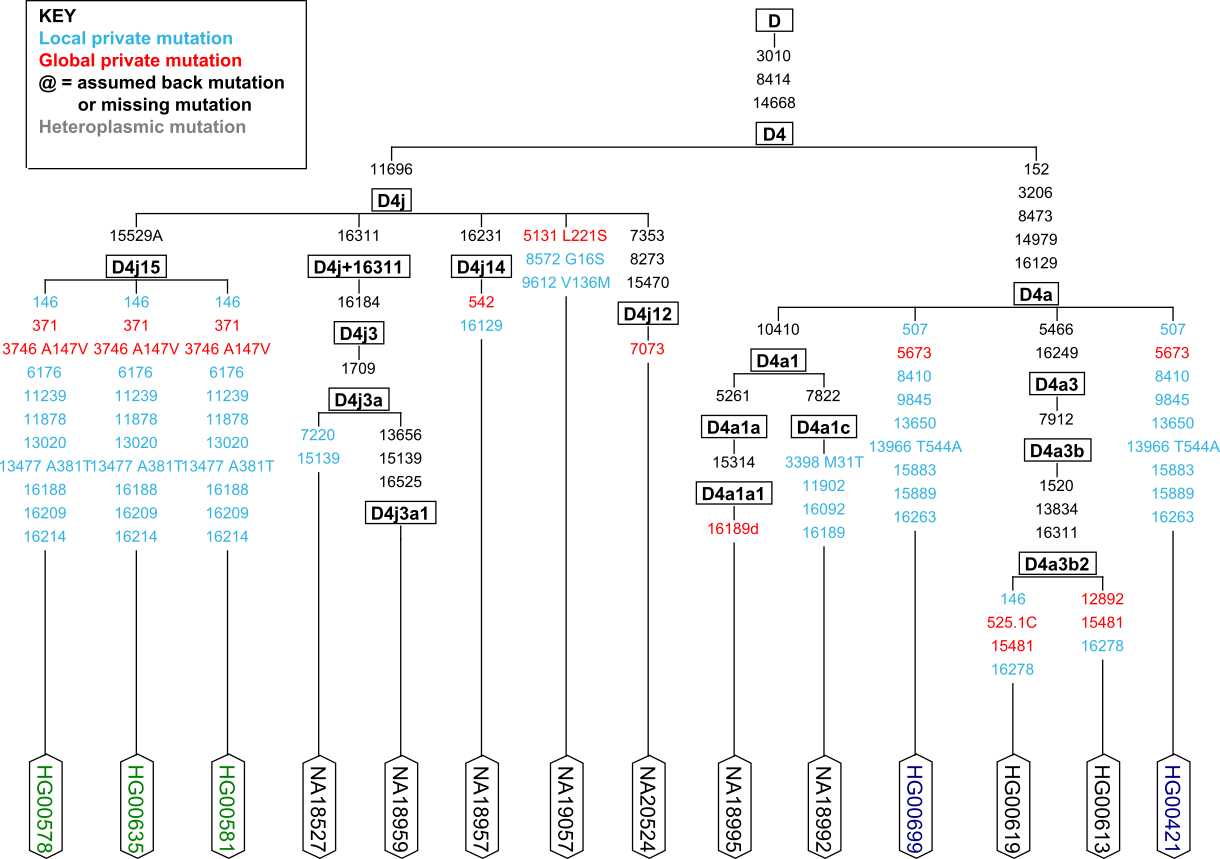
\includegraphics[width=1\textwidth]{images/treeD4.png}
    \caption[Export of Graphical Phylogenetic Tree]{Polymorphisms in the tips of the phylogeny are candidates for new haplogroups, see for instance the samples with green labels belonging to haplogroup D4j15 (confirmed to be related given the sample information provided by the 1000G consortium\footnote{\url{ftp://ftp.1000genomes.ebi.ac.uk/ vol1/ftp/technical/working/20130606\%20sample\%20info/20130606\%20sample\%20info.xlsx}}), or samples HG00699 and HG00421 (not related, marked blue). Polymorphisms marked in red are not occurring in Phylotree and may require additional attention, whereas mutations in blue are private polymorphisms for this group, already known by Phylotree \cite{Weissensteiner2016a}. The annotation of amino acid changes and mutational hotspots (green) are defined by the user itself. Hotspots at positions 16182, 16183 and 16519, AC insertion and deletions at 515–524, inserts at 16193 as well as variation around position 310 and point heteroplasmies can be excluded for the phylogenetic reconstruction. } 
    \label{hg:phylogeneticTree}
\end{figure}
\end{enumerate}

\subsection{Validation Set-Up for HaploGrep}
Since the aim of HaploGrep is to replace a manual process, the results are straight forward to validate. For this purpose, several measurements were taken into account: manually assigned haplogroups from different published studies (see section "Validation Using Predetermined Data" in the HaploGrep paper \cite{Kloss-Brandstatter2011}), were reassigned with HaploGrep and checked for concordance. This process was automated by using the unit testing framework JUnit\footnote{\url{http://junit.org/}}. Thereby these tests validate if HaploGrep results in the expected predetermined haplogroups. These tests are performed with every HaploGrep update. We further compiled a dataset of 120 selected sequences covering the main branches of the human mitochondrial phylogeny (see HaploGrep paper) for test purpose to users, to see the functionality of HaploGrep, without the need of uploading own data. We further checked with the data provided in Bandelt et al. (see Table 2 and Table 3) \cite{Bandelt2012} for the correctness of the haplogroup classification. While the first data set comprises 28 selected control region profiles or partial HVS-I and HVS-II sequence range, the latter represents a dataset of artificially recombined profiles, that should be detected as such. The results of this validation can be found under the Section \ref{hg:qc}.

Additionally the publicly available datasets from the 1000 Genomes Project (1000G) Phase 1 with 1,092 samples and Phase 3 comprising 2,504 samples were used for validation purpose of the different dissimilarity indices, implemented in HaploGrep 2 \cite{Weissensteiner2016a}. The provided information from the consortium are VCF files from both datasets, as well as consensus sequences in FASTA format. The results of the validation are reported in Section \ref{subs:evaluation}. 

\section{Dissimilarity Indices for mtDNA data}\label{hg:dissimilarity}
\label{subs:distance}
 The aim of HaploGrep is to get the best hit from a provided sequence or profile, by comparing it to entries in an in-memory database. Thereby the efficient distance computation is generally an important task in phylogenetics. Knowledge about the mitochondrial phylogeny needs to be taken into account, which limits the usage of ordinary distances. However, distance metrics can often be applied in different scientific areas, as pointed out in the Encyclopedia of Distances \cite{Deza2009}, as for example the Levenshtein metric (or edit distance, Hamming+Gap metric) estimating the costs between strings  \cite{Deza2009}. Therefore, several different dissimilarity indices were taken into account testing accuracy and speed. 
%This section presents the Weighted Hamming distance, provides the introduced Kulczynksi distance for comparison with the Jaccard Indice. The Kimura 2 parameter distance differs in that the information about the substitution rates are weighted based on transition and transversion. This differs from the Jukes and Cantor's model, which assumes independent change with equal probability at all sites. Listed below are the different dissimilarity indices as applied in HaploGrep 2.

\subsection{Weighted Hamming distance}
\label{hamming}
The Hamming distance according Richard Hamming in 1950 adapted here represents the difference between two haplogroups Q and H, where Q is the group of mtSNPs to query and H represents the set of mtSNPs of a haplogroup being an element of the Phylotree (P). Since both strings are aligned to a shared reference sequence R, the length is directly comparable in a compressed bit-mask, where shared elements equal to the reference sequence can be ignored. More formally, the Hamming distance between two haplogroups Q and H is $d_H$ =  $\sum\left|Q_i-H_i\right|$ for all mtSNPs $_i$. The $\min$ $d_H$ $\in$ P represents the best haplogroup match. In order to reflect the human phylogeny, the weighted Hamming distance $d_{Hw}$ is calculated upon the phylogenetic weights presented earlier, instead of the binary mask.
Example: Assume query profile Q = (152C, 263G, 750G, 8860G, 16519) and haplogroup H2 $\in$ P (263G, 750G, 1438G, 4769G, 8860G, 15326G) are compared. 16519 is a mutational hotspot and has weight 0, and is therefore not considered. The resulting bit-mask Q = 11100101 and H2 = 0111110 yields to 
\begin{verbatim}
Q = 152C, 263G, 750G,               8860G,        ->  1110010
H2=       263G, 750G, 1438G, 4769G, 8860G, 15326G ->  0111111
                                                      *  ** *
\end{verbatim}

$d_{H}$ distance 4. Replaced with the phylogenetic weights, the difference $d_{Hw}$ is $|1-0|+|8.8-8.8|+|10-10|+|0-10|+|0-8.8|+|10-10|+|0-10|$ = 29.8 where 10 represents the weight of a mutation with no fluctuation (for mtSNPs 750G, 1438G, 8860G and 15326G), 8.8 represents the weight of two occurrences in P (for mtSNPs 263G and 4769G) and 1 (152C) represents the highest fluctuation rate in P. Therefore this score reflects the phylogenetic distance better than simple counting of differences.

\subsection{Kulczynski Distance}
This distance is the default one applied since the first release of HaploGrep. The details are reported in Section \ref{hg:algorithm}. In order to compare this distance with the Jaccard Index, we here report the same notation, according the sets of mitochondrial profiles $A$, being a subset of all possible base substitutions $P = \left\{ p_1, p_2, ..., p_l \right\} $ with $l$ being the length of the mitochondrial genome, i.e. $l$ = 16569. 
\begin{equation}
d_k (A_1, A_2) = 1 - \frac{1}{2} \left( \frac{\left|A_1  \cap A_2\right| }{\left|A_1  \right|} + \frac{\left|A_1  \cap A_2\right| }{\left|A_2 \right| } \right).
\end{equation}
Again, take the previous example by assuming query profile $A_1$ = (152C, 263G, 750G, 8860G, 16519) and $A_2$ =  (263G, 750G, 1438G, 4769G, 8860G, 15326G) are compared. Again, we replace the polymorphisms with the phylogenetic weight estimated previously and perform the calculation. 16519 is a mutational hotspot and has weight 0.

$d_k$ = 1 - $\frac{1}{2} \left(  \frac{\left| 263G, 750G, 8880G \right|}{\left| 152C, 263G, 750G, 8860G, 16519 \right|} +\frac{\left| 263G, 750G, 8880G \right|}{\left| 263G, 750G, 1438G, 4769G, 8860G, 15326G \right|} \right)$ 
\\= 1 - $\frac{1}{2} \left(  \frac{3}{5} +\frac{3}{6} \right)$ = 0.45

by inserting the weights:
\\= 1 - $\frac{1}{2} \left(  \frac{\left| 8.8 + 10 +10 \right|}{\left| 1 + 8.8 + 10 +10 +0 \right|} +\frac{\left| 8.8 + 10 + 10 \right|}{\left| 8.8 + 10 + 10 + 8.8+ 10 +10 \right|} \right)$ 
\\= 1 - $\frac{1}{2} \left(  \frac{28.8}{29.8} +\frac{28.8}{57.6} \right)$ = 0.266\\
\begin{figure}[!ht]
    \centering
    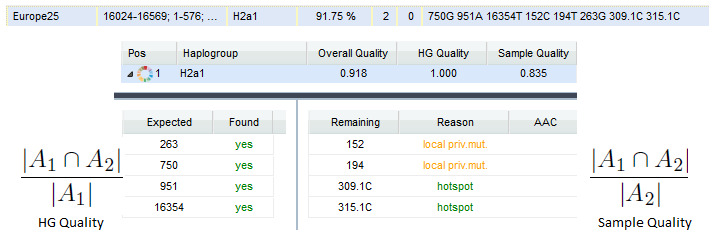
\includegraphics[width=1\textwidth]{images/HG-sample-qual.png}
    \caption[Algorithm's graphical representation in HaploGrep]{ Algorithm's graphical representation in HaploGrep} 
    \label{hg:kulczy}
\end{figure}

It becomes apparent, that the phylogenetic weights yield to a smaller discordance, rendering the two compared haplogroups more similar. The HaploGrep user interface does provide the user the information from both parts of the equation (see Figure \ref{hg:kulczy}), by representing the haplogroup quality (HG Quality) and the sample quality separately as scores, and by listing the polymorphisms in two tabs: expected (all $A_1$ polymorphisms are listed here, with the status found (yes, no)) and the remaining polymorphisms with the status Reason (local private mutation, global private mutation, hotspot or out of range). While out of range, hotspot and global private mutation do not influence the Sample Quality (weight 0), the local private mutation (the mutation has a phylogenetic weight and is observed in other haplogroups). The column AAC indicates the amino acid change for variants in coding regions.  
In the productive version, the results are in the range between $d_k \geq 0.5 $ $ \wedge \leq 1$, where $1$ indicates a perfect match in HaploGrep.

\subsection{Jaccard Index}
According Henning et al. \cite{Hennig2006}, the Jaccard coefficient \cite{Jaccard1901} is presumably the most widely used dissimilarity measure in biogeography. The Jaccard distance is represented by:
\begin{equation}
d_j (A_1, A_2) = 1 -  \frac{\left|A_1  \cap A_2\right| }{\left|A_1 \cup A_2\right|} 
\end{equation}
where $A$ denotes the sets of mitochondrial profiles, and $A_1$, $A_2 \in A$. Again, considering the previous example, the Jaccard distance yields to the result, $d_j$ =
1 - $\left(  \frac{\left| 263G, 750G, 8880G \right|}{\left| 152C, 263G, 750G, 1438G, 4769G 8860G,15326G, 16519 \right|}  \right)$  = 
1 -  $\left(  \frac{3}{8} \right)$ = 0.625. 

By using the weights: \\
= 1 - $\left(  \frac{\left| 8.8 + 10 + 10 \right|}{\left| 1 + 8.8 + 10 + 10 + 8.8 + 10 + 10  + 0 \right|}  \right)$  = 
= 1 -  $\left(  \frac{28.8}{58.6} \right)$ = 0.509. 
\subsection{Kimura - two parameter model}
One of the most widely used evolutionary distance, i.e. a model of DNA evolution is the Kimura two parameter model. The frequency matrix for a base exchange according Kimura \cite{Kimura1980} is based on the transitions (A $\leftrightarrow$ G and C $\leftrightarrow$ T) and transversions (all other base exchanges from pyrimidine to purine and vice versa). This differs from the Jukes and Cantor's model, which assumes independent change with equal probability at all sites.
Table \ref{hg:kimuratable} indicates the base substitution as transition (denoted as $\alpha$) and transversion (denoted as $\beta$). Thereby the model assumes an equal distribution of all nucleotides ($\pi$A = $\pi$C = $\pi$G = $\pi$T = 0.25 $\mathcal{N}$). Based on the rCRS, this is however not the case for the mitochondrial genome ( $\pi$A = 0.309 $\pi$C= 0.313 $\pi$G=0.131$\pi$T=0.247).
\begin{table}[h]

\centering
\caption{Rate matrix of the transition states of nucleotide bases: transitions ($\alpha$) and transversions ($\beta$) for the Kimura 2 parameter model.}
\label{hg:kimuratable}
\begin{tabular}{lllll}
\hline
   & A&  C   &G  & T\\
\hline

A  & - & $\beta$    & $\alpha$  & $\beta$ \\
C  & $\beta$ &  -   & $\beta$  & $\alpha$ \\
G  & $\alpha$ &  $\beta$    & - & $\beta$ \\
T  & $\beta$ &  $\alpha$    & $\beta$  & - \\
\end{tabular}
\end{table}

The Kimura two parameter distance, called K80 model (based on the year of publication), is calculated by:
\begin{equation}
K80 = - \frac{1}{2} \log((1- 2p -q ) \sqrt[]{1-2q})
\end{equation}
where the two parameters $p$ and $q$ represent the proportion of sites that show transitions and transversion respectively.

In the mitochondrial DNA the occurrence of a transition is 20 times more likely than a transversion (for homoplasmic SNPs \cite{Guo2012}). Based on our analysis of the 1000G Phase 3 mitochondrial genomes, this Transition / Transversion ratio $k$ can be confirmed, varying between $k=1:17$ and $k=1:30$ depending on the reference sequence. By considering only the heteroplasmic variants in the 1000G phase 3 data set, the ratio is $k=$ \textbf{1:21}. For the nuclear DNA, the Transition / Transversion ratio assumes transitional changes about four times more likely than transversional changes \cite{salemi2009the}. 


\subsection{Evaluation}
\label{subs:evaluation}

For validation purposes we applied all four presented distances to the 1000G Phase 1 data (n=1,074) as well as to the dataset provided by Li et al. \cite{Li2014}, including 2,000 exome sequencing mtDNA data from a Danish cohort. Table \ref{table:distances} presents the summary of the evaluation. The entries in the upper triangular matrix are the percentage of identical haplogroup results between the different algorithms. Haplogroups using any “+” notation with the same slot were not considered, since MitoTool is not supporting such groups (accounts for 66 to 69 haplogroups, depending on the HaploGrep 2 algorithm used). The detailed results are provided in Supplemental Material of the HaploGrep 2 publication\footnote{\url{http://nar.oxfordjournals.org/content/suppl/2016/04/15/gkw233.DC1/HaploGrep2-SupplementalMaterial.pdf}}. 
\begin{table}[H]
\centering
\begin{tabular}{l|l|llll}
\cline{3-6}
 &    & \multicolumn{4}{c|}{HaploGrep} \\ \hline
\cellcolor[HTML]{FFFFFF} & \cellcolor[HTML]{FFFFFF} & \cellcolor[HTML]{FFFFFF}Hamming & Kulczynski & Jaccard & Kimura2P \\
MitoTool & & \multicolumn{1}{c}{\cellcolor[HTML]{96FFFB}96.84} & \multicolumn{1}{c}{\cellcolor[HTML]{96FFFB}96.65} & 
\cellcolor[HTML]{96FFFB}96.75 & \cellcolor[HTML]{96FFFB}96.75 \\ \hline
HaploGrep & Hamming & \multicolumn{1}{c}{\cellcolor[HTML]{FFFFFF}{\color[HTML]{330001} }} & \multicolumn{1}{c}{\cellcolor[HTML]{A9D0FF}98.98} & \cellcolor[HTML]{34CDF9}99.54 & \cellcolor[HTML]{ECF4FF}95.82 \\
HaploGrep  & Kulczynski & & \cellcolor[HTML]{FFFFFF} & \cellcolor[HTML]{A9D0FF}98.88 & \cellcolor[HTML]{96FFFB}96.28 \\
HaploGrep & Jaccard & & & & \cellcolor[HTML]{ECF4FF}95.72 \\
HaploGrep & Kimura2P & & & & \cellcolor[HTML]{FFFFFF} \\
\end{tabular}
\caption{Comparison of MitoTool and HaploGrep 2 with the extended dissimilarity indices in regard of the 1000G phase 1 data (n=1,076).}
\label{table:distances}
\end{table}
While the run-time of the first three distances was almost identical (see Table \ref{table:speed} for details) with 4.6 – 4.7 sec, the Kimura2P distance showed a 33-fold higher wall-time (158.1 sec). The ratio was similar for the Li data
(6.4 sec for Kulczynksi vs. 210 sec for Kimura2P). With the different results in 21 out of the 1,074
samples (1.96\%) in the 1000G phase 1 data, 153 out of 2,534 (6.11\%) in the 1000G phase 3 data
and 98 (4.9\%) out of 2,000 in the exome sequencing samples, the user gets additional informations
about the data quality and can check the corresponding samples. The varying coverage in the exome data and problems with the VCF file in the 1000G phase 3 data become apparent (see Table 1
and Supplemental Material Table 2 - 4) \cite{Weissensteiner2016a}. We therefore provide this combined haplogroup estimation
mode (Button “Haplogroup Discordance Check”), which lists all samples where at least one metric
yields a different result \cite{Weissensteiner2016a}.

\begin{table}[H]
\centering

\begin{tabular}{|l|l|l|l|l|l|}
\hline
              & MitoTool  & Hamming  & Kulczynski & Jaccard  & Kimura2P   \\ \hline
1000G phase 1$^{1}$ & 177.3 sec & 4.7 sec  & 4.6 sec    & 4.7 sec  & 158.1 sec  \\ \hline
Danish Cohort$^{2}$ & 447.6 sec & 6.42 sec & 6.37 sec   & 6.39 sec & 210.97 sec \\ \hline
\end{tabular}
\caption{Wall time of haplogrouping classification over different methods, on 1,074$^{1}$ and 2,000$^{2}$ samples in form of hsd variant files - no sequence alignment required. }
\label{table:speed}
\end{table}



\section{Quality Control}\label{hg:qc}
One of the main importance of the haplogroup classification results from the knowledge about mutations which are expected in a specific haplogroup, and about those who are not observed in the haplogroup or even in the current phylogenetic tree. Based on this knowledge, several means for quality control of mtDNA data can be applied as presented in this Section.
\subsection{Artificial recombination detection}
The 16,6 kilobases of the mitochondrial DNA are chopped in smaller fragments when sequenced for being amplified with the polymerase chain reaction (PCR). This means that multiple fragments of one sample are sequenced. For the whole mitochondrial genome, usually 2 fragments (also 1 long range possible) are needed, each comprising between 8kb and 10kb. Different protocols exist, which use 3 or more fragments. Since several manual steps are required when handling the sample in the lab, a fragment could be switched between samples - resulting in so called artificial recombination. Issues with fragments in an NGS sequencing project where the wrong amplification of fragments was applied due to switched concentration in the sample preparation step can occur.
To check for issues with fragments, derived from different samples, a module \textit{"Check for Recombination"} was implemented in HaploGrep. The algorithm for this procedure is  drafted as presented in algorithm \ref{algRecomb1}, on a per sample basis.
\begin{algorithm}
  \caption{Estimation of artificial recombinants}
  \label{algRecomb1}

Estimate the haplogroup $H$ of the complete provided mitochondrial profile 

Split the sample profile according the fragments $F$ used, and estimate the haplogroup per fragment ($P_{f_i}$)

Split the reference haplogroup $H$ profile according the fragments $F$ and estimate the haplogroup per fragment ($R_{f_i}$)
	
For each fragment compare the phylogenetic distance $\gamma_f(i)$ of the resulting haplogroup and calculate the total score 
$\sum_{n=1}^{length(f)} |{\gamma_f(P_{f_i} - R_{f_i})| > 5}$ 
where all samples with distances in the phylogenetic Tree surpassing five nodes are emitted as potentially recombinant.
\end{algorithm}


 
As a second approach for detecting artificial recombination, the method described in Kong et al. \cite{Kong2008} for checking constituents in a sample mix-up was implemented. The basic concept here is to estimate the haplogroup of a sample in a first iteration, similar as in the previous described approach. In a second iteration, all mitochondrial polymorphisms, that could not be assigned to the best resulting group are used to make up a new virtual profile. These secondary possible constituents are affiliated to haplogroups and the number of haplogroup defining constituents confirms the possible contamination. The two steps of the algorithm can be drafted as follows:
\begin{algorithm}
  \caption{Steps for recombination check adapted from Kong et al.}
  \label{algRecomb2}
Primary Classification: Estimate the haplogroup $H$ of the complete provided mitochondrial profile. 

Secondary Classification: For all mutations $m$ not being covered for the primary classification, the haplogroup with the least difference to the rCRS is estimated. If the resulting haplogroups differs from H2a2a1 and the elements in $m$ are not phylogenetic hotspots, a warning for possible contamination is emitted.
\end{algorithm}

Given the dataset in Bandelt et al. \cite{Bandelt2012}, the herein described methods were assessed for reliability. In the first paper, describing the haplogrouping classification, these recombinations remained undetected by HaploGrep, which could be seen as a limitation. The check for remaining variants was able to detect six out of the seven cases, while the fragment-based check could reliably detect all samples as artificial recombinants. Table \ref{table:recomb} lists the results of the two methods presented in Algorithm \ref{algRecomb1} and Algorithm \ref{algRecomb2}, by extending the table provided by Bandelt et al. \cite{Bandelt2012}. 


\begin{table}[H]
\centering

\begin{tabular}{lllll}
ID & HG Status & Exp. vs. Est. & Algorithm 4 & Algorithm 5\\ \midrule
USA.AFR.942 & L1b$|$C1 & C1c$|$X M31a1 & L1b$|$C1 &  M31a1$|$L1b3 \\
FRA.CAU.84 & HV0$|$J1c & ?$|$? & HV0$|$J1c2 & J1c2 \\
VP61 & T2b$|$J1b1a & T2b$|$T U5 & U5b3h$|$J1b1a & T$|$U5a1d2b \\
739 & B4a$|$B4b1a1 & M7c$|$R30a & D5c1a$|$B4b1a1 & R31$|$B4b1a1 \\
92 & B4b1a1$|$B5b & B4b1$|$B4b1& B4b1a1$|$U6a2 & B4$|$B4b1a1c \\
LPAZ092 & B2$|$C1 & B4$|$?& B4 B2$|$C1 & B4$|$C1b14 \\
LPAZ094 & C1$|$B2&U5b2a1 M8& C1$|$H1a & C4a2a$|$M80 
\end{tabular}
\caption{Artificial Recombination: HG Status is according Phylotree 13 while Results from the herein described Algorithm   \ref{algRecomb1} (fragment based check) and Algorithm \ref{algRecomb2} (the method according Kong) were performed on the latest Phylotree version 17.}
\label{table:recomb}
\end{table}

\subsection{Phantom mutation detection}
\label{hg:phantom}
Systemic artefacts either generated during the sequencing process itself or the computational post-processing steps are denoted as phantom mutation. In order to identify such potential phantom mutations, requiring closer examination, phylogenetic knowledge can be exploited. Two main approaches for identifying patterns of phantom mutation are presented in this regard: Median networks and screening for rare mutations in order to see whether mutations occur in more than one haplogroup. Furthermore checks for several known phantom mutations can be applied. 

HaploGrep supports the generation of \textbf{Quasi-median Networks} by generating files for the phylogenetic application Network 5. The application generates visualizations of evolutionary trees and networks, and is not limited to genetics, but can also be applied in linguistics. The concept here is to check the data table of the differences in the mtDNA sequences for pairwise compatibility. 

A second method is focused on the \textbf{rare mutations} in samples, not being assigned to haplogroups. Thereby the underlying dataset is crucial for this task. The current worldwide database for mitochondrial DNA sequences GenBank\footnote{\url{http://www.ncbi.nlm.nih.gov/genbank/}} hosts over 31,000 full human mitochondrial DNA sequences, as of March 2016. However issues with the quality in this public dataset were already shown by Yao et al. in 2009, when GenBank contained 6,700 complete mtDNA genomes \cite{Yao2009}. While we compiled a dataset of 30,500 full mtDNA genome sequences derived from GenBank mtDNA Sequence Checker from Ian Logan\footnote{\url{http://www.ianlogan.co.uk/checker/genbank.htm}} as of October 2015. By calculating the fluctuation rates per position over all samples we compared the score to the very well curated data set from Soares et al. \cite{Soares2009}, comprising 2,196 full mitochondrial genomes. When considering only positions occurring in both data sets, a regression analysis showed a correlation coefficient of 0.68 over 3,356 sites with a standard error of 0.002 and with a p-value of $1.28^{-9}$ in the mutation rates between the two data sets. When excluding mutation on 310T$>$C, the correlation coefficient increases to 0.95 in 3,355 observations, while the standard-error decreases to 0.0007 and the p-value to $2.6^{-42}$. Based on these findings the large data set results as suitable to be used as database to check mutations for the occurrence. While in the Soares data set, known phantom mutations are present with a score up to value 2, in the new distilled data set, a filter on undefined nucleotides N as well as heteroplasmic positions was applied. Further the presence of  at least 4 occurrences of a mutation in the list was applied. The resulting hash-map (with key being the variant and value the amount of recurrence in the data set) contains 4,010 entries. 
For all polymorphisms which are remaining after haplogroup classification the presence in this distilled list is checked. If a mutation is not present in the hash-map, and at least two samples in the investigated population show the mutation, it is reported as a potential phantom mutation. Further a check for known phantom mutations described in the literature is performed \cite{Brandstatter2005,Bandelt2002}. The resulting list of phantom mutations is sorted according the number of occurrence in the uploaded data set, by providing the sample ids. By checking large data sets like the data from 1000G, issues with data quality becomes apparent.

\subsection{Dissimilarity indices concordance }
By validating the previously presented dissimilarity metrics in terms of speed and accuracy, the Kulczynski distance showed the best performance. However, in some cases where the profile is close to the root of the phylogenetic tree, or where transversions are present, the Hamming Distance and the Kimura-2P distance respectively, estimate alternative haplogroups that need to be re-checked by the user. But also the Jaccard distance, having the highest similarity to the Kulczynski distance, can yield in some special cases to different best haplogroup results that need consideration by the user. To allow this operation, an automatic check for haplogroup concordance is directly implemented in HaploGrep, where for each metric, the best 5 haplogroup hits are calculated and the resulting sets are compared for intersections. A list of samples with discordant results is emitted subsequently. 

\section{MultiMap: Optimizations for MicroArray data}\label{hg:optimization}
The current version of HaploGrep 2 accepts data generated by different genotyping DNA Chips (MicroArrays), in the form of VCF or hsd files (see Section \ref{hg:input}), however the computation-time decreases with the increasing amount of genotypes, each handled by providing an element of a range array. This is required, to not interpret not examined genotypes falsely as back-mutations. Thus, the comparison for the presence in the given input-range requires additional computation time and slows down the process of haplogroup classification, when considering thousands of samples where only specific genotypes are present. To overcome this limitation, a new classifier is introduced, in this section. 
\subsection{Algorithms}
The foundation of the optimized version, is the use of an Key-Value approach based on the recursive function presented in Section \ref{hg:algorithm}, that is used to write the \texttt{key} = haplogroup, and the \texttt{value} = list of polymorphisms defining the haplogroup. Thereafter an inverted index is created, consisting of the list of all unique polymorphisms occurring on Phylotree, by providing for each polymorphism a collection of haplogroups in which it appears. This allows the quick search for profiles by using a map that holds a collection of values against each key. Here the Google Guava Multimap framework \footnote{\url{https://github.com/google/guava/wiki/NewCollectionTypesExplained}}, was considered.
%While \texttt{HashMap<K, ArrayList<V>>} can be used in Java, to associate arbitrarily many values to a key, here the Google Guava Multimap framework \footnote{\url{https://github.com/google/guava/wiki/NewCollectionTypesExplained}}, was considered. The Apache Commons Collection also provides a MultiValuedMap\footnote{\url{https://commons.apache.org/proper/commons-collections/apidocs/org/apache/commons/collections4/MultiValuedMap.html}}, so that programmers don't not need to reinvent the wheel, when working with this abstract data structure.

The resulting algorithm for estimating the haplogroup from a query profile $Q  = \left(q_1,q_2,\dotsc,q_n\right)$, with $q_i \in P$, where $P$ represents the set of all polymorphisms contained in Phylotree and $_i$ the length of the query profile $|Q|$ is a distance maximizing problem. By iterating over the query profiles $q_i$ for each list of values, the haplogroups $H \left(h_1,h_2,\dotsc,h_n\right) \in$ Phylotree, with $n$ the number of elements of haplogroups present in Phylotree, are added to a new resulting HashMap $R$, where the key $rk = h_j$ and the value $rv$ = the phylogenetic weight $w_i$ for the polymorphism $q_i$ and $w_i = \left[1, 10\right]$. The key with the highest value and the least remaining SNPs represents the result = $ \min\left(\max\left(rv\right)\right)$. 
As an example, consider the query profile $Q$ with 4 mtSNPS  1438G, 3010A, 8860G, 15326G. By iterating over the MultiMap index, with Key = mtSNP and values being the haplogroups that contain the mtSNP, for each haplogroup represented in Phylotree the sum of the scores of the wights is estimated. For those haplogroups with the highest such score, the one with the least additional SNPs is calculated. If there's only one haplogroup left for assignment, this is the result, otherwise the cluster of haplogroups fulfilling the requirements is emitted as result.

\subsection{Performance Validation}
Based on different data sets (e.g. from the 1000G Phase 1 data set and the Danish cohort presented earlier (see Evaluation \ref{subs:evaluation}), as well as publicly available data from GenBank), the haplogroup classification in HaploGrep 2 is reassessed and compared to the previous version and the MultiMap version. 
\begin{enumerate}[label=(\alph*)]
\item  the full input range (i.e. 1-16569)
\begin{table}[H]
\centering
\caption{Runtime of different methods}
\label{hg:runtime1}
\begin{tabular}{|l|l|l|l|l|}
\hline
             & Samples & HaploGrep & HaploGrep 2 & Multimap \\ \hline
1. 1000G P1  & 1,074   & 37  & 5.23        & 4.97         \\ \hline
2. 2K Danish & 2,000   & 73 & 7.45       & 6.83        \\ \hline
3. 1000G P3  & 2,534   & 92 & 11.31      & 10.9         \\ \hline
4. merged 2 + 3 & 4,534   & 162 & 18.22       & 17.04        \\ \hline
5. GenBank* & 10,000   & 353 & 48.3       & 43.12         \\ \hline
6. GenBank*  & 20,000   & NA & 95.69       & 80.89         \\ \hline
7. GenBank*  & 30,561   & NA & 138.47      & 125.2        \\ \hline
\end{tabular}
\end{table}

\begin{figure}[!ht]
    \centering
    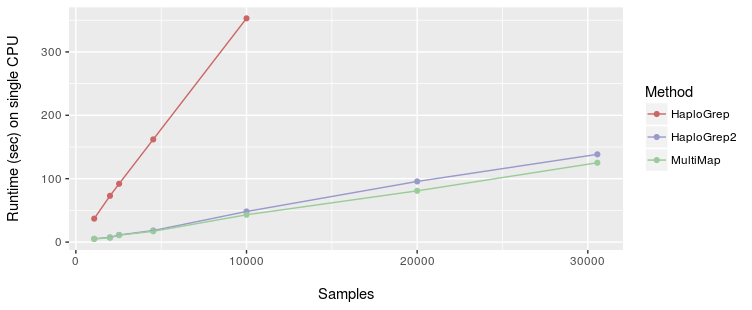
\includegraphics[width=1\textwidth]{images/multimap.png}
    \caption[Run time comparison of HaploGrep versions]{Run time comparison of full range sequences with different methods HaploGrep, HaploGrep2 and the Multimap approach} 
    \label{hg:mutlimap}
\end{figure}

\item  the input range as a semicolon separated list (e.g. 64;73;93;...), by including all polymorphisms in the samples. 

\begin{table}[H]
\centering
\caption{Comparison of different MicroArrays}
\label{hg:}
\begin{tabular}{ll|l|l|l|l|}
\cline{3-6}
                               & Samples & \multicolumn{2}{l|}{1000G P1 (n=1,074)} & \multicolumn{2}{l|}{GenBank* (n=12,503)} \\ \hline
\multicolumn{1}{|l|}{}         & mtSNPs  & HG2               & Multimap            & HG2              & Multimap           \\ \hline
\multicolumn{1}{|l|}{Illumina} & 226     & 9.94              & 2.76                & 104.19           & 26.54              \\ \hline
\multicolumn{1}{|l|}{Affy 6}   & 454     & 14.56             & 4.06                & 182.03           & 40.99              \\ \hline
\multicolumn{1}{|l|}{23andMe}  & 3,154   & 65.4              & 5.05                & 775.92           &       47.27             \\ \hline
\end{tabular}
\end{table}
\begin{figure}[!ht]
    \centering
    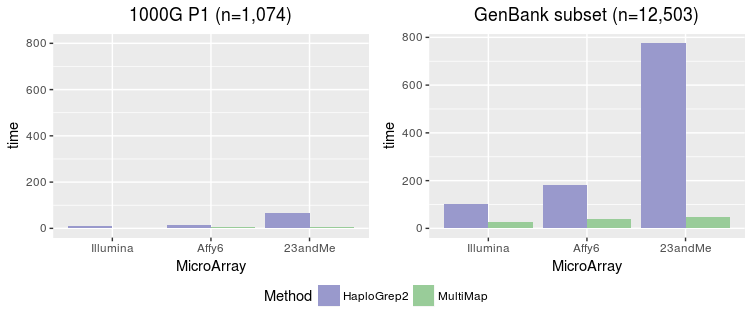
\includegraphics[width=1\textwidth]{images/multimap2.png}
    \caption[Run time (in sec) comparison of HaploGrep versions]{Run time (in sec) comparison of different MicroArrays. HG2 represents the HaploGrep 2 algorithm, Multimap the optimized hash based approach} 
    \label{hg:multimap2}
\end{figure}
\end{enumerate}

The updated version HaploGrep 2 could be improved by a factor of $\sim$ 8 fold to the first version of HaploGrep (see Table \ref{hg:runtime1} and Figure \ref{hg:mutlimap}. While the underlying tree increased significantly from 2,128 nodes to currently 5,435, the improvement between the two versions is by a factor of $\sim$ 15. This is partly the result of in-memory optimization, by reducing the list of the best hits with the corresponding trees stored for each sample. 

The evaluation shows that the improvement for whole mitochondrial genome sequences are marginal, but are essential for large studies with MicroArrays. The runtime were on one single CPU only, therefore taking advantage of current multi-core architectures, additional speedup can be achieved. 

\section{Conclusion and Outlook}\label{hg:outlook}
In this chapter, an algorithm and its implementation called HaploGrep were described. It is designed to assign haplogroups to given mitochondrial profiles to be examined. This is of special interest in various genetic fields, and will become of interest to a broader spectrum of users in the near future. The increase of personal genetic testing companies like 23andMe, ancestry.com, Living DNA, Family Tree DNA, or the National Geographic Genographic Project to name the most prominent as of 2017, already bring this information directly to the customers. These are currently limited to the ancestry aspect. Haplogroups provide a coarse information in this regard (based on the mutation rate of one fixed mutation in every $\sim$ 3,000 years). Haplogroups will also gain on importance for mitochondrial replacement therapy, where a haplogroup matching between donor and recipient is highly suggested \cite{Royrvik2016}, highlighting the importance of accurate haplogroup estimation. Different tools as well as distance measures where compared regarding their performance and evaluated in this chapter, by showing that the implementation in HaploGrep outperforms current available tools, in terms of accuracy and speed. The run-time can be optimized with hash-based data structures and the use of an inverted index, especially for MicroArray data. Further improvements can be a pre-classification based on sub-setting the phylogenetic tree, of the main branches, comprising a small amount of nodes $n$, where $n = 25$ based on the current phylogenetic data \cite{VanOven2015}. Thereafter the subbranches of the node with the highest score needs to be performed. By introducing this group-based layer, the haplogroup calculation can be reduced to a lower-dimensional space. A further problem is the generation of the underlying phylogenetic tree, currently performed in a mostly manual way. By generating Maximum Parsimony Trees based on mtphyl\ref{mtphyl} that need to be confirmed by at least two independently sequenced mitochondrial profiles, the world-wide mtDNA phylogeny is currently curated by Mannis van Oven \cite{VanOven2015} in cooperation with the Forensics Institute of Innsbruck in a semi-automated way. While HaploGrep already takes advantage of XML-structured tree, an extension to allow the addition of nodes directly in this tree are not of technical limitation, and could refer to the growing amount of world-wide available mitochondrial full genome sequences, currently from 32,000 to millions in the next years.

\cleardoublepage
\chapter{Algorithms and Data Structures for mtDNA Sequence Alignment}
\label{chapterAlignment}
\label{chap:alignment}
The algorithm of life is based on a set of building blocks, that are passed on to the next generation, based on the concept of enormous redundancy \cite{DO90}. Thereby the concept of evolution is based on reusing and modifying successful sequences or structures. Genes working in fruit flies are highly similar to those working in humans, features that are associated with mtDNA mutations in vertebrates are conserved in fruit flies with comparable somatic mtDNA mutation frequency (${\sim 10})^{-5}$) \cite{Itsara2014}. However both species do differ significantly from each other. While redundancy and similarity play an important role, the differences and conservation between sequences (encoding complex structures and mechanisms) are essential. To make any statements about the differences, various different sequences need to be aligned. The alignment of sequences is thereby one of the most central problems in the field of computational biology. Performing an alignment allows to detect and compare mutations, so called single nucleotide variants or polymorphisms, as well as short insertions and deletions (indels), being essential for DNA, RNA or amino acid sequence interpretation \cite{Gusfield1997}. According to Gusfield, high sequence similarity implies functional or structural similarity.  
\iffalse
Besides Next-Generation Sequencing devices distributing rapidly in the labs around the globe, Sanger sequencing is still used in Labs for DNA sequencing\footnote{https://www.lifetechnologies.com/at/en/home/life-science/sequencing/sanger-sequencing.html}. It is the workhorse that made it possible to determine the complete sequence of roughly 3.2 billion bases of the human genome in a time span of 13 years. Thereby it is very accurate, with fewer than one error per 10,000 bases\footnote{http://www.genome.gov/11006929}, corresponding a Phred quality score of $\geq$ 40. Most NGS devices show an error per base rate of Phred quality score 30 or below, third generation devices like the Oxford Nanopore show sequencing errors with Phred quality scores ~10 \cite{Ip2015} (indicating 10 errors on 100 basepairs), however yielding long reads of several kilobases. 
\fi

As abstracted in the introduction (Chapter \ref{chapterIntro}), different methods do exist to read out DNA and RNA sequences. Thereby the data generated by the sequencing devices comes as sequences of the alphabet set \(\{A, C, G, T\}\) whereby some special characters are used such as \textit{:} or \textit{d} representing one deleted base, - representing deleted base of unknown length, \textit{N} for any base, \textit{R} for purine (A or G), \textit{Y} for pyrimidine (C or T) called heteroplasmic mutations. The base sequence is essential, but gains even more importance if it can be compared to other sequences. So, having obtained the consensus sequence with one of the different ways of date generation in the lab, the issue now is to compare those sequences. This is of great importance in the field of phylogeny and evolution, but is also applied in gene discovery and detection of function of proteins to already known domains. This Chapter therefore gives an overview on this central problem in bioinformatics: sequence alignment, by focusing on the short circular mitochondrial genome sequence. The problem of alignment here is that a software generates only one of many possible representations. Different interpretation of insertion, deletions or transition / transversion can results to different nomenclature, limiting the interpretation and in the worst case resulting in wrong statements about pathogenic mutations or the misidentification of criminals (like the misidentification of Jack the Ripper\footnote{\url{http://www.independent.co.uk/news/science/jack-the-ripper-id-hinges-on-a-decimal-point-as-scientists-flag-up-dna-error-in-book-that-claims-to-9804325.html}} where we raised concerns about the correctness of the data). To prevent such a misinterpretation the concept of a recommendation system, based on a larger reference panel is introduced, and implemented as part of the HaploGrep system. Prior to that, this chapter gives the background of the alignment problem, with solutions and validation of related methods.

\section{Background: Mind the gap}
The alignment of two sequences $S_1$ and $S_2$ $\in \{A,C,G,T,N\}*$ (where $N$ is a placeholder for $A, T, G,$ or $C$) is a computation problem with complexity $\mathcal{O}(n \times m)$, where n =length $S_1$ and m= length $S_1$. For pairwise comparison of mitochondrial genomes, this corresponds $\mathcal{O}({n}^{2})$. For aligning $S_1$ and $S_2$, ${{n+m}\choose{m}} \sim \frac{ {2}^{m  + n}}{\sqrt[]{\pi m}}$   \footnote{\url{http://www.cs.columbia.edu/4761/notes07/chapter2.1-Alignment.pdf}} different possible alignments can exist. However only a small subset of all possible alignments are biologically meaningful. To weight the different alignments, the simplest form would be to use the Hamming Distance (see \ref{hamming} and count the mismatches between two sequences D($S_1$,$S_2$). However the differences between two nucleotide sequences are not just single nucleotide variants, but can be present as insertions and deletions, rendering the Hamming Distance in this context merely useless. Also, the sequences can be of different length, being of requirement for the calculation of this distance. To cope with the gaps in form of insertions and deletions, the Levenshtein-distance, (often referred to as edit distance, shuffle-Hamming distance or Hamming+Gap metric) \cite{Deza2009} was introduced in 1965. It is based on a set of edit operations - copy or match (M), substitute or replace (R), insert (I) and delete (D). Thereby this operations build a string over the alphabet (M, R, I, D), describing the transcript from one sequence to the other (see Gusfield Chapter 11) \cite{Gusfield1997}, where the operations can have different weights ($w_M$=0, $w_I$=1, $w_D$=1, $w_M$=1). The following listing represents the transcript string between the sequences $S_1$ = ATCAGACGAG and $S_2$ ACAGGCGAT:
\begin{center}
\texttt{ATCAGACGA G} \\
\texttt{A CAGGCGATG} \\
\texttt{-----------} \\
\texttt{MIMMMRMMMDM} \\
\texttt{01000100010} \\
\end{center}
The edit distance is the minimum number of weights (i.e. edit operations, for all replace, insert and delete operations). This approach is part of inexact string matching class (see \ref{inexact}). Alternatively exact string matching approaches do exist, that are outlined in the subsequent section \ref{exact}. 

\subsection{Exact String Matching}
\label{exact}
The problem of exact string matching, is to find all occurrences of a string $P$ called \textit{pattern} and $T$ called the \textit{text}, by exactly finding the pattern $P$ as substring of $T$. While this might sound like an simple problem, the worst case running time for the naive method is $\mathcal{O}({n}\times{m})$ where $n$ denotes the length of $P$ and $m$ denotes the length of the text $T$.
\subsubsection{Naive Algorithm}
The naive algorithm takes the text $T$ and the patterns and $P$ as input by checking for each sequence of length $i = 1, 2, 3, \cdots m-n+ 1 $ if a substring in T can be found such that $t_i \cdots t_i+m = P$. This approach can be reduced to $\mathcal{O}({n}+{m})$
\subsubsection{Boyer-Moore Algorithm}
The Boyer-Moore Algorithm is an extension of the naive algorithm, based on 3 different rules, which improve the runtime significantly. 
\begin{itemize}
\item[1] \textbf{right to left scan in $P$}, which is not an optimization per se, but is used for the both rules, 2 and 3. 
\item[2] \textbf{bad character shift rule}: start with comparing pattern $P$ with text $T$ from left to right, while applying rule 1 for pairwise comparison of $P$ and $T$. Until a mismatch happens, compare $P_i$ with $T_{|P_i|}$, with i $\in (0,\cdots |P|)$ . If mismatch occurs, skip alignment until the next character in $P$ matches the mismatch on $T$ or skip the complete P and proceed on $T_{|P_i|}$. Figure \ref{fig:boyer2} represents the rules 1 (green arrow scanning right to left), and the 2 mismatches for the bad character shift rule.
\begin{figure}[!ht]
\label{fig:boyer2}
    \centering
    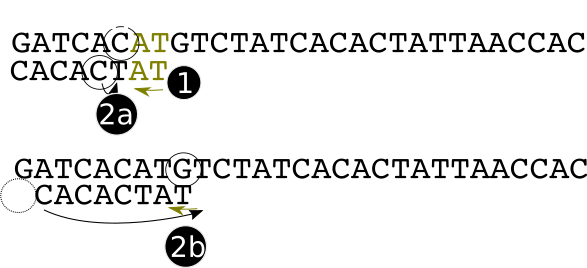
\includegraphics[width=0.6\textwidth]{images/boyer2.png}
    \caption[Boyer-Moore - example rule 1 and 2]{Boyer-Moore - example for rule 1 and 2. Pattern $P$ = \texttt{CACACTAT} is scanned from right to left. In 2a, a mismatch in the Text on position 3 happens. Subsequently $P$ is shifted for the next C, so that it matches with this position. Since in 2b no G can be found in the $P$, the complete string can be shifted behind this position on the text $T$.} 

\end{figure}

\item[3] \textbf{good suffix shift rule} This rule checks if a suffix from right appears subsequently after a mismatch. If the suffix $t$ can be found in $P$, alignments can be skipped and $P$ shifted - see Figure \ref{fig:boyer3} for an example.
\begin{figure}[!ht]
\label{fig:boyer3}
    \centering
    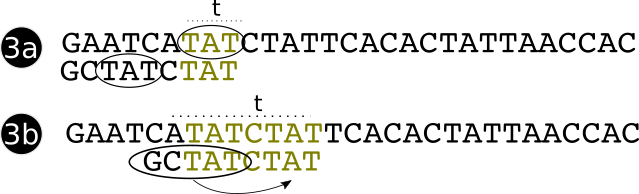
\includegraphics[width=0.65\textwidth]{images/boyer3.png}
    \caption[Boyer-Moore - example rule 3]{Boyer-Moore - example for rule 3. Subpattern $t$ = \texttt{TAT} is matches as suffix, and is 3 bases long, until a mismatch happens. Thereafter, good suffix is searched in $P$ with less search effort (3a). A suffix can also be repetitive, so that the the repetition skips alignments, by shifting to the first presence of In 2a, a mismatch in the Text on position 3 happens. Subsequently $P$ is shifted for the next C, so that it matches with this position. Since in 2b for the $P$ no G can be found, the complete string can be shifted behind this position on the text $T$.}
\end{figure}
\end{itemize}
The algorithm performs both rules and decides on the one that skips more alignment steps. A further step is the creation of a lookup table, where the number of skips are precalculated based on $P$. There do exist some more algorithms for exact string matching like the Knuth-Morris-Pratt algorithm or the 
\subsubsection{Offline Algorithm}
While the previously described naive algorithm and its optimization the Boyer-More algorithm, represents so called online algorithms (processing without an index), there is a second class of algorithms, based on the concept of preprocessing of the text $T$, and based on index. While this preprocessing step takes additional time and space, the overall runtime can be reduced significantly. Offline algorithms are also implemented in most modern web search engines.  The most notable offline algorithms are  k-mer or n-gram based search, suffix trees or metric trees. Since used in the subsequent sections, k-mer and suffix trees are shortly outlined within this paragraph.
\begin{itemize}
\item \textbf{k-mer} or \textbf{n-gram}: here the \textbf{k} or the \textbf{n} stand for the length of substrings of all possible occurrences in the text $T$. Figure k-mer gives an example with the text $T$ = \texttt{GAATGAATGC}, resulting in the sorted index. The lookup is often implemented as a HashMap, so that the generation of the index is $\mathcal{O}({n})$ and the query $\mathcal{O}({1})$
\begin{figure}[!ht]
\label{fig:k-mer}
    \centering
    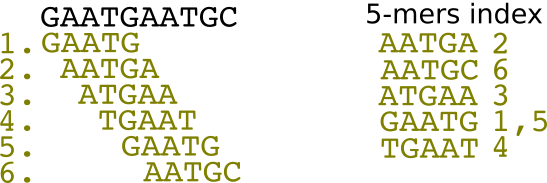
\includegraphics[width=0.65\textwidth]{images/k-mer.png}
    \caption[k-mer or n-gram]{k-mer or n-gram applied to the text  $T$ = \texttt{GAATGAATGC}. The k here is of length 5, so the index represents all possible 5-mers or 5-grams occurring in $T$. If for one entry, multiple positions in $T$ are be found (see \texttt{GAATG}, which starts on position 1 and 5), a Multimap can be used.}
\end{figure}
\item \textbf{Suffix-Tree}
Suffix Trees are a very efficient data structures, to perform the exact string matching in linear time $\mathcal{O}({n})$. Thereby suffix trees are used to bridge the exact and inexact string matching problem \cite{Gusfield1997}. The preprocessing of the text $T$ with length $n$ requires  $\mathcal{O}({n})$, while the query for pattern $P$ of length $m$ requires $\mathcal{O}({m})$ to find the position of occurrence or find that the pattern is not contained. For constructing the tree, the symbol "\$" concatenated to the text. Now by iterating from the right of $T$, add nodes to the tree, for \$, C\$, GC\$, TGC\$ and so on. If a branch does start with the same characters, as the next suffix, add it under this branch and add the characters which differ to the neighboring branch, by adding the positions from $T$. Figure \ref{fig:k-mer} represents the finished suffix tree for  $T$ = \texttt{GAATGAATGC}. The implementation of a suffix tree was presented by Ukkonen in 1995 \cite{Ukkonen1995}, reducing the time complexity to $\mathcal{O}({n})$, otherwise requiring $\mathcal{O}({n^2})$ with a naive implementation.
\begin{figure}[!ht]
\label{fig:suffix}
    \centering
    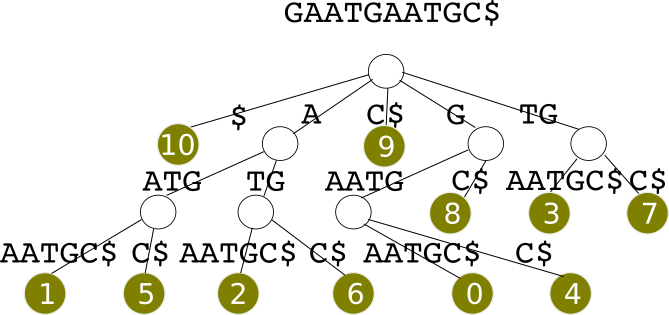
\includegraphics[width=0.8\textwidth]{images/suffixtree.png}
    \caption[Suffix Tree of String GAATGAATGC]{Suffix Tree of the text $T$ = \texttt{GAATGAATGC}. There do exist tools, that show the creation of such trees for educational purpose\footnote{\url{https://visualgo.net/suffixtree}}.}
\end{figure}
As can be seen in this example, the information can be redundant, so that improvements in the form of suffix array and FM-Index are used in computational biology. The suffix array is a ordered list of all suffixes, that can be directly be used for the FM-Index, based on the Burrows-Wheeler Transformation. This is used in most common mapping tools for DNA/RNA-read mapping, the most prominent being BWA \cite{Li2013a,Li2009} and Bowtie \cite{Langmead2009, Langmead2012}. While a suffix tree would need approx. 45GB of memory for the whole human genome DNA, the Suffix Array requires 12GB, and the FM-Index only about $\sim$ 1GB of memory \footnote{\url{https://www.coursera.org/learn/dna-sequencing/lecture/r8Xh3/lecture-genome-indexes-used-in-research}}
\begin{figure}[!ht]
\label{fig:k-mer}
    \centering
    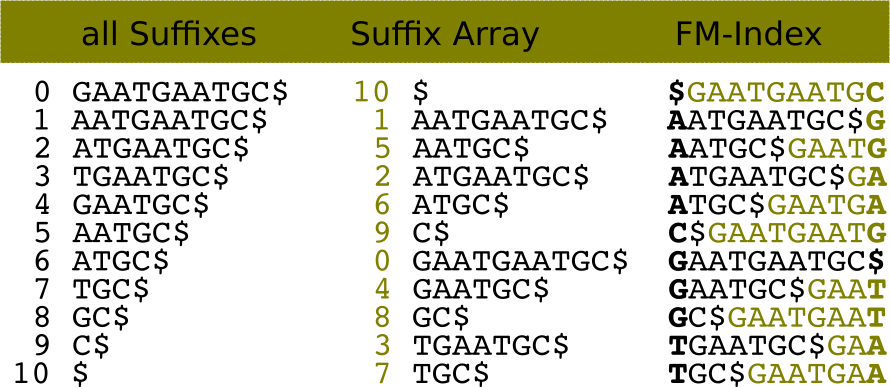
\includegraphics[width=1\textwidth]{images/suffix.png}
    \caption[Construction of suffix array]{Construction of suffix array, based on all suffixes, and ordered lexicographically ascending. The FM-Index extends the entries in the suffix array, by calculating the Burrows-Wheeler Transformation \texttt{CGGAAG\$TTAA}}.
\end{figure}
\end{itemize}
\subsection{Inexact String Matching}
DNA reads from modern devices, show much higher error rates, compared to Sanger based Sequencing. Third generation sequencing devices like MinION from Oxford NanoPore Technologies\footnote{\url{https://nanoporetech.com/products/minion}} showed a per base error with Phred-Score 7 (error rate $sim$ 15\%) with the initial chemistry R7. Even with the latest chemistry R9.4 used in the whole genome sequencing project of NA12878\footnote{\url{https://github.com/nanopore-wgs-consortium/NA12878}}, the error rate is about 10\% per base. Using exact string matching is not only limited by these errors, but also by the variation. The previously described Levenshtein distance or edit distance problem can be solved with  dynamic programming.      
\label{inexact}
\subsubsection{Dynamic Programming}
For solving the pairwise alignment problem, two different approaches are available, based on some similar underlying assumptions, solving however different problems. Both approaches rely on substitution scores, and are in  $\mathcal{O}({n m})$ for length $n$ and $m$ of two strings $S_1$ and $S_2$. The global or often referred to as Needlman-Wunsch alignment tries to align sequence pairs, so that all letters from both sequences are taken into consideration. The local alignment differs in this regard, by considering alignments, where the costs of a substring of either $S_1$ or $S_2$ can be improved compared to the global alignment. Both approaches are build by a matrix with of size (n $\times $ m).
\subsubsection{Global Alignment}
The global alignment, addressed by Needleman-Wunsch \cite{Needleman1970}, contains all nucleotides from both sequences $S_1$ and $S_2$. A simple form of the substitution costs are 1 for match, 0 for mismatch and -1 for indels (gaps). Sequence $S_1$ and $S_2$ are used for column and rows in the matrix that will be used for dynamic programming. Figure \ref{fig_global} represents the two steps: filling in the score table, and walk back in the traceback table. For filling in the score table, the match/mismatch and gap scores are required. There are different predefined substitution matrices, like PAM250\footnote{\url{http://www.mbio.ncsu.edu/bioedit/tables/PAM250}} or BOSUM62\footnote{\url{https://www.ncbi.nlm.nih.gov/Class/FieldGuide/BLOSUM62.txt}}, widely used for amino acid changes. For the sake of simplicity, the score table is used 
as following:
\begin{figure}[H]
\label{fig:global}
    \centering
    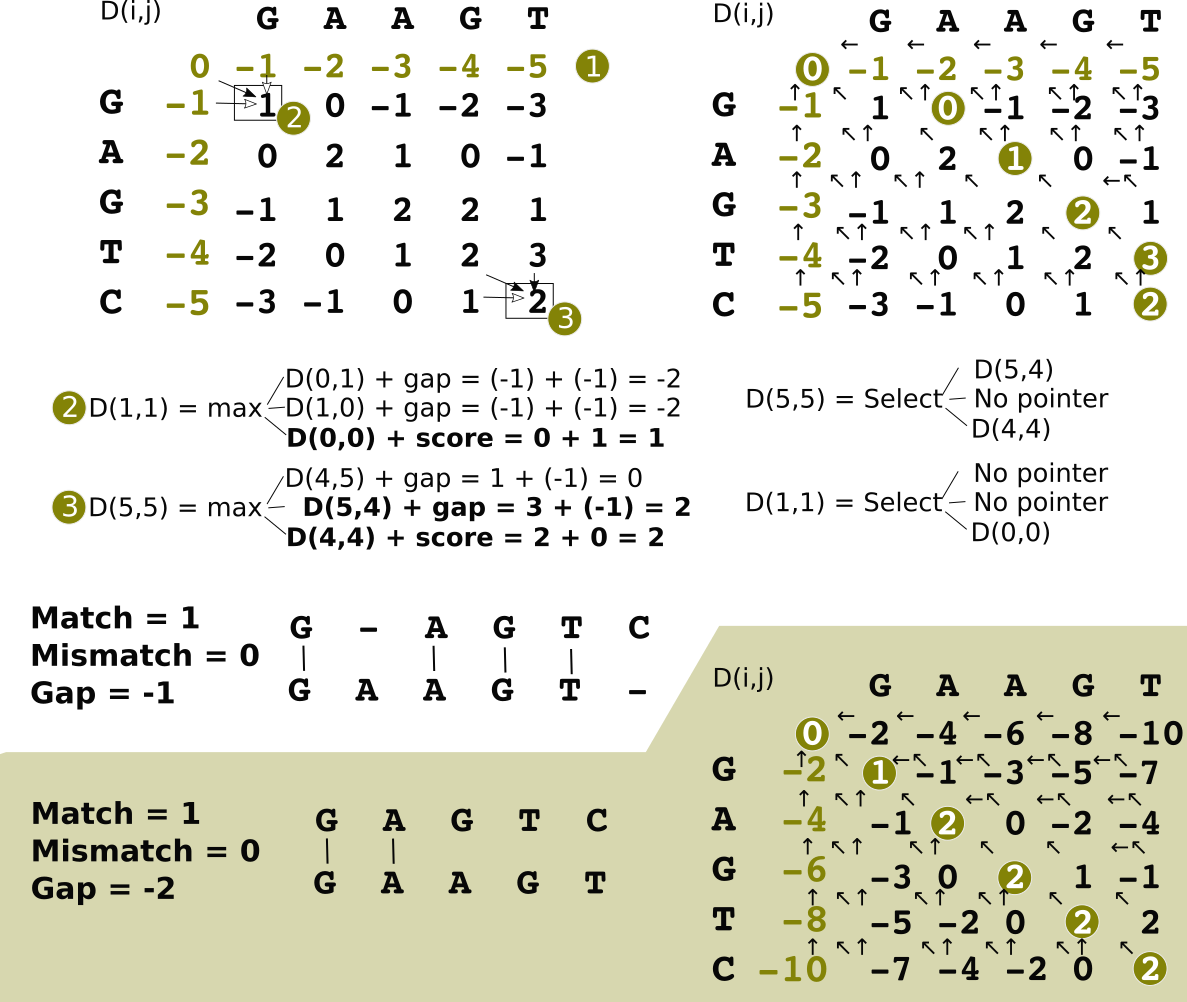
\includegraphics[width=1\textwidth]{images/globalAlign.png}
    \caption[Example of Global Alignment]{Example of Global Alignment, with 2 different gap scores (gap -1 and gap -2 (light-olive background)). The gap penalty and matching scores influence the alignment significantly, with two different results: 4 matches, 1 insertion and 1 deletion versus 2 matches and 3 mismatches.}
\end{figure}
\begin{table}[H]
\centering
\caption{Score Table, indicating the score for a match (1) and mismatch (0)}
\label{scoreTable}
\begin{tabular}{lllll}
  & \texttt{A} & \texttt{C} & \texttt{G} & \texttt{T} \\
 \texttt{A} & \cellcolor[HTML]{808000}1 &   &   &   \\
\texttt{C} & 0 & \cellcolor[HTML]{808000}1 &   &   \\
\texttt{G} & 0 & 0 & \cellcolor[HTML]{808000}1 &   \\
\texttt{T} & 0 & 0 & 0 & \cellcolor[HTML]{808000}1
\end{tabular}
\end{table}
In a first step, the gap penalty score is added in the first row, and first column, by summing up with the previous value (Figure 1, (1)). Subsequently the table is filled by recursively iterating over all entries in the matrix, and calculating the maximum value for the current cell $D_{i,j}$:
$ D_{i,j} = \max
  \begin{cases}
    D(i-1,j)+ \text{gap penalty}      \\
    D(i,j-1)+ \text{gap penalty} \\
    D(i-1,j-1)+ \text{matching score} \\
  \end{cases}
$


\subsubsection{Local Alignment} \label{localAl}
The Smith-Waterman algorithm \cite{Smith1981} as \textit{the} representation of a local alignment, is based on dynamic programming for finding substrings / regions of highly similar content. Since all possible alignments are considered, the optimal local alignment is guaranteed to be found. In the first step, the first column and first row are set to 0 instead to the gap-penalty score. Further a $0$ is added in the cases, so that negative entries are not possible. 
$ D_{i,j} = \max
  \begin{cases}
    D(i-1,j)+ \text{gap penalty}      \\
    D(i,j-1)+ \text{gap penalty} \\
    D(i-1,j-1)+ \text{matching score} \\
    0 \\
  \end{cases}
$\\
The filling of the scoring table is again a recursive step like in the global alignment. The traceback does not start in the cell D(n,m), but in the cell with the highest value. Figure \ref{fig:local} represents the same examples as for local alignment. Here the starting point for the traceback is however the highest entry in the scoring table. The end is reached by finding the cell with a value 0. This is very different from the global alignment, that always starts in cell $D(n,m)$ and ends in cell $D(0,0)$. Optimisations of this approach are presented in Gotoh \cite{Gotoh1982}.  
\begin{figure}[H]
\label{fig:local}
    \centering
    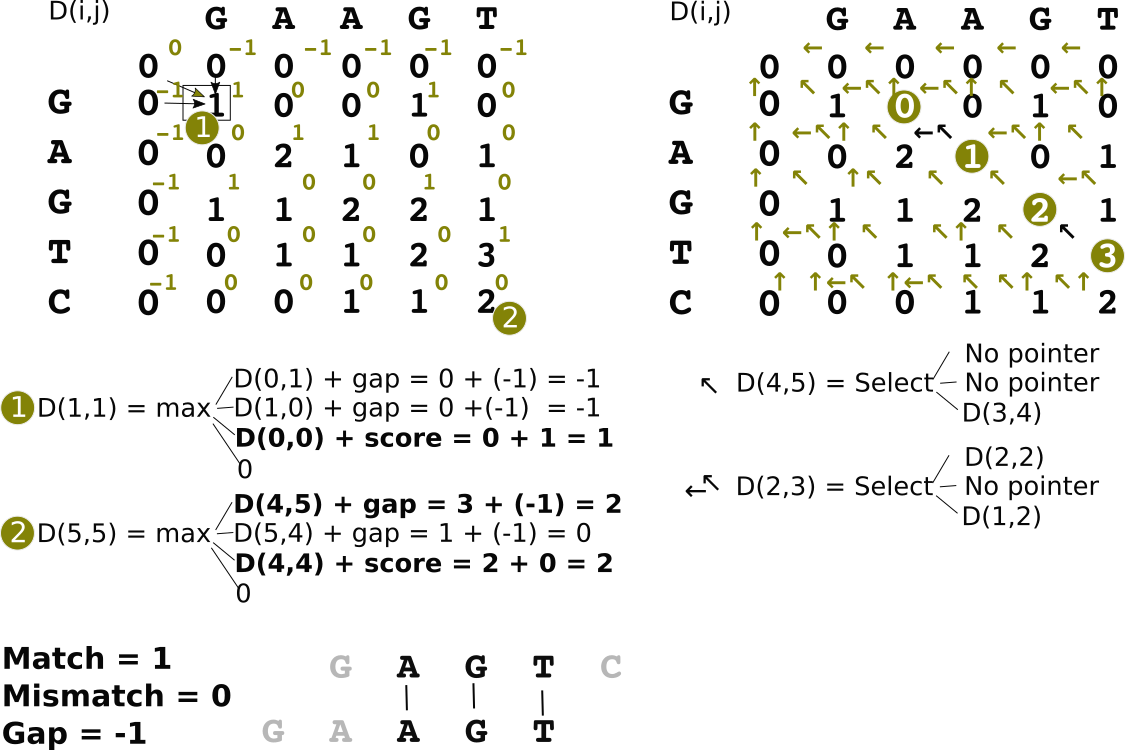
\includegraphics[width=1\textwidth]{images/localAlign.png}
    \caption[Example of local alignment]{Example of local alignment, with the Match/Mismatch/Gap scores as previously defined. As can be seen, only the part with the highest similarity \texttt{AGT} as substring of text $S_1$ and $S_2$ is the best result for the local alignment}
\end{figure}
%\subsection{Biological Networks}
\section{Aligning mtDNA sequences}
Although there exists plenty of alignment software performing pairwise alignment\footnote{see extensive list of pairwise sequence alignment tools here \url{https://omictools.com/pairwise-sequence-alignment-category}}, based on the previously described algorithms, the alignment for mitochondrial genomes comes with special requirements. Algorithms developed for the alignment of nuclear DNA often have issues with the correct nomenclature used for mitochondrial DNA. Also the circular structure of the mtDNA, where a start does not necessarily have to be at position 1 when linearized, needs further attention. 
\subsection{Related Work}
While there do exist approaches specifically for mtDNA, the available tools currently slow run-times and are not feasible for processing 1,000s of mtDNA sequences in feasible time. The overview of those tools is much clearer:
\begin{itemize}
\item \textit{MitoTool} accepts fasta files from either D-Loop (position 16024-574), the complete mtDNA sequences or to analyze mtDNA genome sequences lacking the D-loop region. However no information is provided about the algorithm used \cite{Fan2011,Fan2013}.
\item \textit{Phy-mer} \cite{Navarro-gomez2014} accepts full mtDNA sequences, and does not generate variant files, but rather performs a haplogroup comparison based on this k-mer, and alignment-free approach. Phy-mer is available on GitHub\footnote{\url{https://github.com/MEEIBioinformaticsCenter/phy-mer}}, providing  the older Phylotree 16 version.
\item \textit{MUMmer} is a suffix-tree based approach already described in 1999 \cite{Delcher1999} and updated to version 3.0 in 2004 \cite{Kurtz2004}. Currently version 4.0 is in preparation, updated to support multithreading and genomes of any size\footnote{\url{http://mummer.sourceforge.net/}}. Altough not explicitly designed for mtDNA, we will compare Mummer 3.0, since being integrated in HaploFind (see Chapter \ref{hg:related}
\item \textit{mtDNAprofiler} \cite{Yang2013} is accessible via web\footnote{\url{http://mtprofiler.yonsei.ac.kr/}}. It implements two main rules, the first to use the least number of differences to the rCRS, and the second considering realignment of indels in the mtDNA like AC repeat, HV2 C-stretch and 
\item Even professional alignment Software such as Sequencher[ref Sequencher] fail in aligning mtDNA sequences correctly, requiring a experienced user to correct the contigs consensus. 
\item \textit{MitoTyper}: Several rules have been defined to overcome the special problems in the alignment of the mtDNA to the revised Cambridge Reference Sequence (rCRS)[Anderson S, Andrews RM]. The first rules were designed by Wilson et al. \cite{Wilson2003} in the alignment an nomenclature protocol, the so called “Wilson rules”. These rules were generally accepted, but often led to ambiguous naming of the sequences. Budowle et al. \cite{Budowle2010} extended these rules for the human mitochondrial DNA control region. The reliability was shown on the Scientific Working Group of DNA Analysis Methods (SWGDAM) database\footnote{\url{https://www.swgdam.org/}}.Unfortunately we were not able to test either the commercial software nor to access the SWGDAM database. 
\end{itemize}
Furthermore the comparison of rule-based alignment versus phylogenetic based alignment has been debated in the scientific community [Bandelt, Parson – Consistent treatment of length variants in the human mtDNA cR][Deborah Polanskey – Comparison of mitotyper…]. Both approaches come to the conclusion that novel polymorphisms may require additional rules and that ambiguity in mtDNA alignment can never be excluded. We are aware of both approaches and combine rules with phylogenetic nomenclature based on currently available data.
%\subsubsection{Pairwise alignment}
%\subsubsection{Multiple sequence alignment}
\subsection{Sliding Window Smith Waterman approach}
Given the small size of mtDNA with its $\sim$ 16,569 basepairs, constructing a matrix $D(n \times m)$ corresponds 274,5311,761 cells that need to be calculated for 2 sequences with length $(n,m) = 16,569$. This means that for comparing 2 sequences we need 274.5 million steps for calculating the alignment. By splitting sequences in chunks with length of 200 base pairs and using an sliding window approach to overlap these pieces to avoid losing differences to the rCRS between the chunks. This way we get 82 chunks, each with 220 bases (20 overlapping bases, since longest known insertion currently in Phylotree is 8289.1CCCCCTCTACCCCCTCTA with 18 bases), yielding to $82 x 220^2 = 3,9$ million steps resulting in a reduction of calculation time from 41,7 seconds to ~0,6 seconds per sample performed on an Intel Core i3 with 3GB main memory. This is a 69-fold reduction of calculation time. \\

Further advantage of current multicore CPU architectures is taken, allowing parallel calculations on the different cores. We achieve this by using Java’s Thread Pool methods and work queues, being aware of pool-related deadlocks, resource thrashing and thread leakage. [Identifying Performance Deviations in Thread Pools]. On a Dual Core Processor we gain 30\% of speedup, on a Quad Core Processor we get a calculation time of ~ 200 milliseconds equal to a speed up of factor 3.
\begin{figure}[!ht]
\label{fig:local}
    \centering
    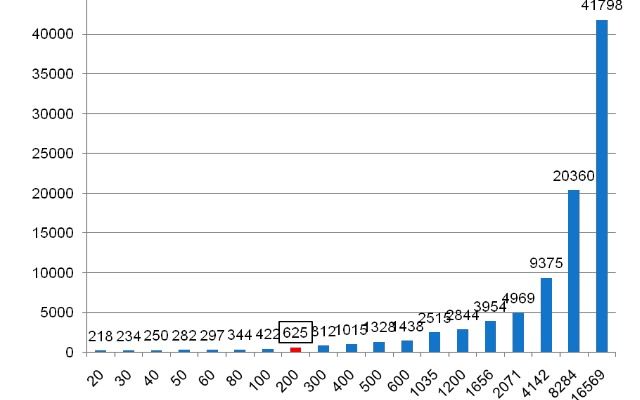
\includegraphics[width=1\textwidth]{images/runtimeSW.png}
    \caption[Runtime in ms of Gotoh for n/i ]{Runtime in ms of the local alignment, considering all basepairs n. If the mtDNA is chopped in 84 pieces of length 200, the calculation takes 625ms instead of 41,798 ms when unchopped}. 
\end{figure}
While this basic approach outperforms various tools in the runtime, it is still too slow to align large set of sequences with several thousand sequences. 
\subsection{K-mer Hash table based approach}
Given the highly similarity of mtDNA sequences, the use of k-mer based approaches for identifying identical reads where the cost-expensive dynamic programming (either global or local alignment) can skip those costly alignments. 
\subsection{Optimizations}\label{align:optim}
\section{Comparison to Data Structures}
Validation of alignment accuracy
We based our first tests on 5300 fasta sequences out of 7843 (since not all sequences were complete, not available in Genbank or not existent as haplotypes) and their assigned haplotypes files from the Phylotree Website available until February 2011. By using parametrized test cases with Junit [http://www.junit.org/] in the Eclipse software development environment [www.eclipse.org/] the comparison of aligned sequences to the haplotypes files was straight forward. We noticed soon that in the most cases the results were as expected. For this first test it was sufficient to set the gap penalties of Smith Waterman so that the selected alignment with the least number of differences between the sample and the rCRS sequence is established. This corresponds to Rule 1 – Least number of Differences defined by Budowle et al. [ref budowle – automated alignmentand nomentclature]. We further adapted Rule 2 – Maintain the AC Repeat Motif , as well as Rule 3 – Prefer Substitutions to Indels. We also had to take care of the position where an insertion or deletion is performed by SW, since the direction was 5’ to 3’ instead of 3’ to 5’. Therefore we implemented a rule shifting such position to the rightmost occurance of the same base, e.g. SW detects a deletion on 15940T, but since the bases in the rCRS from 15940 to 15944 are all thymine, the correct position is 15944d. To guarantee that the sequences used in HaploGrep can be assigned the correct haplogroup, we downloaded all sequences from NHI Genbank  to take all sequences used for Comparison with alternative Software Solutions
\subsection{Suffix Trees}
\subsection{Suffix Array}
\subsection{FM-Index}
\subsection{Result}
\section{Conclusion and Outlook}
Several well established approaches to align nucleotide sequences with numerous algorithms facing this problem[blast(ncbi blast, psi-blast), fasta(fasta, ssearch, fastm, ggsearch), Hidden Markov Models (hmmer, sam) ] do exist. However only a few sequence alignment tools for mitochondrial DNA do exist, performing either poor regarding calculation time or nonsatisfying in the context of reliable alignment due to the special characteristics of mtDNA structure. Although there are several guidelines on how to align mtDNA data [Wilson Rules, SWGDAM-rules], expertise knowledge is still needed. We therefore designed a new sequence alignment tool for the fast and reliable alignment of full mitochondrial DNA sequence data. As a result we extend our mitochondrial workbench HaploGrep 2 with the herein described alignment module to allow an accurate and easy handling of mtDNA Fasta files.
%De-novo vs. mapping assembly Wikipedia Artikel!! 
%Paper: A Practical Comparison of De Novo Genome Assembly Software Tools for Next-Generation Sequencing Technologies





\cleardoublepage
\chapter{MapReduce for mtDNA High Throughput Sequencing: mtDNA-Server}
\label{chap:NGS}

The first decoding of the full genome by the Human Genome Project was finished after 13 years (earlier as expected) in 2003 \cite{InternationalHumanGenomeSequencingConsortium2004}. Since then, not only the sequencing methods but also the algorithms for data processing improved constantly. Further the prices dropped from US\$3 billion to the long awaited \$1000 for sequencing a whole human genome (3.2 billion base pairs)\footnote{http://blogs.nature.com/naturejobs/2015/10/08/big-data-the-impact-of-the-human-genome-project/} generated within just hours/days. Therefore, the bottleneck shifted from data generation to data processing. This is the result of the so called second generation or next-generation sequencing devices, which deploy a massively parallelization sequencing. Thereby millions of short reads are read out, and the data processing wouldn't be possible without the improved Bioinformatics and computer science based tools. 

To process this \textit{"data-flood"}, soon parallel computing architectures are required. Even though only about 1 percent of the complete genome is derived from the mitochondria, the higher content compared to the nuclear genome results in an increased file size. 

This Chapter presents a system called mtDNA-Server \cite{Weissensteiner2016b}. It was designed as Software as a Service, to process next-generation sequencing reads of mitochondrial DNA, independently of the sequencing strategy. Target mtDNA sequencing, whole genome sequencing (WGS) or whole exome sequencing (WES) data can be analyzed. Since mitochondria play an important role in cancer \cite{Brandon2006,He2010,Guo2012,KlossBrandstatter2010}, with this new high-coverage data, also deeper understanding in the development or progression of cancer can be provided. The debate whether mutations help drive the tumor, or are bystander events can now be explored with this new sequencing method \cite{McMahon2014,Kloss-Brandstatter2015}. Further scientific relevant questions are the influence of the mitochondrial genome in the process of aging or in other disease such as neurodegenerative diseases. Here, mtDNA-Server can help the researchers by hiding the complexity of the data processing and providing additional quality control, to avoid the publication of false positive results. 

\section{Background: Parallelism is the Key}
When Google described it's framework MapReduce in 2004 \cite{Dean2008}, the NGS devices began their triumphal procession of massively parallel sequencing (MPS). While the NGS devices produced parallel data of genomic sequences, the parallelism in the MapReduce programming paradigm is achieved by splitting data to key/value pairs which are processed in the Map phase and the Reduce function on huge clusters of commodity hardware. In 2009, first approaches based on MapReduce entered the field of genetics \cite{Schatz2009}. The term Cloud-computing got established shortly thereafter 2010 \cite{Schatz2010}. The same time our group began investigating the potential of MapReduce for Genomics with first results presented in 2011 \cite{DBLP:conf/gvd/SchonherrFWKSK11}. The presented solution in this chapter is based on Apache Hadoop and the execution framework Cloudgene \cite{Schonherr2012} developed by Sebastian Sch\"onherr and Lukas Forer as partial fulfillment of their PhD requirements. Cloudgene allows the straight-forward realization of MapReduced based workflows, based on a YAML\footnote{{http://www.yaml.org/}}-configuration files, thereby automatically generating the graphical user-interface. 

\section{Burrows-Wheeler vs. Hashing}
The alignment and mapping of short reads generated by NGS devices to a reference genome is crucial for identifying variants on the DNA or RNA. Therefore after the quality control of the raw files with tools such as FastQC\footnote{\url{(http://www.bioinformatics.babraham.ac.uk/projects/fastqc/)}}, sequence mapping is required. Various approaches for this task were designed, resulting in dozens of short read mapping tools  \cite{Hatem2013,Pabinger2013}, with different strength and weaknesses. The two most important classes are Hashing (of overlapping k-mer words) and Burrows-Wheeler Transformations. While Hashing is consuming more memory for large reference genomes, it is very fast for exact matches, and therefore best used for highly similar sequences (see Chapter \ref{chapterAlignment}). The reference size is however not an exclusion criteria for the mitochondrial genome with its small size of less than 17kb. This approach is applied in tools like SMALT, SOAP or SSAHA2. Burrows-Wheeler based approaches like BWA \cite{Li2009}, Bowtie \cite{Langmead2009} or SOAP2 are fast and show a high sensitivity, also for repetitive regions, where Hashing shows less sensitivity. The principal concept of Burrows-Wheeler Transformation is to compress an Suffix-Tree. Thereby the index itself can be compressed, by permuting the order of characters representing the nucleobases in such manner, that characters are resorted and ordered according repeats. For the herein presented solution, BWA MEM \cite{Li2013a} was considered to have the best trade-off between speed and accuracy and is largely accepted in the genetics field (e.g. used in the 1000 Genomes Project \cite{Abecasis2012}).

\section{Related Work}
Several tools for sequence alignment/mapping were developed with the increase of data generated by NGS devices. While most of the tools are written in C/C++, Python or Java very few tools came with a user-interface. Also most of those tools are developed for linear DNA, not considering the circular structure of mtDNA. While the alignment/mapping is just the first step for data processing, several other steps are required, to cover the spectrum from alignment to the representation and annotation of the variants. Those steps comprise the following classifications, whereby an extensive overview of the different tools per step can be found in Pabinger et al. \cite{Pabinger2013}. 
\begin{enumerate}\label{enum:NGS}
\item alignment/mapping of the raw reads to the reference genome considering the circular structure
\item sort the generated BAM file and process the mapped reads
\item perform a variant calling considering low level heteroplasmy, by applying specific models
\item classification of variants to haplogroups
\item perform a quality control in order to prevent misinterpretation of contamination 
\item annotate the variants and generate reports
\end{enumerate}

For scientists in the lab, where Linux-environments are often lacking, single tools or the complete pipelines are often not accessible. One initiative to make the creation of workflows/pipelines accessible to scientists in life science, is the \textbf{Galaxy Project} \cite{Goecks2010,Afgan2016}. Galaxy allows the generation of workflows in a graphical way, by providing a large selection of Bioinformatic applications, that can be connected interactively with "point and click". Galaxy got extended by Galaxy CloudMan \cite{Afgan2010}, which allows deploying computing cluster on the Amazon EC2 cloud infrastructure. The Galaxy group also published two workflows presented in \cite{Goto2011} and \cite{Dickins2014} where mitochondrial genomes from NGS devices was processed and the data as well as the pipeline was made freely available. The pipeline comprises 43 steps, that cover all the previously mentioned steps in NGS mtDNA analysis. For mapping BWA is used, the resulting SAM file gets filtered and converted to BAM file, the pileup file gets generated and several filter for forward and reverse reads are applied. A cleaned variant file with heteroplasmic levels that differ above 1\% from the reference base are reported as result.

\textbf{Mitoseek} \cite{Guo2013} was developed for exome and whole genome sequencing data of the mitochondrial genome. Mitoseek is written in Perl and combines several steps. As a first step, the already mapped BAM file gets extract mitochondrial reads that don't map to the nuclear DNA, due to the presence of Numts (nuclear copies of mitochondrial DNA) \cite{Parr2006, Dayama2014}. Basic quality control is performed by generating plots of the per base sequence quality as well as the length distribution of the reads.  Mitoseek also performs the variant calling and allows to detect 0.1 \% of heteroplasmy if the coverage of 10,000x is present. Besides the filters provided by the user, Mitoseek implements statistical frameworks for the assessment of heteroplasmy and also detects somatic mutations, by comparing tumor-benign pairs of samples. It however lacks a graphical user interface and does not allow to check for haplogroups.

One of the first tools with a convenient web-based user-interface for the analysis of mtDNA NGS data was presented in Zidhkov et al. \cite{Zhidkov2011}. \textbf{MitobamAnnotator} starts with the mapped BAM file to the rCRS or the Yoruba Sequence used in HG18 by using Samtools \cite{Li2009} to process the reads. It takes the user input for filtering by three different categories (high quality read parameters, consensus calling parameters and heteroplasmy parameters) and annotates the heteroplasmic variants with the scores and writes files for haplogroup classification in HaploGrep. It is however limited to one file per upload of 500MB. 

\textbf{MtoolBox} is a pipeline for heteroplasmy annotation and prioritization analysis of human mitochondrial variants in high-throughput sequencing \cite{Calabrese2014}. The workflow starts with BAM or FASTQ files and maps the raw reads with GSNAP \cite{Wu2010}. Besides the dependency to GSNAP, MToolBox which is written in Python relies on Samtools and MUSCLE \cite{Edgar2004}. It performs a realignment around known insertions and deletions based on the Genome Analysis Toolkit GATK \cite{McKenna2010} and marks duplicates based on the Picard Tools\footnote{\url{http://broadinstitute.github.io/picard}}. The variants are called by a fragment-classification tool to detect the heteroplasmic fraction (called HF) and the related confidence interval for each position of the mitochondrial genome. As a result a VCF file and the haplogroup assignment as well as the functional annotation (similar to  the information provided in MitImpact \cite{Castellana2014}) are generated. MToolBox is made available with a user-interface on MseqDR\footnote{\url{https://mseqdr.org/mtoolbox.php}} presented in Shen et al. \cite{Shen2015} .  

\textbf{mit-o-matic} defines itself as a comprehensive computational and experimental pipeline for clinical evaluation of mitochondrial variations from next-generation sequencing datasets \cite{Vellarikkal2015}. The pipeline comes with an online user-interface\footnote{\url{http://genome.igib.res.in/mitomatic}}. limited to file uploads of 25MB per sample of FASTQ files. Three mapping tools are directly supported to map the raw reads to the rCRS reference sequence: BWA, BOWTIE and MAQ. Option 2 accepts the parsed pileup file which is generated with the download version of mit-o-matic (available only after applying for a lincense), not limited to the 500x coverage otherwise. The variant calling is a done by calculating the percentages of reads showing the variant allele out of the total. Annotation is based on Mitomap\footnote{\url{http://www.mitomap.org}} presented in Lott et al.\cite{Lott2013} as well as mtDB\footnote{\url{http://www.mtdb.igp.uu.se/}}, MitoLSDB \cite{K2013} and Sift for predicting the functional effect of a heteroplasmic induced amino acid substitution. Haplogroup prediction is based on Mitotool \cite{Fan2011,Fan2013}. 

\textbf{LoFreq} \cite{Wilm2012} is not limited to mitochondrial genomes and is one of many variant caller available. It was however validated with mitochondrial genomes and was designed to detect 0.05\% of variants. It accepts the mapped BAM file and comes without the need of specifying any parameters. The variant calling is superior to the most herein presented related work. It is based on a Bernoulli trial, where success corresponds to the reference base, and failure to the variant base (K). A Poisson-binomial distribution handles each Bernoulli trial with distinct success probabilities and calculates the exact P-values for observing a variant base in a recursive way. Since this approach is $O(N^2)$ run time optimization were applied so that LoFreqs worst-case runtime is $O(KN)$. LoFreq's result is a VCF file, however without the required FORMAT and SAMPLE columns, since LoFreq was not designed for calling genotypes, but rather low-level variants.

Table \ref{comparisonRelatedWork} gives a summary of the herein outlined tools. Comparison to our mtDNA-Server cloud-application is made, with the method described in more detail in this Chapter.

\begin{table}[h]
\centering
\caption{Comparison of related work - the numbers in brackets represent the enumeration of the different steps in \ref{enum:NGS}}
\label{comparisonRelatedWork}
\begin{tabular}{|l|l|l|l|l|l|l|l|}
\hline
Feature & \begin{tabular}[c]{@{}l@{}}Gal\\ axy\end{tabular} & \begin{tabular}[c]{@{}l@{}}Mito\\ Seek\end{tabular} & \begin{tabular}[c]{@{}l@{}}M.Bam\\ Annot.\end{tabular} & \begin{tabular}[c]{@{}l@{}}MTool\\ Box\end{tabular}. & \begin{tabular}[c]{@{}l@{}}mit-o\\ matic\end{tabular} & LoFreq & \begin{tabular}[c]{@{}l@{}}mtDNA\\ Server\end{tabular}\\
\hline
FASTQ (1,2) & + & - & - & + & + & -& + \\
BAM (3) & + & + & + & + & - & +& + \\
Low-level (4) & + & + & + & + & - & +& + \\
Cont.Check(5) & + & - & - & - & - & -& + \\
Reports (6) & + & + & + & + & + & -& + \\
GUI & + & - & + & + & + & -& + \\
Haplogroups & - & - & + & + & + & -& + \\
Parallel & - & - & - & - & - & -& + \\
VCF & + & - & - & + & - & +& - \\
\hline
\end{tabular}
\end{table}
\section{mtDNA-Server: MapReduce for mtDNA NGS Data}
Both areas of research, i.e. MapReduce for computer science and NGS for life sciences are well established. Our approach brings MapReduce to the field of genetics, and represents one of the first real use-case. By taking advantage of the Apache implementation Hadoop \cite{White2009}, our group previously implemented Cloudgene \cite{Schonherr2012}, a middle-layer to automatically generate the user interface. It was previously designed with two modules: Cloudgene-Cluster and Cloudgene-MapRed. While Cloudgene-Cluster was used to instantiate a cluster on a public cloud, like Amazon's EC2, Cloudgene-MapRed represents the layer between Hadoop and the mtDNA-Server application. It comes with its own workflow engine (a Directed Acyclic Graph Manager) and its own workflow definition language and enables to execute different applications on top of it in an independent manner. The Cloudgene API provides the means for the execution and monitoring of MapReduce jobs. It also handles the communication with the Hadoop cluster and provides a web interface for all job-related tasks  \cite{Weissensteiner2016b} (see section \ref{webservice}).
%rewritten from paper

mtDNA-Server represents such an application: it is an mtDNA analysis workflow starting with the raw data in FASTQ or BAM format and performs a variant calling that results in reliable detection of heteroplasmic sites and variants, contamination estimates and numerous QC statistics based on R \cite{R} and the knitr package\footnote{\url{http://yihui.name/knitr/}}. To take advantage of parallelism, mtDNA-Server supports the upload of several samples at once. Thereby each input file is further split into independent chunks (called intra-sample chunking) \cite{Weissensteiner2016b}. For parallelization, as earlier mentioned, the Hadoop MapReduce framework\footnote{\url{http://hadoop.apache.org/}} is used. Within Hadoop, a cluster of nodes, each consisting of several cores, processes the chunks (each chunk consisting of a 64 MB package of sequence reads) in parallel in the map function, which gets an input record and maps it to one or more key/value pairs. Thereafter the data is grouped and collected by the framework in the shuffle step and further analyzed or directly returned to the application in the reduce function, getting a single key and a list of values on which an operation can be performed (in this case: count the different nucleobases per position). The presented application is written in Java and a YAML file defines the workflow. The architecture of mtDNA-Server can be drafted in Figure \ref{fig:mtdna-server-architecture}. All MapReduce steps are highlighted with the bold lines i.e. (1) Read Alignment, Quality Control and (2) Heteroplasmy Detection. The contamination check is calculated on the Namenode, as well as the annotation of heteroplasmic sites. Both steps take advantage of the previously described HaploGrep in Chapter \ref{chap:NGS}, which was made available as console version for integrating it in pipelines. 
\begin{figure}[h]
    \centering
    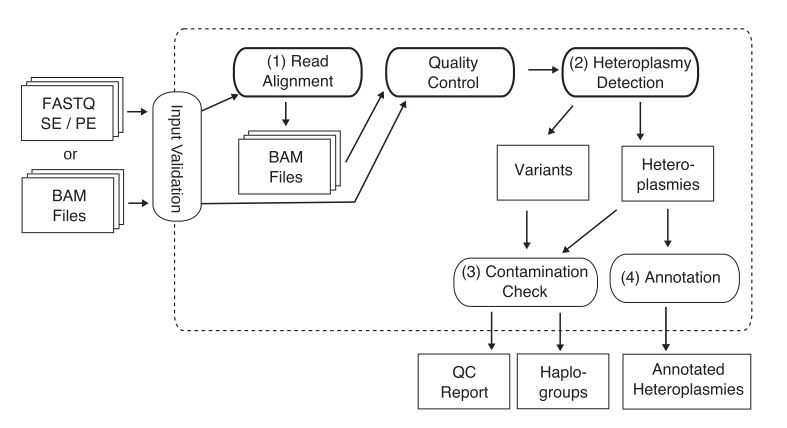
\includegraphics[width=1\textwidth]{images/mtdna-server.JPG}
    \caption[mtDNA-Server workflow for FASTQ and BAM input files]{mtDNA-Server workflow for FASTQ and BAM input files. Figure as represented in \cite{Weissensteiner2016b}}
    \label{fig:mtdna-server-architecture}
\end{figure}
\subsection{Input Validation}
mtDNA-Server allows the upload of FASTQ files, the mapped SAM files or the binary mapped BAM files. The FASTQ files can be paired end or single end, SAM and BAM files are handled with the same input reader. As of May 2017, in total over 45,000 samples were processed - thereby 72\% of all samples were in SAM/BAM format, 12\% in FASTQ single end and 16\% of all uploaded samples were FASTQ paired end files. Depending on the user selected file format, the specific set of workflow steps is executed in parallel. The validation step verifies the selected file format and checks it by automatic format detection of the uploaded files. As a next validation step for the mapped SAM/BAM files, the header needs to contain the mitochondrial reference sequence with length according the rCRS or RSRS, being 16,569. Since the human reference genome until the Genome Reference Consortium Human genome build 37 (GRCh37 or hg19) used an African reference sequence for the mitochondrial genome (Yoruba reference \texttt{NC\_001807.4} with length 16,571. This reference is also accepted, and gets automatically converted to meet the nomenclature of the rCRS (\texttt{NC\_012920.1}). This is crucial for the post-processing steps, especially the generation of the HaploGrep files and the annotation of the amino acid changes. Listing \ref{listBAMheader} represents part of the SAM/BAM header and the required size for chrM = the mitochondrial genome (sometimes referred to as chromosome 26).

\begin{lstlisting}[caption=Header of SAM/BAM file expecting length (LN) 16569 or 16571 for chrM, label=listBAMheader]
@HD VN:1.5 SO:coordinate
@SQ    SN:chr1    LN:249250621
@SQ    SN:chr2    LN:243199373
...
@SQ    SN:chrM    LN:16569
\end{lstlisting}

\subsection{Parallel Read Alignment}
When the Input validation step completes successfully, the input data is put in the Hadoop Distributed File System (HDFS). If the input corresponds to FASTQ files, the raw sequences are mapped to the rCRS reference sequence automatically. This is done with BWA-MEM v 0.7.5 \cite{Li2013a} through the Java bindings (JNI) for bwa version of JBWA\footnote{\url{https://github.com/lindenb/jbwa}} by adapting it to run in the Hadoop environment. FASTQ files can be generated depending on the NGS devices in two different ways: either as paired-end reads (shown in simplified form: a DNA sequence gets read from both sides) or as single-end reads (DNA sequence is read from one side only). Paired-end reads are generally handled in two different files, and the ID of the reads in each file point to the corresponding forward and reverse reads.
The correct read pairs are identified by setting the Hadoop output key to the read name, as previously described \cite{Weissensteiner2016b, Pireddu2011}. Figure \ref{fig:mapreduce} gives an overview of the invoked map and reduce functions. This extra step is not required for single-end reads, were each chunk can be directly mapped with BWA-MEM, and the resulting SAM records are stored in the HDFS. The splitting of the chunks needed adoptions, since the FASTQ file consists of four lines in the file describing one read. After the generation of the SAM file, the BAM files are written, by using the secondary sort mechanism of Hadoop MapReduce. Thereafter, all steps are identical to the direct import of BAM files by the user, described in the next subsection.
\begin{figure}[!ht]
    \centering
    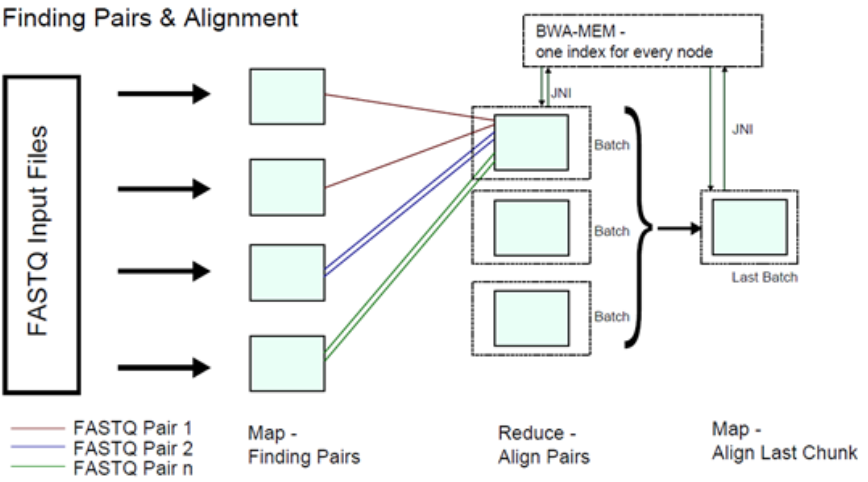
\includegraphics[width=1\textwidth]{images/mapreduce.png}
    \caption[Paired End Read Alignment with MapReduce]{Paired End Read Alignment with MapReduce - The Hadoop map function creates keys consisting of the read ID to sort read pairs. The reducer amounts the read pairs to a batch and executes it via a JNI method (JBWA) with BWA-MEM. Remaining reads are aligned within the Last-Batch method.  }
    \label{fig:mapreduce}
\end{figure}
\subsection{Quality Control}
During this QC step, the BAM input file gets analyzed and basic statistics are generated. This way, the user can get real-time feedback and gets a first idea on how good the data quality of the sequencing run was. These statistics include metrics on how many reads are mapped, how many duplicate reads were filtered or if a reference based issue was found. The example QC report for two samples from the 1000 Genomes project (IDs: HG00096 and HG00740) looks as presented in Figure \ref{fig:mtdna-server-qc}. The high amount of filtered reads indicates a low data quality (below Phred-Score Q20). If a run quits unexpectedly, the FWD Bases and REV Bases would show a significant difference in the amount.  
\begin{figure}[!ht]
    \centering
    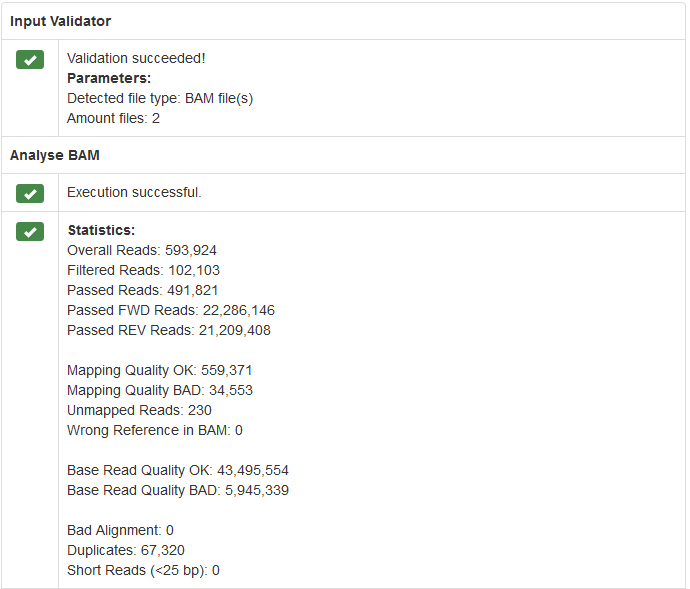
\includegraphics[width=1\textwidth]{images/mtdna-server-qc.png}
    \caption[Example statistics for 2 samples from 1000G]{Example statistics for 2 samples HG00096 and HG00740 from the 1000G data set}
    \label{fig:mtdna-server-qc}
\end{figure}
\subsection{Parallel Processing of BAM File}\label{settings}
When the QC step finishes successfully, the BAM file is processed with Hadoop-Bam \cite{Niemenmaa2012}, which splits the BAM files across the nodes, as previously drafted. Each chunk is processed autonomously and filtered on read (=sequence of n-bases) and base (=the nucleotide A,C,G or T) level. mtDNA-Server filters reads with a mapping quality Phred score Q$<$20  and requires the minimum read length$<$25, as presented in \cite{Zhidkov2011}. Reads being marked as duplicates are also filtered within this step. mtDNA-Server does not search for duplicates on its own, only emits the marked as duplicates reads. Further, mtDNA-Server excludes all reads with an alignment Phred score Q$\leq$30 and applies the per-Base Alignment Quality (BAQ \cite{Li2011}) to all reads by default. BAQ reduces the false variant calls around indels (insertions and deletions) by performing a profile Hidden Markov Model. For this purpose, the GATK \cite{McKenna2010} BAQ implementation has been adapted in order to consider the circular structure of the mitochondrial genome. For each passed read, all bases with a quality Phred score Q $<$20 are also filtered. The remaining passed bases are counted per strand and per site, where the nucleobases are A, C, G, T, N (unknown base) or d (deletion). Each node provides a list of the sums over each bases (\textit{values}) per site (\textit{key}) per chunk.
When the reduce function processes the key/value pairs, in a first step the heteroplasmy rate is calculated and in a second step the homoplasmic (full allele substitution against the reference sequence).
\subsection{Variant Calling}
For the calling of variants, we differentiate heteroplasmic variants from homoplasmic variants. For heteroplasmic variant calling, additional filters and methods are applied: in a first step, mitochondrial hotspots around the polymeric C tracts around site 310 as well as the N on 3107, causing issues with the alignment according to the rCRS are excluded. Sites with coverage $\leq$10 bases per strand are not considered for heteroplasmy detection. For all remaining sites the next filters are:

\begin{enumerate}
\item  a variant allele frequency (VAF) of $\geq$ 1\% for each strand independently  
\item  a variant allele count of three bases per strand 
\item  an Maximum-Likelihood (ML) model according \cite{Ye2014} is applied.The ML model takes sequencing errors per base into account and is applied to each strand \cite{Weissensteiner2016b}. The likelihood function is as follows:
\begin{equation}
  L(f)=\prod_{i=1}^{l} [(1-f) \epsilon_{i} + f(1-\epsilon_i)] \prod_{i=1}^{k} [(1-f) (1- \epsilon_{i}) + f(\epsilon_i)] 
\end{equation}
Where $l$ and $k$ represent the major and minor alleles respectively, $\epsilon$ the sequencing error probability and the parameter of interest is the major allele frequency $f$. 
All sites with a log likeli-hood ratio (LLR) was calculated as 
\begin{equation}
  LRR=\log L({\widehat{f}_{h_1}}) /  L({\widehat{f}_{h_0}}) 
\end{equation}
where $h_0$ represent the model for homoplasmy and $h_1$ the model for heteroplasmy. LLR $\geq5$ are tagged as heteroplasmic sites, which was defined as high-confidence heteroplasmy in \cite{Picardi2012}. 
\item  A strand bias score is applied to check the forward and reverse independently calculated. Since strands are analyzed independently, mtDNA-Server can filter all heteroplasmic sites with a strand bias score $<1$ \cite{Weissensteiner2016b,Guo2012}. The strand bias $SB$ is calculated as follows:
\begin{equation}\label{eq:llr}
  SB=\left| \frac{k_1}{l_1+k_1} - \frac{k_2}{l_2+k_2} \right| / \left(\frac{k_1 + k_2}{l_1+l_2+k_1+k_2}\right)
\end{equation}
where $k_1$ and $k_2$ represent the forward($_1$) and reverse($_2$) strand of the minor allele count, and $l_1$ and $l_2$ represent the forward($_1$) and reverse($_2$) strand of the major allele count. We ignored the presence of a third allele, which is likely the result of sequence or alignment errors.
\item Furthermore we calculate the binomial proportion confidence interval, depending on the coverage of the alleles: the Wilson Score Interval and the Agresti-Coull Interval as proposed in \cite{Calabrese2014}. 
Both are improvements of the normal approximation method of the binomial confidence interval:
\begin{equation}
\begin{split}
  BCI_{upper} = p + \left(z_{1- \frac{\alpha}{2}} \right)\sqrt[]{\frac{p (1-p)}{n} } \\ 
  BCI_{lower} = p - \left(z_{1- \frac{\alpha}{2}} \right)\sqrt[]{\frac{p (1-p)}{n} } 
\end{split}
\end{equation}
where $p$ is the heteroplasmy level of interest (minor alleles / all base counts), $n$ the base count of all bases on a specific site, and  $z_{1- \frac{\alpha}{2}}$ = $1.96$ for a $95\%$ confidence (which assumes an error level of 5\%) or 2.57 for 99\% confidence.
\item The heteroplasmy level (HET.LEVEL) is the calculated as the weighted mean of the minor variant alleles on the forward and reverse strand. 
\end{enumerate}
The files created for download are the unfiltered pileup format file, the annotated files for variants and the HaploGrep input files. Those are generated automatically and made available for sharing or direct download to the user.
\subsection{Contamination Check}
Mitochondrial genomes can be classified into haplogroups, as reported in Chapter \ref{chapterHaplogrep}. The concept that is applied here is that sample contamination can be seen based on a mixture of haplogroups manifesting as low-level heteroplasmy on the haplogroup defining variants, which is covered in more detail in the next Chapter \ref{chapterContamination}. 
\subsection{Annotation}\label{subs:annotation}
We tag positions in low complexity regions (LCR) \cite{Zhidkov2011} and known polymorphic nuclear mitochondrial insertions (NumtS) \cite{Dayama2014}. LCR tagging is particular necessary for Ion Torrent and Roche generated samples, showing an increased per-base error in homopolymeric stretches $geq$4 bases.  The annotation contains: the Map-Locus of the variant, the phylogenetic weight according Phylotree \cite{VanOven2009} as well as the Amino Acid Change, the MutPred-Score \cite{Li-mutpred2009} and the SelectionScore \cite{Pereira2011}.
\subsection{Web Service}
\label{webservice}
As previously mentioned, mtDNA-Server takes advantage of Cloudgene as the underlying platform to build a scalable web service including the automatically generated graphical user interface. mtDNA-Server has been integrated by using Cloudgene’s workflow definition language based in a YAML file and its plugin interface \cite{Schonherr2012, Weissensteiner2016b}. By integrating mtDNA-server as Cloudgene pipeline, it profits from features like user login, real-time feedback as well as data security. Moreover, it enables mtDNA-Server to assemble all possible heteroplasmic and homoplasmic sites, QC statistics, and various plots describing the data as well as contamination detection into an interactive graphical report that can be viewed directly in the web browser or can be shared with collaborators  \cite{Weissensteiner2016b}.
\section{Results}
\subsection{Data Import}
%The two major issues when we tried to publish mtDNA-Server in a first instance, were comments from the reviewers, concerning (i) file upload limitations and (ii) data sensitivity/privacy concerns. To address those issues, we added additional features to mtDNA-Server. 
mtDNA-Server accepts files from different input sources, with the typical file size as represented in Table \ref{mtDNAsource}: 
\begin{enumerate}[label=(\alph*)]
\item   local file upload via web: When using the file upload, data is imported from the users file system to the mtDNA-Server. One or several files can be selected and imported at once. The current upload limit is 5 GB. The limitation here is also the browser, allowing either 2GB upload (the case for Firefox but also more than 4GBs with Google Chrome). 
\item   local file upload via command line tool: mtDNA-Server supports users with high upload demands by providing a command line upload tool which can be downloaded from the mtDNA-Server website\footnote{\url{http://mtdna-server.uibk.ac.at/start.html}}. The upload tool automatically extracts all reads mapping to the mitochondrial genome, so that for some scenarios, only a small portion of the BAM file needs to be uploaded. The QC quality checks are performed locally and mtDNA-Server starts automatically when all checks are fulfilled. For this import, an index file (.BAI) is required for the BAM files. 
\item   import from SFTP Servers or HTTPS Web-Servers: A convenient way to upload data is by specifying a SSH server location. This can be achieved by selecting "Secure File Transfer Protocol" in the Run Screen of mtDNA-Server. The username and the password for the accessing Server are required. A URL consists of the server address followed by the full Unix path. Several paths can be specified in consecutive lines.
\item   import from FTP servers or HTTP Web-Servers: mtDNA-Server can directly work with public available data via HTTP or FTP. This is achieved by opening "URLS (HTTP)" in the dropdown menu and adding the file URLs in the text-area. The direct file-importer extracts only the mitochondrial part of a whole genome /exome BAM file specifies, in an automatic manner. 
\end{enumerate}

\begin{table}[h]
\centering
\caption{Data size and possible sources for mtDNA-Server for processing mitochondrial massive parallel sequencing data \cite{Weissensteiner2016b}}
\label{mtDNAsource}
\begin{tabular}{llll}
\hline
mtDNA data source &  Mean Coverage & BAM file size & run time\\
\hline
Ancient DNA & $\leq$ 100-fold&  $<$10 MB  & $<$ 1 min.\\
Whole exome sequencing &$\leq$ 1,000-fold&  $<$20 MB  & $<$ 1 min.\\
Whole genome low coverage & $\leq$ 3,000-fold & 1-80 MB  & 1 min.\\
Whole genome high coverage & $\leq$ 20,000-fold & approx. 200MB & 3 min. \\
Targeted mtDNA sequencing &$\sim$50,000-fold & up to 1 GB  & 7 min.
\end{tabular}
\end{table}
%Direct file uploads are especially convenient for small sample sizes ($<$100 MB)  \cite{Weissensteiner2016b}. For large samples sizes, mtDNA-Server provides the import tool as well as the web importer from sftp / https or ftp / http to upload large datasets, often already present on Servers. 
To address concerns regarding data privacy and sensitivity, we implemented a wide array of security measures: the HTTPS protocol is used for securing the complete communication with the server. The uploaded input data is deleted  by the system itself as soon as a job terminates. The resulting files are available on the server for a limited period of 7 days. Thereafter all data are erased automatically. The data can also be deleted immediately by the user after downloading or inspecting the results online. Results derived from the public mode are protected by encrypted token URLs only accessible by the user itself \cite{Weissensteiner2016b}.

\subsection{Results and Data Export}
The results generated by mtDNA-Server can be accessed in an interactive report summarizing all findings. Further all the underlying data are provided for download. The HTML report generated in $R$ with $RMarkdown$ based on the $knitr$ package includes all graphical elements directly in this file. The additional files provided for download represent the  heteroplasmic and homoplasmic variants detected by the earlier described settings in \ref{settings}, the HaploGrep input file as well as the related haplogroup classification result file based on Phylotree 16. Further the raw pileup file is made available for download, including base position counts per sample and per site by reporting the forward and reverse LLR as presented in equation \ref{eq:llr}. 
%A SMTP can be configured in the Admin panel of mtDNA-Server to notify the user by sending an email, once a job has finished successfully. 
The HTML report itself presents several quality control (QC) measures  \cite{Weissensteiner2016b}: 
\begin{enumerate}[label=\textbf{QC.\arabic*}]
\item An overview of the selected base-quality based on the ratio of mapped to filtered reads, see Figure \ref{fig:mtdna-server-qc}. 
\item A responsive table listing all heteroplasmic variants, which can be searched, filtered or sorted by the user directly in the browser. 
\item A frequency table listing heteroplasmic sites found in more than two samples, which could indicate potential artefacts. 
\item \label{item:boxplot} A boxplot of the minor allele frequences summarizing the heteroplasmy levels per sample, not considering the reference base.
\item \label{item:barplot}A bar plot of the heteroplasmic sites found per sample: samples showing a large number of heteroplasmic could indicate issues while mapping/artefacts or sample mix ups that need to be checked.  
\item \label{item:maplocus}The map-loci of heteroplasmic sites: here the heteroplasmic sites are represented according the occurrence on the different loci over the whole mitochondrial genome with its coding- and non-coding regions.
\item An interactive table of resulting haplogroups with the HaploGrep quality score (see Chapter \ref{chapterHaplogrep}), the coverage information for each sample, based on the mean forward and reverse coverage over the whole genome, as well as the coverage of the least covered position and the coverage over the whole genome in absolute numbers, which can help especially for ancient mtDNA or mtDNA data derived from exome sequencing, where the mtDNA often is not covered on every site. 
\item  A contamination table indicating potential sample mix-ups, detected on phylogenetic issues, based on 5,437 haplogroups present in Phylotree. 
\item  Coverage-plots for each sample, that highlights issues in targeted re-sequencing studies. Incorrect concentrations of the PCR products results as shifts in the coverage of the used fragments (see Figure \ref{item:coverageplot}). 
\item  An interactive table for homoplasmic sites. For each variant the haplogroup defining status is represented in form of (yes, no and hotspot mutation (the latter does not have any impact on the haplogroup classification) and yield information regarding amino acid changes, phylogenetic weights as presented in HaploGrep 2 and pathogenicity scores and the pathogenicity scores as described in Section \ref{subs:annotation}. Figure \ref{fig:mtdna-server-plots} includes four plots from the final HTML report \cite{Weissensteiner2016b}.
\end{enumerate}
\begin{figure}[!ht]
    \centering
    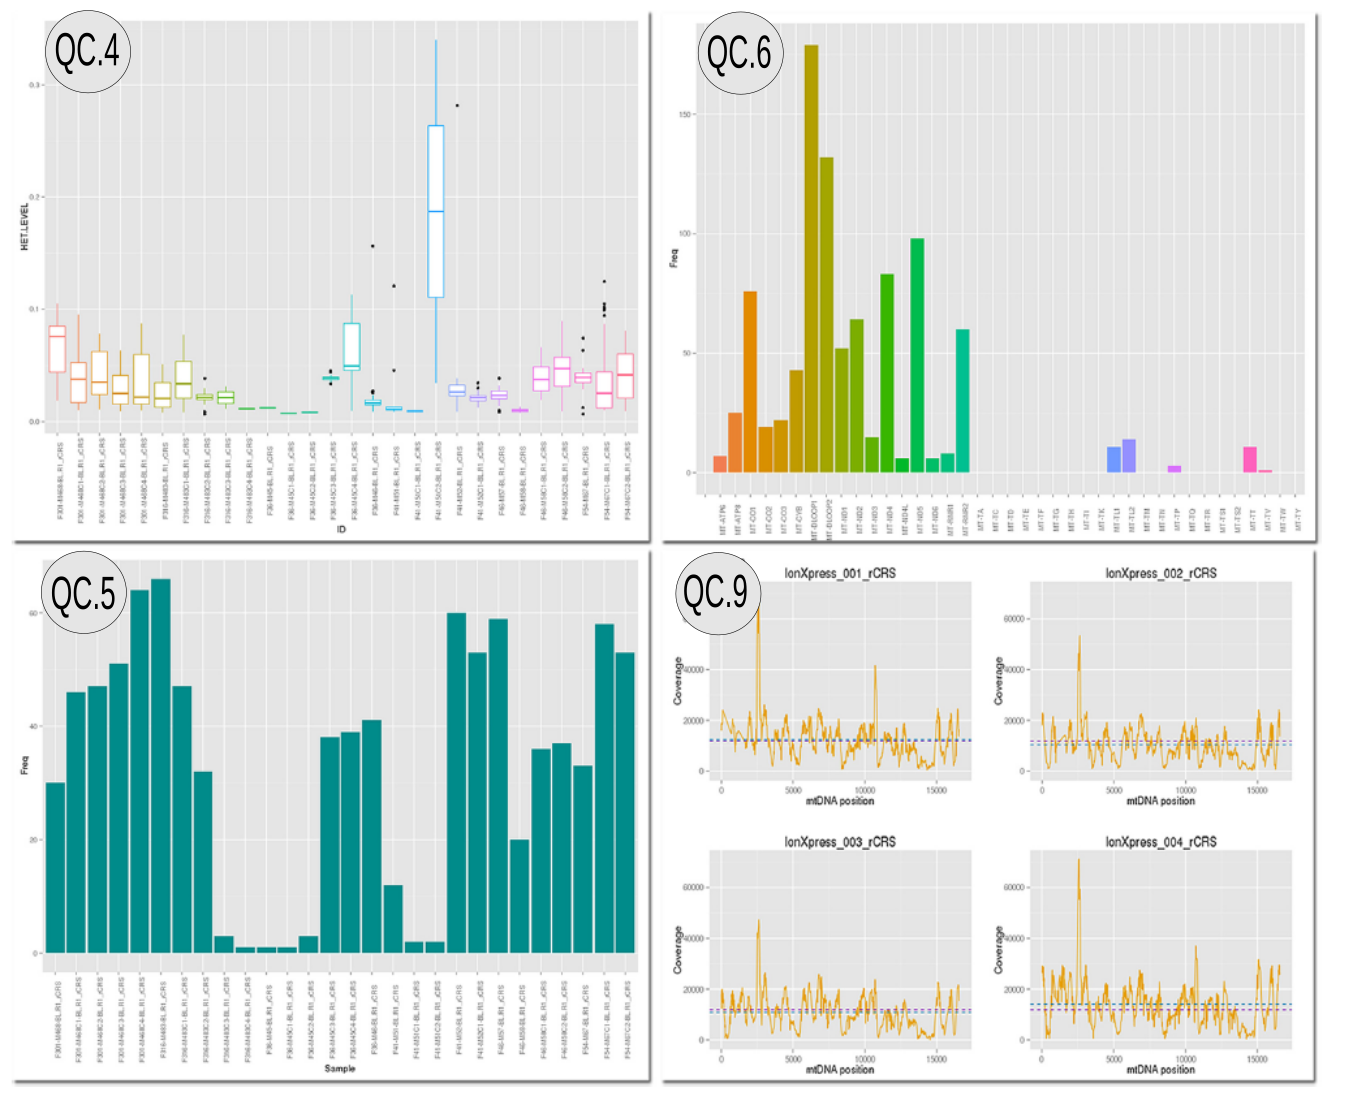
\includegraphics[width=1\textwidth]{images/mtdna-server-plots.png}
    \caption[Plots of the final HTML report]{Four plots of the final HTML report: Boxplot as described in \ref{item:boxplot}, frequency of the minor variant allele independent of reference as a bar plot \ref{item:barplot}, the map locus of the heteroplasmic variants (homoplasmy not considered) on the mitochondrial genome over all analyzed samples \ref{item:maplocus} and the coverage plots for per each sample, indicating the mean coverage over all samples and the mean coverage over all bases \label{item:coverageplot}.}
    \label{fig:mtdna-server-plots}
\end{figure}
\subsection{Validation}
In order to validate our herein presented heteroplasmy detection pipeline, we performed several validation steps and generated data in the lab, based on two blood samples. The concept was presented in our validation study \cite{Kloss-Brandstatter2015}, were we analyzed 28 samples of benign and cancer tissues from oral squamous cell carcinoma on both Sanger as well as Illumina HiSeq 2500 NGS devices. We also applied the mtDNA-Server pipeline within this publication for generating the results. To validate mtDNA-Server we generated 4 different sample-mix ups on the Illumina HiSeq 2500, and on the IonTorrent
PGM, which are also publishe in \cite{Weissensteiner2016b,Kloss-Brandstatter2015}. We run the same samples also on the SOLiD 5500xl, the Ion Torrent Proton, the Illumina MiSeq (with different chemistry) as well as one mix-up on the Oxford Nanopore MinION with the R7 chemistry. The results of the latter devices are part of a publication currently in progress and not reported within this work. The two samples got mixed in the laboratory as follows, by generating artificial contaminations: 
\begin{itemize}
\item Mix1 – 1:2 (50\%) 
\item Mix2 – 1:10 (10\%) 
\item Mix3 – 1:50 (2\%) 
\item Mix4 – 1:100 (1\%)
\end{itemize}
The two Samples were analzed in a prior study \cite{KlossBrandstatter2010}, and the sequences were deposited in GenBank with the following accession numbers:
\begin{enumerate}
\item Sample: HM625679.1\footnote{\url{http://www.ncbi.nlm.nih.gov/nuccore/301505851}} - Homo sapiens isolate Lab002 mitochondrion, complete genome  belonging to haplogroup U5a2e
\item Sample: KC286589.1\footnote{\url{http://www.ncbi.nlm.nih.gov/nuccore/445067603}} - Homo sapiens isolate Lab011 mitochondrion, complete genome  belonging to haplogroup H1c6
\end{enumerate}
We also had the runs of the un-mixed samples Lab002 and Lab011 and could detect low level of heteroplasmic variants that were excluded from the validation (i.e. in Sample Lab002 the heteroplasmic variants on position  15372 and in the Sample Lab011 the sites 7076, 9462, 11150, 15236 and 16129, found as private heteroplasmic mutations in the 1-3\% level). The 27 expected sites that differentiate the two profiles are on position 73, 151, 152, 477, 2706, 3010, 3197, 3768, 5979, 7028, 9145, 9477, 11467, 11719,
12308, 12372, 13617, 14766, 14793, 15289, 16189, 16234, 16256, 16270, 16311, 16362 and 16526 according the rCRS reference sequence, see Figure \ref{fig:mtdna-mix-ups}. 

\begin{figure}[!ht]
    \centering
    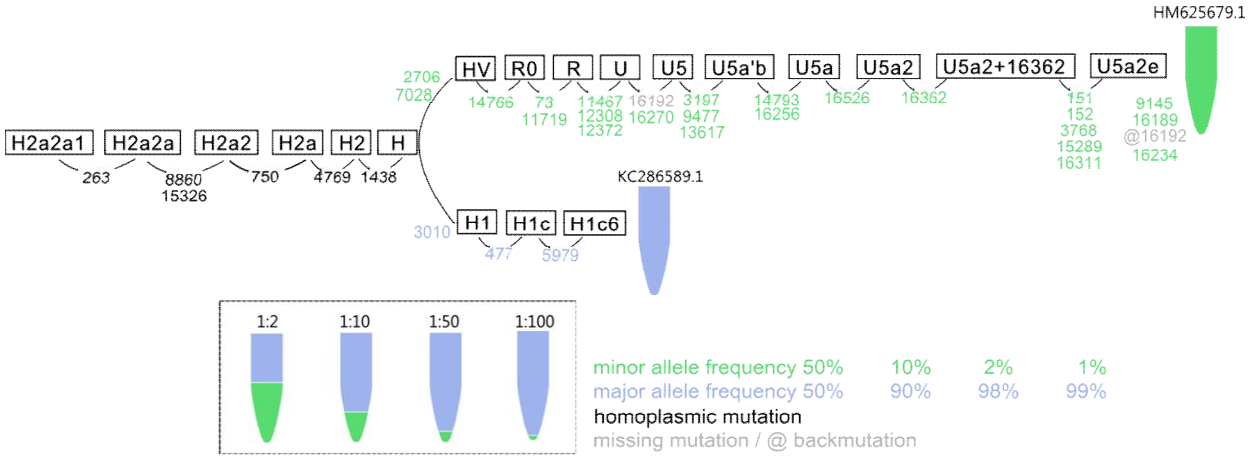
\includegraphics[width=1\textwidth]{images/mix-ups.png}
    \caption[Sample mixtures in the lab]{Two samples HM625679.1 and KC286589.1 as mixed in the lab. The profile of HM625679.1 (green) gets diluted down to 1\% level in the lab. The sites correspond the rCRS, and are either heteroplasmic (green or blue) according the mixture level or homoplasmic (=black, shared by both profiles, and expected as full base substitutions according the rCRS)} 
    \label{fig:mtdna-mix-ups}
\end{figure}
The Illumina HiSeq 2500 run yielded a mean coverage of 50,000x over the 6 samples (2 un-mixed and the 4 mix-ups) with a raw file size of the FASTQ files of 2GB per sample. The Ion Torrent PGM generated data on the Ion 318 Chip with a mean coverage of 5,000 fold over the same samples, with a BAM file size of 100MB per sample, already mapped with the Ion Torrent Suite. We converted the BAM files back to FASTQ files, for better comparison of the two devices, to exclude the impact of different mappers on the result. Both sets of files were run with the same parameters on mtDNA-Server and the results compiled based on comparing the expected to the detected heteroplasmic sites. For this purpose we determined the sensitivity (or recall) \textit{true positives rate}, the specificity (true negatives rate) and the precision (\textit{positive predictive value}). Listing \ref{eq:sensitivity} represents the definitions of the used performance metrics. 
\begin{equation}\label{eq:sensitivity}
\begin{split}
  Sensitivity =  \frac{number\ of\ true\ positives}{number\ of\ true\ positives\ + number\ of\ false\ negatives}\\ \\
  Specifity =  \frac{number\ of\ true\ negatives}{number\ of\ true\ negatives\ + number\ of\ false\ positives}\\  \\
  Precision = \frac{number\ of\ true\ positives}{number\ of\ true\ positives\ + number\ of\ false\ positives}
\end{split}
\end{equation}
The first validation was performed by comparing the Illumina HiSeq files after mapping with the same version of BWA MEM 0.7.5 to LoFreq, which is able of ultra-sensitive variant detection. Table \ref{table:illumina} shows the result based on the metrics presented for the Illumina HiSeq data. Table \ref{table:pgm} highlights the results for the Ion Torren PGM data.
\begin{table}[h]
\centering
\caption{Performance comparison between mtDNA-Server and LoFreq on the Illumina HiSeq 2500 mtDNA data}
\label{table:illumina}
\begin{tabular}{l|lll|lll}
\multicolumn{5}{c}{mtDNA-Server} &    {LoFreq} \\
\hline
\begin{tabular}[c]{@{}l@{}}Illumina\\ mix-up \end{tabular}  &  $Precis.$ & $Sensitiv.$ & $Specif.$  &  $Precis.$ &  $Sensitiv.$ & $Specif.$ \\
\hline
1:2 &   \textbf{100\%} &  \textbf{100\%}  & \textbf{100\%} &   93.1\%  & \textbf{100\%}   &   99.9\% \\
1:10 &  \textbf{100\%} &  \textbf{92.6\%}  & \textbf{100\%} &  89.3\%   &  \textbf{92.6\%}  &   99.9\% \\
1:50 &  \textbf{100\%} &  \textbf{92.6\%}  & \textbf{100\%}&   82.8\%  &  88.9\%  &   99.9\% \\
1:100 & \textbf{100\%} &  85.2\%  & \textbf{100\%} &  83.9\%   & \textbf{96.3\%}   &  99.9\%   
\end{tabular}
\end{table}
\begin{table}[h]
\centering
\caption{Performance comparison between mtDNA-Server and LoFreq on the Ion Torrent PGM mtDNA data}
\label{table:pgm}
\begin{tabular}{l|lll|lll}
\multicolumn{5}{c}{mtDNA-Server} &    {LoFreq} \\
\hline
\begin{tabular}[c]{@{}l@{}}PGM\\ mix-up \end{tabular}  &  $Precis.$ & $Sensitiv.$ & $Specif.$  &  $Precis.$ &  $Sensitiv.$ & $Specif.$ \\
\hline
1:2 &   \textbf{100\%} &  \textbf{88.89\%}  & \textbf{100\%} &  \textbf{100\%} & 81.48\%   &   \textbf{100\%} \\
1:10 &  \textbf{100\%} &  \textbf{81.48\%}  & \textbf{100\%} &  \textbf{100\%}  &  \textbf{81.48\%}   &   \textbf{100\%} \\
1:50 &  \textbf{100\%} &  \textbf{77.78\%}  & \textbf{100\%}&   \textbf{100\%} &  55.56\% &   \textbf{100\%} \\
1:100 & \textbf{100\%} &  \textbf{59.26\%}  & \textbf{100\%} &  \textbf{100\%}  & 11.11\% &  \textbf{100\%}   
\end{tabular}
\end{table}

As can be seen from the results, mtDNA-Server yields results that are more conservative: rather than finding all false negatives, it has the advantage of finding no false positives in this validation. The lack of not finding the true negatives relates to the BAQ which is applied as default in mtDNA-Server, which in this specific experiment shows some drawbacks. The diluted sample Lab002 shows 2 point mutation on site 151 and 152, as well as in the C-stretch around 16189 which are filtered too rigorously. On the other hand, LoFreq detects more false positives in the Illumina runs and even more false negatives in the PGM runs. In conclusion, both methods show a similar level of specificity and precision, but mtDNA-Server is slightly outperforming LoFreq regarding the sensitivity on both data sets from the NGS devices under investigation. This can come to additional costs if heteroplasmic variants are reassessed with a different method, for instance with Droplet Digital PCR or the Sequenom Platform, able to analyze specific sites, where the primers need to be known. 
\subsection{Pipeline Performance Comparison }
For comparison with the presented tools in the related work section, two independent data sets were analyzed again with LoFreq and additionally with mit-o-matic, MToolBox, Galaxy Naive Variant Caller and  MitoSeek. The evaluation accessed the heteroplasmic sites found per tool. The evaluation shows that mtDNA-Server is the most accurate heteroplasmic variant calling pipeline over the analyzed data sets, with perfect precision, indicating the least false positive hits are found with the herein described method.

Since the mix-ups generated in the lab, that we used for validation were too large for upload on most of the different tools, we used two smaller publicly available data sets. The first was the high and low coverage data for sample HG00096 from the 1000 Genomes Project Phase 1, the second was a tumor/benign sample pair from the Cancer Genome Atlas \cite{Chang2013}, presented in \cite{Guo2013}.

The following parameters were used for the evaluation in order to reproduce the results:
\begin{enumerate}


\item MitoSeek (version 1.3)
\begin{lstlisting}
perl mitoSeek.pl -i <input.bam> -t 4 -sb 0 -hp 1 -d 5 -str 4 -sp 1 -sa 0
\end{lstlisting}
\item MToolBox on MSeqDR
\begin{lstlisting}
Input format: BAM 
reference sequence: hg19+rCRS 
Filtering and extra option: none 
Minimum distance of ins/dels from read end: 5 bps
Heteroplasmy threshold for FASTA consensus sequence: 0.8
\end{lstlisting}
\item Galaxy Naive Variant Caller
\begin{lstlisting}
Minimum base quality =20
Minimum mapping quality = 20
Minimum number of reads needed to consider a REF/ALT needed = 20 
ploidy = 1
\end{lstlisting}
\item Mit-o-matic\\
The files were converted to the required FASTQ format with BEDTools \cite{Quinlan2010} BamToFastq prior analysis.
\begin{lstlisting}
Read length: 101, 
Data: SingleEnd,
Alignment Tool: BWA
Heteroplasmy cut-off: 10% (default) as well as 1% 
\end{lstlisting}
For HG00096 which was too big for upload (exceeding the 25MB upload limit), we used the command-line version with the following parameters:
\begin{lstlisting}
perl mitomatic.pl -c -t bwa -o se -f 10 -d hg00096_10 -i HG00096.fastq
\end{lstlisting}
\item LoFreq
 \begin{lstlisting}
lofreq call HG00096.bam -o HG00096.vcf -f rCRSreference.fasta
\end{lstlisting}
\item  MitoBamAnnotator\\
Unfortunately we were not able to run either of the samples on MitobamAnnotator, ending up with a timeout of the server.
\item \textbf{mtDNA-Server}:
For mtDNA-Server no further parameters needed to be adjusted.
\end{enumerate}

\begin{table}[h]
\centering
\caption[Expected and detected heteroplasmic variants in sample HG00096]{Expected and detected heteroplasmic variants in sample HG00096 for different tools. Mutations with bold number are expected. Transversions only found on one strand are considered as artefacts and marked with $\star$. Error hot spot mutations reported by Li et al. \cite{Li2010} are marked with $\star \star$. }
\label{table:hg00096}
\begin{tabular}{c|c|cccccc}
\hline
Mutation & Exp. & LoFreq & \begin{tabular}[c]{@{}l@{}}Gal\\ axy\end{tabular} & \begin{tabular}[c]{@{}l@{}}Mito\\ Seek\end{tabular} & \begin{tabular}[c]{@{}l@{}}MTool\\ Box\end{tabular} & \begin{tabular}[c]{@{}l@{}}Ye\\ et al\end{tabular} & \begin{tabular}[c]{@{}l@{}}mtDNA\\ -Server\end{tabular} \\
\hline
1456 T/C & \textbf{1.0\%} & & & & 1.2\% & & 1.0\%\\
2746 T/C & \textbf{1.8\%} & 2.3\% & 2.5\% &2.4\% & 2.4\% & 2.3\% & 2.5\%\\
3200 T/C &\textbf{0.9\%} & & & & 1.00\% & & 1.02\%\\
12410 A/G & \textbf{1.0\%} & 1.3\% &1.3\%  & 1.2\% & 1.0\% & & 1.1\%\\
14071 A/G &\textbf{1.0\%} & 1.0\% & 1.2\% & & 1.2\%& & 1.1\%\\
14569 G/A &\textbf{50.2\%} & 57.6\% & 57.7\% & 58.0\% & 59.3\% &56.2\%& 57.6\% \\
15463 A/G & \textbf{0.9\%} & & & & 1.3\% & 1.08\% &1.3\%\\
16093 T/C& \textbf{56.8\%} & 60.2\% & 60.9\% & & 60.2\% & 59.5\% &59.6\% \\
16360 C/T &\textbf{39.4\%} & 39.4\% & 38.8\%& &  39.5\% & 37.8\% &38.6\% \\
3488 T/A$\star$ & & & & 1.1\% & 1.1\% &  \\
6419 A/C$\star$  & &  & 4.5\% & 1.5\%& 1.7\% \\
10306 A/C $\star \star$& & & 6.3\% & 2.5\% & 1.8\% &  \\

\end{tabular}
\end{table}
For the validation purpose we analyzed the sample HG00096 high coverage ($\sim$ 15,000 x) as our gold standard with LoFreq (column Exp. in Table \ref{table:hg00096}) and compared the results with the low coverage data (mean coverage 1,300x) to LoFreq, Galaxy Naive Variant Caller, MitoSeek, MToolBox on MSEQDR, the result as presented in Ye et al. \cite{Ye2014} and mtDNA-Server.  Mit-o-matic resulted in over 528 heteroplasmic sites by applying a 1\% heteroplasmic threshold and  20 heteroplasmic sites with a 10\% threshold, with a wrong resulting haplogroup U8b1b1 instead of the expected H16a1 and was therefore excluded.\\

As a next validation, a pair of mtDNA sequences from an exome sequencing study of a benign/tumor Breast cancer sample from  the Cancer Genome Atlas \cite{Chang2013} was assessed (sample TCGA-BH-A0BM-01A-11W-A071-09 = brca\_tumor with a mean coverage of 200x and TCGA-BH-A0BM-10A-01W-A071-09 = brca\_benign with a mean coverage of 50x).
Figure \ref{fig:coverage_brca} shows the coverage plots directly generated in mtDNA-Server. With the two low coverage data presented, the variant calling is more error prone to artefacts and errors from the NGS devices and therefore presents a good comparison basis. 
\begin{figure}[!ht]
    \centering
    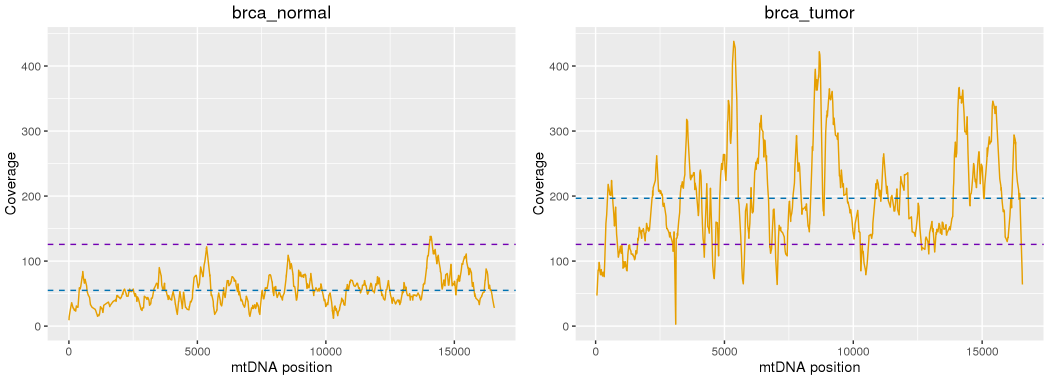
\includegraphics[width=1\textwidth]{images/coverage-brca.png}
    \caption[Coverage-plot generated by mtDNA-Server ]{Coverage-plot generated by mtDNA-Server of the two samples brca\_normal and brca\_tumor. The dotted line in purple shows the mean coverage over all analysed samples. The dotted line in turquoise shows the mean coverage for this specific sample.}
    \label{fig:coverage_brca}
\end{figure}
After analyzing the samples on mit-o-matic, Galaxy Naive Variant Caller (Galaxy NVC), LoFreq, MToolBox and mtDNA-Server the precision (Prec.) and sensitivity (Sens.) and specificity (Spec.) were estimated for both Samples. Table \ref{table:brca} represents the results of the metrics. In order to estimate the values, the results from LoFreq were used as the gold-standard, however ignoring the heteroplasmic variant on 10306 A/C which was shown to be an error hot spot by Li et al. \cite{Li2010}. 

\begin{table}[h]
\centering
\caption{Precision and Sensitivity based on the tumor-benign Breast-Cancer sample}
\label{table:brca}
\begin{tabular}{l|lll|lll}
\multicolumn{5}{c}{brca\_normal} &   {brca\_tumor}  \\
\hline
Pipeline &  $Prec.$ & $Sens.$ & $Spec.$  &  $Prec.$ & $Sens.$ & $Spec.$ \\
\hline
Galaxy NVC &    100\% &  100\% &  100\%  &   100\% &  62.5\% &  99.9\% \\
mit-o-matic &   0.17\% &  100\% &  99.9\%  &   71.4\% & 62.5\% & 99.9\% \\
MToolBox &      100\% &  100\% &  100\%  &   100\% & 100\% & 100\%\\
MitoSeek&       0\% &  0\% &  99.9\%  &   0\% & 0\% & 99.9\%\\
mtDNA-Server &  100\% &  100\% &  100\%  &   100\% &   100\% &   100\% \\
\end{tabular}
\end{table}
Detailed information on the variants found with each pipeline are provided in the Supplemental Material of the paper\footnote{\url{http://nar.oxfordjournals.org/content/suppl/2016/04/15/gkw247.DC1/SupplementaryMaterial.pdf}}. This evaluation again shows the poor performance of mit-o-matic, and surprisingly shows that a naive variant calling as performed with Galaxy is outperforming it. MToolBox and mtDNA-Server show similar results as LoFreq. MToolBox found additional 3 heteroplasmic variants that could be contributed to length heteroplasmy. But without further investigating the positions, they were not considered in this validation. 
\subsection{Scalability}
For the performance of the scalabilty mtDNA-Server was tested with an increasing amount of data size. Testing the scalability of the other pipelines is quite challenging, since often no batch processing is supported and samples can be only uploaded using a web interface. We performed two tests, one starts the whole steps with the Input of FASTQ files, the second test is with the BAM files from 1000 Genomes Project Phase 3. 

\subsubsection{Testing FASTQ paired-end (PE) samples}
High Coverage Illumina data (Illumina HiSeq 2500) from an in-house study \cite{Kloss-Brandstatter2015} with a mean coverage of $\sim$ 35,000 fold where used to validate the performance for the distributed alignment.
mtDNA-Server automatically detects paired-end data and adds an alignment step based on BWA-MEM 0.7.5. The Cluster Setup comprised a 3 Nodes Hadoop MapReduce Cluster with 30 CPUs in total and 2GB RAM per Node.
\begin{table}[h]
\centering
\caption{mtDNA-Server wall-time for FASTQ samples}
\label{table:fastq}
\begin{tabular}{lll}
Number of Samples  &  Datasize & Execution Time \\
\hline
10 &   6.2 GB &  30 min 10 sec \\
20 &  12 GB &  56 min 37 sec   \\
40 &  19 GB &  2 h 9 min 39 sec  \\
80 & 36 GB &  4 h 5 min 21 sec   
\end{tabular}
\end{table}

When taking a closer look at the run with the 80 FASTQ paired-end samples, mtDNA-Server provides the information for each step in the workflow, as presented in listing \ref{list80fastq}  

\begin{lstlisting}[caption=Execution times of workflow-steps in analysis of 80 FASTQ samples with mtDNA-Server, label=list80fastq]
Align                             [1 h 19 min 29 sec]
Sort BAM                          [1 h 48 min 2 sec]
Analyse BAM                       [54 min 6 sec]
Detect Heteroplasmy               [28 sec]
Haplogroup Detection              [8 sec]
Haplogroup Contamination Check    [20 sec]
Report Creation                   [54 sec]
Sending Mail                      [2 sec]
\end{lstlisting}

\subsubsection{Testing 1000G Phase1 BAM data}	
Data (up to 800 samples) were downloaded from the European Bioinformatics Institute FTP Server\footnote\url{ftp://ftp.1000genomes.ebi.ac.uk/} including Illumina and Roche data, in order to check for the scalability. Samtools was used for the download, by limiting to the mitochondrial genome reads only. As represented in Table \ref{table:bam} and in Figure \ref{fig:scalability} mtDNA-Server scales well with the amount of BAM samples. 
\begin{table}[h]
\centering
\caption{ mtDNA-Server wall-time for 1000 G Phase 1 BAM data}
\label{table:bam}
\begin{tabular}{lll}
Number of Samples  &  Datasize & Execution Time \\
\hline
50 &   1.8 GB &  3 min 26 sec\\
100 &  3.5 GB &  5 min 48 sec  \\
200 &  6.9 GB &  10 min 25 sec  \\
400 & 14 GB &  20 min 9 sec \\
800 & 27 GB & 38 min 54 sec
\end{tabular}
\end{table}

\begin{figure}[!ht]
    \centering
    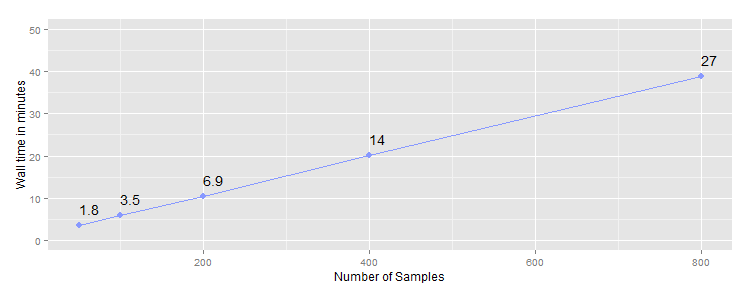
\includegraphics[width=1\textwidth]{images/scalability.png}
    \caption[Scalability of the mtDNA-Server pipeline]{Scalability of the Pipeline: Data from table \ref{table:bam} represented as x/y plot, where the points are denoted with the filesize in GB} 
    \label{fig:scalability}
\end{figure}
% DATA FOR PLOT IN R
% samples =c(50, 100, 200, 400, 800)
% size = c(1.8, 3.5, 6.9, 14, 27)
% df =data.frame(samples, size, timeMin)
% timeMin= c(3+(26/60), 5+(48/60), 10+(25/60), 20+(9/60), 38 + (54/60))
% ggplot(df, aes(x=samples, y=timeMin)) +  geom_line(aes(group=1), colour="#8899ff") +  geom_point(size=3, colour="#8899ff") +  xlab("Number of Samples") +  ylab("Wall time in minutes") + geom_text(aes(label=size),hjust=0, vjust=-1) +   ylim(0, 50) 

\section{Conclusion and Outlook}
In this chapter the "mtDNA-Server" (published in \cite{Weissensteiner2016b}) was described. It is a free and reproducible web service available on \url{http://mtdna-server.uibk.ac.at} for the complete mitochondrial NGS data analysis workflow, based on MapReduce. The focus is on the reliable detection of heteroplasmic variants as well as contamination in the samples. Complicated preprocessing steps are hidden to non-domain experts. The results highlight the accurate detection of variants (hetero- and homoplasmic) but also shows the scalability of the method with the increase amount of samples. mtDNA-Server has been developed in cooperation with the University of Michigan (Center for Statistical Genetics), the Medical University of Innsbruck and the University of Innsbruck, Institute of Computer Science with the Group of Database and Information Systems also providing the Hardware for this service.
Two important aspects need to be considered when providing such a free service:
\begin{enumerate}
\item Scalability of the service: All computational intensive steps are parallelized with Hadoop MapReduce and executed graphically with the Hadoop framework Cloudgene \cite{Schonherr2012, Weissensteiner2016b}. This framework is also used as the underlying framework for a heavily used service, the Michigan imputation Server \cite{Das2016} with over 10 million imputed genomes\footnote{\url{https://imputationserver.sph.umich.edu} accessed May 2017}.
\item Data Sensitivity: A wide array of security measures are in force \cite{Weissensteiner2016a}. Both data for input and output is removed from our servers as soon it is no longer needed. To upload and download data, users must register with a unique e-mail address and strong password or store the encrypted token URLs only accessible by the user who uploaded the data. Users can only download results for samples that they have uploaded; no other server users will be able to access their data.
\end{enumerate}

As of May 2017 over 45,000 samples got processed from scientists around the world and more than 400 users registered on the site. User registration is however not demanded to submit jobs. There's some more work to be addressed in the near future:

 Currently mtDNA-Server is focusing on the point mutations only. Insertions and deletions are not considered in the current version. This will be implemented in the near future (deletions are already emitted in the pileup file).
 
 Annotation of the heteroplasmic sites will be extended to phylogenetic scores and some pathogenicitiy scores, as already done in the homoplasmic variants. 

VCF file support, which should allow export of this file. While there is no current standard on how to write heteroplasmic variants, the VCF format presented in \cite{Calabrese2014} can be supported.

Since many researchers are not allowed to upload data to a remote destination we also plan on providing a Docker Image\footnote{\url{https://www.docker.com/}} for local usage. This allows to provide incremental updates to all users.  









\cleardoublepage
\chapter{Detecting Contamination in massive parallel sequencing studies}
\label{chapterContamination}
With the new technological progress that comes with the DNA sequencing based on massive parallel sequencing, there are however also some drawbacks. The shorter read-length compared to Sanger-based Sequencing can be targeted with the so called Third Generation Sequencing, with new companies like Oxford Nanopore Technologies\footnote{\url{nanoporetech.com}}, Pacific Biosciences\footnote{\url{http://www.pacb.com/}} or BioNano Genomics\footnote{\url{http://bionanogenomics.com/}} already conquering the market for sequencing devices. Another issue, that becomes more prevalent, is the immanent issue of contamination, based on the very sensitive NGS technology. While Sanger based Sequencing is able to detect heteroplasmic variants down to the 10\% level for the minor allele \cite{Kloss-Brandstatter2015}, NGS can detect heteroplasmic variants down to the 1\% minor allele level and even lower \cite{Li2010}. Also the expanding amount of sequencing studies increases the probability of errors to occur. The error can come in many forms in the lab, but also in the data processing steps. While in the lab or while sequencing, sample contamination, cross-species contamination, carry-over contamination from previous run, issues with PCR products, issues with fragmentation of DNA, wrong protocols and many more can become problematic. The post-processing from the raw sequencing reads to the annotated variants can also lead to errors, due to wrong methods applied, with the wrong parameters, wrong reference sequences in use (this is especially the case for mitchondrial sequencing studies where different reference sequences are in use \cite{Behar2012,Andrews1999} or systematic errors as previously described (see phantom mutations \ref{hg:phantom}). One option to avoid post-processing errors, is the use of automated pipelines, reducing the risk such issues. Quality control is a second important option. Therefore in this chapter the concepts described in Chapter \ref{chapterHaplogrep} and Chapter \ref{chap:NGS} get combined to check mitochondrial data derived from massive parallel sequencing for the presence of contamination, based on low-level heteroplasmy that can be used to help identifying an extra haplogroup in the sample of interest (see section \ref{haplochecker}. The concept was drafted in Li et al \cite{Li2010} based on manual inspection with Phylotree as well as in Avital et al \cite{Avital2012} by taking advantage of HaploGrep. A recent discussion highlights the problem of contamination in mitochondrial NGS studies \cite{Ye2014,Just2014, Just2015,Ye2014reply} and tools for detection of contamination are emerging \cite{Renaud2015,Jun2012,Dickins2014}, as presented in the related work section \ref{cont:relatedwork}. The performance of the new workflow called HaploChecker is presented in the Results section \ref{cont:result}, and the method is abstracted in the last section \ref{cont:outlook}, by highlighting future applications as well as opportunities for improvements.

\section{Related Work}\label{cont:relatedwork}
The need for a quality check of sequencing data has been addressed in the past for Sanger based data \cite{Walker2004, Montesino2007, Bandelt2009, Yao2007} as well as for NGS based data \cite{Holland2011}. 
Concepts for detecting and correcting contamination were presented for nuclear DNA NGS sequencing projects, where MicroArray data are available were presented in Jun et al. \cite{Jun2012} and Flickinger et al. \cite{Flickinger2015} respectively. The provided application \textbf{VerifyBamId}\footnote{\url{http://genome.sph.umich.edu/wiki/VerifyBamID}} is applying likelihood-based methods for detecting sample contamination based on sequence and MicroArray-based genotype data \cite{Jun2012}. This approach was applied on all samples from the 1000 Genome data set, and the resulting data release Phase 1 and Phase 3 were filtered accordingly the contamination-index provided by VerifyBamID. 

A recent approach was presented by Dickins at al. \cite{Dickins2014} by describing a Galaxy \cite{Goecks2010,Afgan2016} based pipeline for contamination control in mitochondrial genomes. The pipeline as well as the data are available through the website\footnote{\url{https://usegalaxy.org/u/aun1/p/controlling-for-contamination-in-resequencing}}. An advantage of this tool is the Galaxy related reproducibility of the workflow\footnote{\url{https://usegalaxy.org/u/aun1/p/controlling-for-contamination-in-resequencing}}. The concept of the method is based on building a Neighbor-Joining (NJ) tree \cite{Saitou1987}, for the minor allele frequency (MAF). The method is based on the assumption that contamination is manifested in a sample by multiple polymorphic sites with tight MAF distribution. The provided workflow is straightforward in small to large scale data sets such as in population studies. While this approach can have advantage over a haplogroup-based detection of contamination in some situations, it is not suitable for investigations on single profiles which accounts in particular for forensic investigations but also for case studies in medical research. Further the source of contamination is required to be present in the data set, often not feasible.

A further different approach is presented in the tool called \textbf{Schmutzi} by Renaud et al. \cite{Renaud2015}, for detecting contamination in ancient mitochondrial DNA samples. Based on empirical and simulated data sets, the contamination estimation tool is designed for highly degraded mtDNA also affected by cytosine deamination (loosing an amine group from the molecule, being  a process typical in ancient DNA) and problems with contamination with present day DNA.  However, the absence of deamination yields incorrect estimations and therefore their tool is highly recommended to be used exclusively on mtDNA harbouring the mentioned properties. The underlying framework is based on a Bayesian maximum a posteriori algorithm, which yields the most likely model parameters from the provided data. 

While the presented related tools are designed for different NGS derived data, the comparison with our new method is performed on two different data sets. For comparison with the mitochondrial NGS data, we compare the data set provided by Dickins et al. \cite{Dickins2014} to check if the haplogroup-based contamination check presented subsequently can detect the expected contamination described. We further demonstrate the use of our approach in the 1000 Genomes phase 3 data set, including 2,504 whole genome sequences from 26 populations world wide. A direct comparison with the tool from Renaud et al. could not be performed.


\section{mtDNA phylogenetic approach for contamination control}\label{haplochecker}
We developed a tool for mitochondrial sequence data analysis for estimation of contamination accessible via http://mtdna-server.uibk.ac.at/start.html and as a standalone version on Github https://github.com/haansi/greenVC. The underlying principle is that all mitochondrial variants relative to the mitochondrial reference sequence rCRS \cite{Andrews1999} can be split into minor and major variant allele frequency (VAF), as suggested by Li et al. \cite{Li2010} and Avital et al. \cite{Avital2012}.
\subsection{Naive Variant Caller}
While the method presented in Chapter \ref{chap:NGS} directly implements the approach presented in \ref{cont:haplochecker}, it was not designed for the purpose of detecting low-level contaminations in low-coverage data, but rather detect reliably the presence of homo- and heteroplasmic variants. To detect contamination below the 10\% level in sequence data with a coverage $<$ 100 fold, a naive variant caller was designed, based on the HTSJDK framework\footnote{\url{https://samtools.github.io/htsjdk/}}, and applies a Clopper Pearson binomial confidence interval \cite{CLOPPER1934}, representing an exact confidence interval. The number of minor alleles (x), the coverage (n) and the confidence level ($\alpha$) are provided, such that the lower limit ($ll$) and upper limit ($ul$) are provided:
\begin{equation}
 ll = \frac{1}{(1 + \frac{(n - x + 1)}{(x qf(\frac{\alpha}{2}, 2 x, 2 (n-x+1)))})}
\end{equation}
\begin{equation}
 ul = \frac{1}{(1 + \frac{(n - x)    }{ ((x + 1)  qf(1-\frac{\alpha}{2}, 2 (x+1), 2 (n-x)))})}
\end{equation}
For $x=0$ yields $ll=0$ and $ul = 1 - (\frac{\alpha}{2})^{(\frac{1}{n})}$ and for $x = n$ $ll = \frac{\alpha}{2}^{(\frac{1}{n})}$, and $ul =1$. Since those two exceptions represent homoplasmic variants (either all bases according the reference or all bases as complete exchange), the calculation can be omitted.
The quantile function $qf$ accepting the quantile parameters for the F-distribution ( $ll_{\alpha} = \frac{\alpha}{2}$ and $ul_{\alpha}= 1-\frac{\alpha}{2}$ respectively) and the degrees of freedom ($ll_{df_1} = 2x$, $ll_{df_2} = 2 (n-x+1)$,  $ul_{df_1} =  2 (x+1)$, $ul_{df_1} =  2 (n-x)$ ) \footnote{\url{https://stat.ethz.ch/R-manual/R-devel/library/stats/html/Fdist.html}}. A heteroplasmy is marked as reliable, when the lower limit exceeds the user defined threshold $h_T$ ($ll  \geq h_T$). The Clopper-Pearson implementation from the Apache Commons Mathematics Java Library\footnote{\url{http://commons.apache.org/proper/commons-math}} is applied.
\begin{enumerate}
\item \textbf{bam2var}: a user defined quality score filtering is applied, and all reads with read length $>$ 20 bases are considered. Reads are handled in such manner, that the circular structure of the mtDNA is considered, and positions exceeding the length of the user-provided reference restart at base 1. 
The parameters are the BAM input file (in), the result folder (out), where the pileup file as well as the variant file and haplogrep input files are generated, the reference sequence (ref), the variant allele frequency (VAF), applied to distinguish between heterop, and homoplasmic variants and the base quality (QUAL). The listing shows an example, VAF corresponding to 20\% here:
\begin{lstlisting}[language=bash]
java -jar greenVC.jar bam2var --in HG01500.IBS.exome.MT.bam --out resultfolder  --ref data/rcrs.fasta  --VAF 0.2 --QUAL 20
\end{lstlisting}
\item \textbf{haplocheck}: generation of the haplogrep input files for contamination detection. The method is presented in \ref{cont:haplochecker}. This command writes based on the previous called variants to a haplogrep input file, by splitting it in major/ minor allele profiles in order to check for sample contamination down to the 5\% heteroplasmic level.
\begin{lstlisting}[language=bash]
java -jar greenVC.jar haplocheck --in resultfolder/variants.txt --out haplogrepinput.hsd   --VAF 0.05 
\end{lstlisting}
\item \textbf{haplocheck-mtDNA-Server}: the result in the heteroplasmies.txt file from mtDNA-Server (see Chapter \ref{chap:NGS}) is handled similar to the \textbf{haplocheck} option. Again, the input file is assigned major/ minor allele profiles in order to check for sample contamination with HaploGrep \ref{chapterHaplogrep}. Example call:
\begin{lstlisting}[language=bash]
java -jar greenVC.jar haplocheck-mtDNA-Server --in heteroplasmies.txt --out haplogrepinput.hsd  --VAF 0.05 
\end{lstlisting}
\item \textbf{lofreq}: the resulting VCF file, generated by LoFreq \cite{Wilm2012}, as an additional ultra-sensitive variant caller (able of calling variants occurring in <0.05\% of all reads) can further be used as data input. The htsjdk-library\footnote{\url{https://github.com/samtools/htsjdk}} is applied here to read the VCF file, and transforming the information provied to HaploGrep input profiles. LoFreq itself does not call genotypes\footnote{\url{http://csb5.github.io/lofreq/}}, so the SAMPLE and FORMAT columns in the VCF file are missing.The required information for the generation of HaploGrep files, are the vcf filename, the position, the reference and the alternative base, as well as the allele frequency, provided in the INFO
\begin{lstlisting}[language=bash]
java -jar greenVC-0.1.jar lofreq --in inputfile.vcf --out haplogrepinput.hsd 
\end{lstlisting}
\item \textbf{GUI}: the application has a simple Swing GUI, shown if no parameter is provided. The bam2var step is calculated based on the parameters previously described.
\end{enumerate}
The presented method requires manual inspection of the HaploGrep results, while this is not explicitly the case for the pipeline presented thereafter. 
\subsection{HaploChecker}\label{cont:haplochecker}
Haplochecker starts with the called pileup variant file, with the variants in tab-spaced fileformat. Shared homoplasmic mutations help identifying the source of contamination, indicating mutual variants along phylogenetic branches. The contamination detection approach is also implemented directly in mtDNA-Server pipeline as drafted in Chapter \ref{chap:NGS} for FASTQ or BAM files. On the web interface again generated by Cloudgene, files for upload are requested to include the following indications: Sample ID (ID), mtDNA Position (POS), Major Allele (WTALLELE), Variant Allele (MUTALLELE) and the minor variant allele frequency (VAF). The threshold for heteroplasmy level detection is user defined and is employed to differentiate between heteroplasmic and homoplasmic variants. After the file upload is performed, HaploGrep  profiles are generated directly in the pipeline by separating the minor and major component of a heteroplasmic variant accordingly to the resulting profiles (Figure ). HaploGrep is based on the constantly updated worldwide mtDNA phylogeny Phylotree of currently 5,437 haplogroups. The generated profiles are subsequently checked for haplogroup (hg) consistency. The generated report indicates possible contaminations based on phylogenetic differences. Figure \ref{cont:workflow} represents the overview of this workflow. It is possible to provide both either heteroplasmic and homoplasmic sites or heteroplasmic sites only. The differing haplogroup affiliations of major and minor component are reported per sample along with a score value indicating the following additional information: a) heteroplasmies found in the resulting haplogroup, b) positions not covered under this haplogroup affiliation, c) heteroplasmies not showing any impact on the current phylogeny (either according the rCRS or never observed in Phylotree 17) (global private mutations) or heteroplasmiesic variants found in other haplogroups (local private mutations). For all polymorphisms found in the resulting haplogroup, the standard deviation and the mean value of the VAF of heteroplasmic mutations are calculated, and the results are represented as boxplots (see Appendix). 
\begin{figure}[!ht]
    \centering
    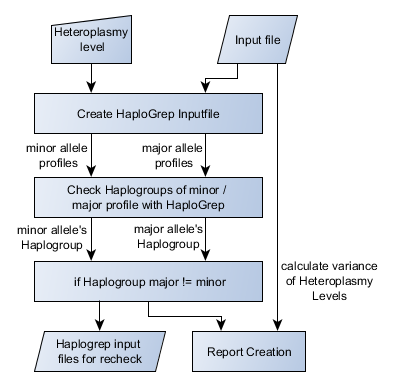
\includegraphics[width=0.8\textwidth]{images/dataflow.png}
    \caption[Pipeline for contamination detection]{Pipeline for contamination detection } 
    \label{cont:workflow}
\end{figure}

 
\section{Results}\label{cont:result}
The pipeline was defined as a YAML file for the generation of the Cloudgene based workflow, abstracted in the Figure \ref{cont:workflow}. The workflow joins two JAR files, one for the generation of the HaploGrep profiles and the second representing a console version of HaploGrep, as well as the logic for contamination detection directly implemented in R, accepting the HaploGrep result files, and the input files for the generation dynamic html report, based on R Markdown. 
The download of the chromosome MT BAM files resulted in a data volume of 97 GB. In total 2,504 samples were analyzed, as inferred from the sample information provided on the public available sample information (see Supplemental Material for URL). Supplemental Table 1 displays the mapping statistics over all 2,504 samples. In total 1,174,564,365 reads were processed on mtDNA-Server with the previously described parameters yielding to 12,489 heteroplasmic sites over all samples, corresponding 4.98 heteroplasmies per sample. The frequency of the highest occurring mtSNPs is corresponding the expected hot spots in the mitochondrial genome – See supplemental Table 2. Heteroplasmies are manifested on 5,065 sites out of all possible 16,569 sites. 

\subsection{Validation}
The evaluation of Haplochecker  was performed using simulated data, where we randomly mixed haplotypes of known haplogroups in silico and generated test profiles. As contamination detection within haplogroup H (approximately 45\% within Europe) is critical due to the comparison or largely similar sequences according to the European reference (rCRS), we placed particular emphasis on the validation of sequences belonging to haplogroup H. Therefore, we mixed all neighboring samples assigned to haplogroup H (858) and again generated test profiles (see supplemental Materials). Subsequently, the major and minor profiles of the haplotypes were retrieved by assigning different variant allele frequencies for each shared, minor and major mutations. Shared mutations were denoted with VAF 1, major variants $>$0.5 and minor contributions $\leq$ 0.5), respectively. For these simulations, we used data of the most recent phylogeny based on Phylotree 17, comprising 4,560 variants (3,740 transitions, 399 transversions, 50 inserts, 50 deletions and 123 back mutations defining 5,435 haplogroups. 
\subsection{1000G phase 3 data}
The data previously described and processed by the pipeline shows several samples with a high number of heteroplasmic variants $\geq$ 20 sites. Large amount of those samples can be identifies as contaminated (see Figure \ref{cont:1000G}). What further gets visible in this experiment, is the coverage distribution over the 2,504 samples. A cluster becomes apparent that has a low coverage of $\leq$ 500x coverage. Since all data are generated by whole genome sequencing on the same vendor's devices, the coverage reflects the relative amount of mitochondrial copy number to the nuclear DNA. Taking the provided 1000G sample information into account, the variance in the mean coverage can be explained by the origin of the DNA extraction. Samples with DNA extracted from blood show a much lower mitochondrial copy number (mtCN) compared to samples where the DNA was extracted from the lymphoblastoid cell lines (LCL). The mitochondrial copy number is often calculated as $m$ or $mtCN$, by calculating the ratio between reads mapping to the mitochondrial genomes ($r_m$), to the reads which map to the nuclear genome ($r_n$)\cite{Reznik2016}.
\begin{equation}
mtCN = \frac{r_m}{r_n}
\end{equation}
Ding et al \cite{Ding2015} further take the two copies of autosomal DNA in the cell into account, by taking the average coverage of the mtDNA ($avgCov_m$) and the autosomal DNA ($avgCov_n$) into account:
\begin{equation}
mtCN = \frac{avgCov_m}{avgCov_n}\times{2}
\end{equation}
When making statements about the copy number derived in this manner, it is of extreme importance not to mix samples where different DNA extraction methods are applied.
\begin{figure}[!ht]
    \centering
    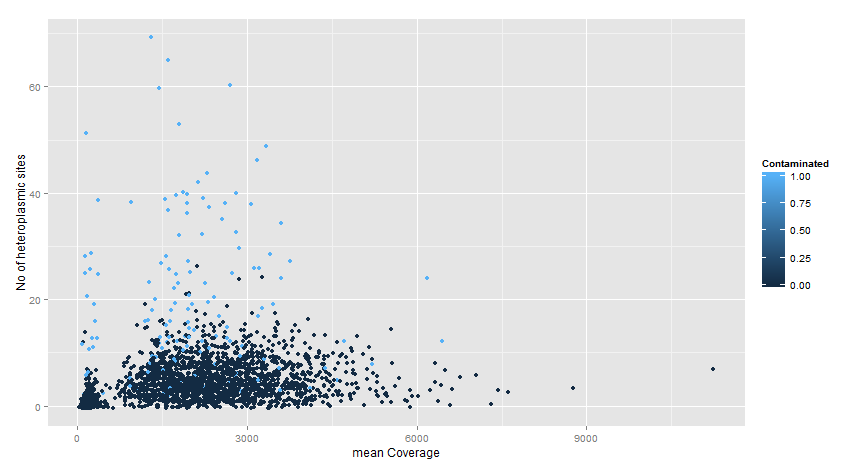
\includegraphics[width=1\textwidth]{images/contamination1000g.png}
    \caption[Contaminated Samples in 1000G phase 3]{Contaminated Samples in 1000G phase 3, the x-axis represents the mean coverage per sample, and the y-axis represents the amount of heteroplasmic sites per sample. The color indicates if a sample is affected by contamination.} 
    \label{cont:1000G}
\end{figure}
\subsection{Pipeline Performance Comparison}
While the direct comparison to the method from Renaud et al. \cite{Renaud2015} is not feasible for non-degraded DNA, the comparison to the Galaxy pipeline \cite{Dickins2014} as well as the VerifyBamId \cite{Flickinger2015} is represented in this subsection. The different setups for the comparison are the following: 
\begin{itemize}
\item The data represented in \cite{Dickins2014} was downloaded resulting in 13GB of paired end FASTQ files. The processing of the data was done with a private mtDNA-Server installation, and the samples were assessed for contamination with the herein presented method. Subsequently the results from Dickins et al were compared. Figure \ref{cont:family} summarizes the contaminated samples in the data provided by Table \ref{comptable} represents the results from the Galaxy Pipeline and the results from the contamination pipeline directly implemented in mtDNA-Server.
\begin{figure}[!ht]
    \centering
    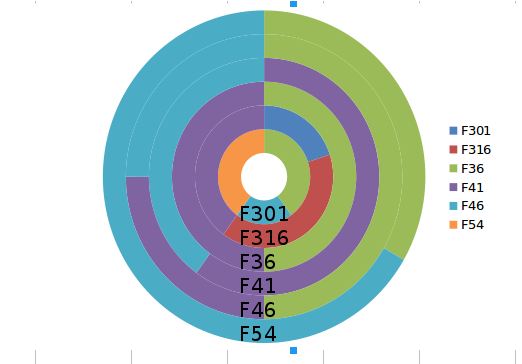
\includegraphics[width=0.7\textwidth]{images/families.png}
    \caption[Contamination represented in the Family mtDNA data]{Contamination represented in the Family mtDNA data  \cite{Dickins2014} analyzed with the herein described method regarding contamination. As can be seen, the different families F301 (n=5), F316 (n=5), F36 (n=6), F41 (n=5), F46 (n=4) and F54 (n=3) all show traces of contamination. Each circle represents a family, the color represented in the legend indicate what other DNA contributed the contaminations.} 
    \label{cont:family}
\end{figure}
\begin{table}[]
\centering
\caption{Comparison Galaxy pipeline to the contamination detection based on the known phylogeny implemented in mtDNA-Server. Total.Sites represents the heteroplasmic variants found in each sample, EVAL for the Galaxy Pipeline are classified in fail (contaminated), warn (possible contamination) and pass (no contamination). EVAL for mtDNA-Server lists a haplogroup, indicating the source of contamination if present, or empty, if the Total.Sites can not be assigned a minor profile. Samples highlighted in blue indicate the contaminated ones, samples in orange indicate conflicting results between the two pipelines.}
\label{comptable}
\begin{tabular}{lllll}
     & \multicolumn{2}{c}{\textbf{Galaxy}} & \multicolumn{2}{c}{\textbf{mtDNA-Server}} \\
\textbf{Sample}       & \textbf{Total.Sites}     & \textbf{EVAL}     & \textbf{Total.Sites}        & \textbf{EVAL}        \\
F301-M468-BL &35 &\cellcolor[HTML]{34CDF9} fail &30 &\cellcolor[HTML]{34CDF9}H3af \\
F301-M468C1-BL &40 &\cellcolor[HTML]{34CDF9} fail &45 &\cellcolor[HTML]{34CDF9}H3af \\
F301-M468C2-BL &47 &\cellcolor[HTML]{34CDF9} fail &47 &\cellcolor[HTML]{34CDF9}K2a10 \\
F301-M468C3-BL &33 &\cellcolor[HTML]{34CDF9} fail &51 &\cellcolor[HTML]{34CDF9}K2a10  \\
F301-M468C4-BL &39 &\cellcolor[HTML]{FFCC67}warn &64 &\cellcolor[HTML]{34CDF9}U2e2a1 \\
F316-M483-BL &38 &\cellcolor[HTML]{34CDF9} fail &65 &\cellcolor[HTML]{34CDF9}J1b1a1a \\
F316-M483C1-BL &41 &\cellcolor[HTML]{34CDF9} fail &46 &\cellcolor[HTML]{34CDF9}J1b1a1a \\
F316-M483C2-BL &25 &\cellcolor[HTML]{34CDF9} fail &31 &\cellcolor[HTML]{34CDF9}J1c1a \\
F316-M483C3-BL &8 &warn &3 & \\
F316-M483C4-BL &6 &warn &0 & \\
F36-M45-BL &5 &pass &1 & \\
F36-M45C1-BL &8 &warn &0 & \\
F36-M45C2-BL &7 &warn &3 & \\
F36-M45C3-BL &43 &\cellcolor[HTML]{34CDF9} fail &38 &\cellcolor[HTML]{34CDF9}J1b1a1a \\
F36-M45C4-BL &42 &\cellcolor[HTML]{34CDF9} fail &39 &\cellcolor[HTML]{34CDF9}J1b1a1a \\
F36-M46-BL &12 &\cellcolor[HTML]{34CDF9} fail &41 &\cellcolor[HTML]{34CDF9}J1b1a1a \\
F41-M51-BL &9 &warn &13 &\cellcolor[HTML]{FFCC67}J1b1a \\
F41-M51C1-BL &6 &warn &2 & \\
F41-M51C2-BL &7 &warn &2 & \\
F41-M52-BL &54 &\cellcolor[HTML]{34CDF9} fail &59 &\cellcolor[HTML]{34CDF9}U2e2a1 \\
F41-M52C1-BL &39 &\cellcolor[HTML]{34CDF9} fail &52 &\cellcolor[HTML]{34CDF9}U2e2a1 \\
F46-M57-BL &46 &\cellcolor[HTML]{34CDF9} fail &59 &\cellcolor[HTML]{34CDF9}J1b1a1a \\
F46-M58-BL &12 &warn &18 & \\
F46-M58C1-BL &43 &\cellcolor[HTML]{34CDF9} fail &36 &\cellcolor[HTML]{34CDF9}H3af \\
F46-M58C2-BL &35 &\cellcolor[HTML]{34CDF9} fail &36 &\cellcolor[HTML]{34CDF9}H3af \\
F54-M67-BL &37 &\cellcolor[HTML]{34CDF9} fail &32 &\cellcolor[HTML]{34CDF9}H3af \\
F54-M67C1-BL &44 &\cellcolor[HTML]{34CDF9} fail &58 &\cellcolor[HTML]{34CDF9}U2e2a1 \\
F54-M67C2-BL &42 &\cellcolor[HTML]{34CDF9} fail &51 &\cellcolor[HTML]{34CDF9}U2e2a1  \\       
\end{tabular}
\end{table}

\item The Phase 3 data released was verified with VerfifyBamID prior to publication by the 1000G consortium\footnote{\url{http://ftp.1000genomes.ebi.ac.uk/vol1/ftp/technical/working/20130514_phase3_verifybam_results/}}. For verifying the herein presented haplogroup based contamination detection approach, the mitochondrial sequences were downloaded from all samples marked with the verdicts \verb|HIGH_CHIP_MIX| (n=27), \verb|HIGH_FREE_MIX| (n=11) and \verb|POSSIBLE_SWAP| (n=7) from the FPT site \footnote{\url{ftp://ftp.1000genomes.ebi.ac.uk/vol1/ftp/data_collections/1000_genomes_project/data/}}. The data comprised 37 CRAM\footnote{http://www.ebi.ac.uk/ena/software/cram-toolkit} files (8 samples showed two verdicts), and was retrieved with the latest Samtools 1.3.1. In a second step the CRAM files were converted to FASTQ files and remapped with BWA MEM to the rCRS reference sequence. Thereafter all steps were identical to the analysis of the 1000G Phase 3 low coverage data described previously.
The file size of the samples accumulated to \~ 500 MB, varying significantly in size. The mean coverage over the mt-genome varies between \~100x (HG03982) and \~8,000x (HG03799). Out of the 3 different contamination classifications (\verb|HIGH_CHIP_MIX|, \verb|HIGH_FREE_MIX| and \verb|POSSIBLE_SWAP|), the sample contamination in \verb|HIGH_CHIP_MIX| could be confirmed in 26 / 27 samples, where HG01912 showed a coverage too low to predict reliable heteroplasmic sites in the lower percentage levels with mtDNA-Server. When analyzed with our naive variant caller (https://github.com/haansi/greenVC), the contamination in HG01912 could be confirmed (mixture of haplogroups L3 and L2c). The samples with the verdict \verb|HIGH_FREE_ MIX| could be confirmed in 8  out of 11 samples, where HG02524 and HG02525 showed a low mean coverage of 110x and 133x. Again by employing the naive variant caller, also the two low covered samples could be confirmed as contaminated. Sample HG04301 could not be confirmed as contaminated based on the mitochondrial DNA, although it showed a high coverage of 2,100x. The samplare combined to a workflow in the previous chapter. Samples marked as \verb|POSSIBLE_SWAP| did not show signs of haplogroup contamination.
\item Additionally all data from the 1000G phase 3 was classified in two groups: contaminated, and contamination free. Thereafter the mean scores for  \verb|HIGH_FREE_MIX| and \verb|HIGH_CHIP_MIX| for the Illumina Omni Chip and Affymetrix Microarray were taken into consideration. Samples, which were makred as contaminated by HaploChecker show higher mean scores, then the contamination free samples. The results are represented in Figure \ref{contScores}. The upper bound of 0.03 is the result of the prefiltering applied, based on which the data selection for the 1000G phase 3 data set was performed. The higher mean values of Contamination are as expected, indicating that the results from VerifyBamId, are in concordance between the different platforms Illumina and Affymetrix.
\begin{figure}[!ht]
    \centering
    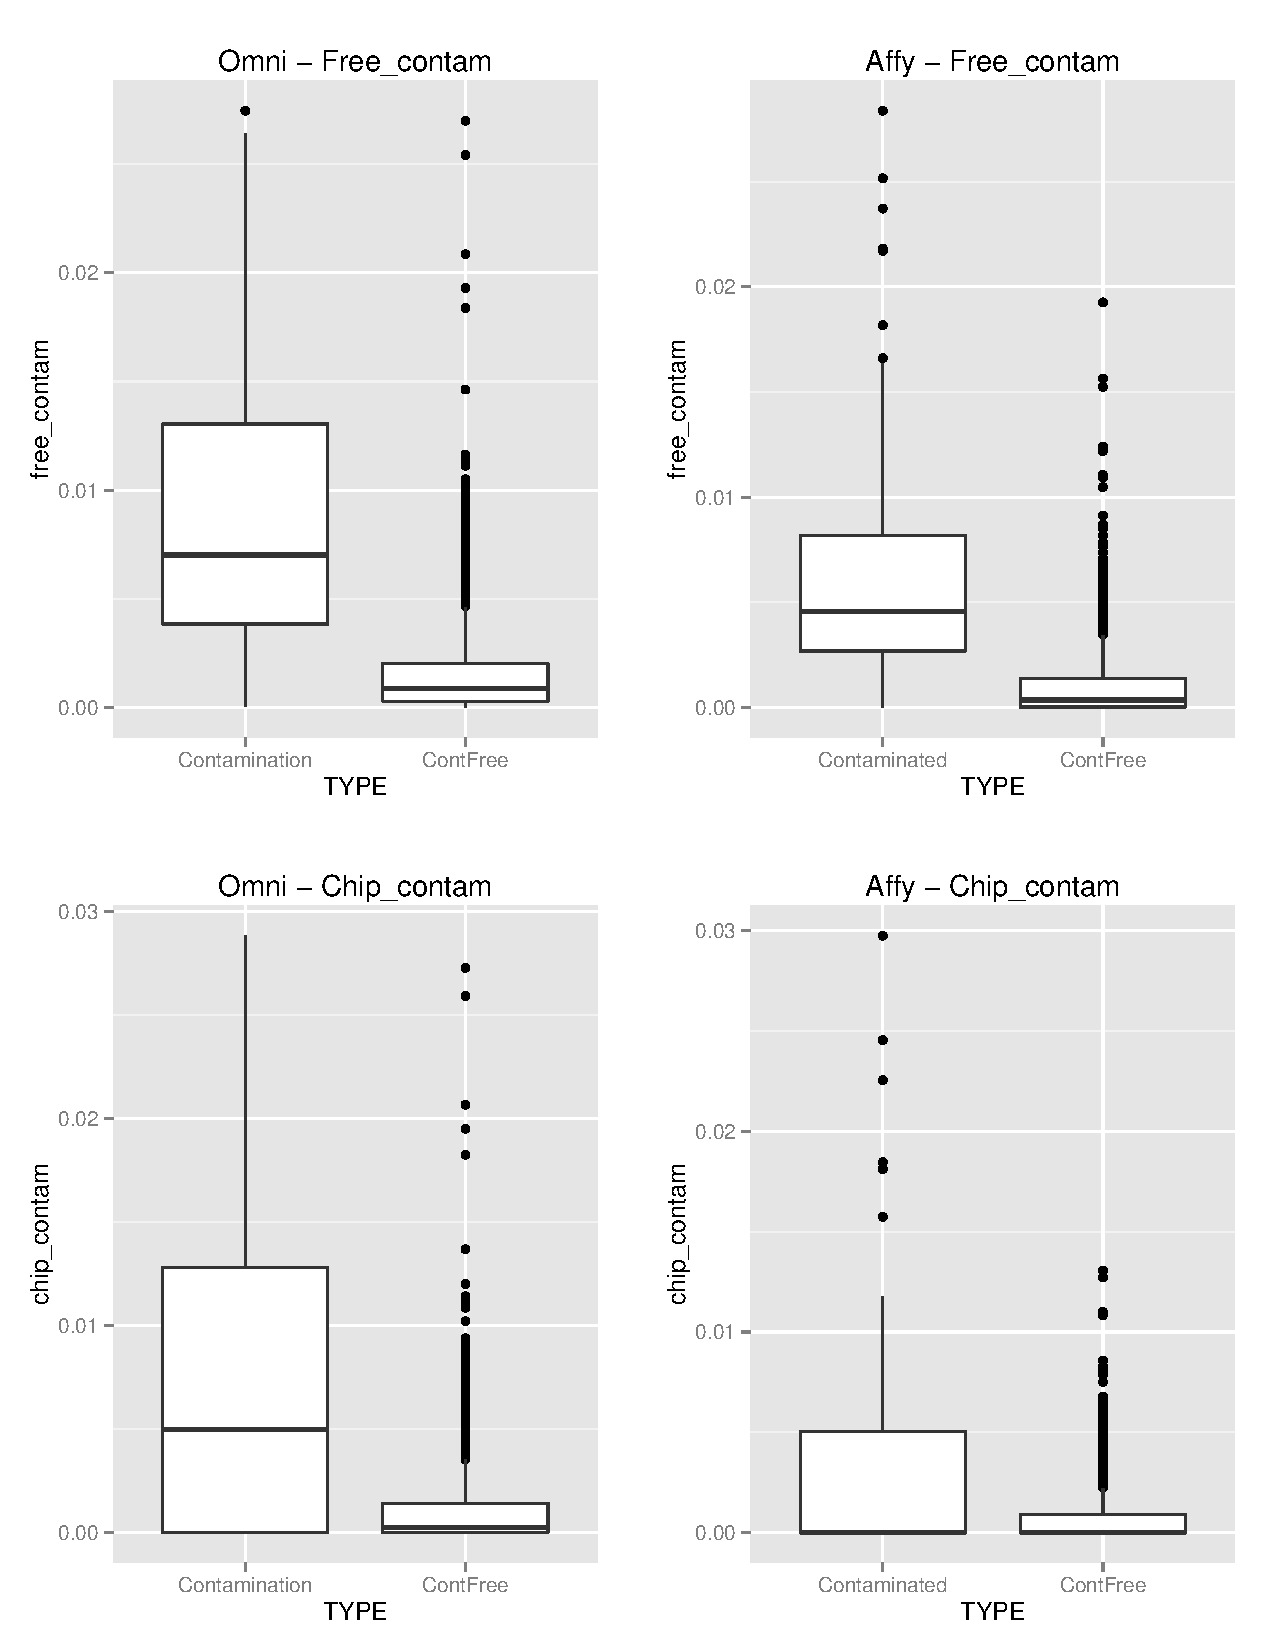
\includegraphics[width=1\textwidth]{images/Result-VerifyBamId-check.pdf}
    \caption[VerifyBamId scores in the contaminated (Contamination) and contamination free (ContFree) Samples]{VerifyBamId scores in the contaminated (Contamination) and contamination free (ContFree) Samples. Omni indicates the scores from VerifyBamId regarding the Illumina Omni Chip, while Affy denotes the Affymetrix Chip scores for VerifyBamId. free\_contam represents the HIGH\_FREE\_MIX, while chip\_contam represents the HIGH\_CHIP\_MIX score}.  
    \label{contScores}
\end{figure}
\end{itemize}

\section{Conclusion and Outlook}\label{cont:outlook}
There are many examples in the literature showing the negative impact of sequencing errors in mtDNA datasets in different areas of research. Standard DNA sequencing procedures are now being replaced by MPS technologies, that are able to retrieve huge amount of sequencing data from biological specimens in a cost-effective manner and short-time span. The arrival of these new technologies is not without problems (\cite{Bandelt2012a}, \cite{Just2015}). The method presented in this Chapter called Haplochecker is a step-forward in the analysis of mtDNA data derived from MPS and it allows preventing sequencing errors and spurious findings. The concept here is to combine the information distilled from the known worldwide phylogeny, based on 24,275 complete humnan mitochondrial DNA sequences\footnote{mtDNA tree Build 17 (18 Feb 2016)\url{http://phylotree.org/}}, providing the database of over 5,400 entries. This database is handled with the JAVA based HaploGrep, by managing the XML-tree directly in memory, read once per instantiation. 

The limitations of the herein presented method are described in Dickins et al \cite{Dickins2014}, but also highlighting the advantage of this approach. The advantage is that contamination can be identified from any source, while already one sample can be analyzed with the entries in the current database, the limitations are identified subsequently:
\begin{itemize}
\item Unavailable haplotypes: This can be indeed of limitation, and the approach here presented highly relies on the data present in the database. There is a clear publication bias in favor to european and asian mtDNA sequences, while african and native american sequences are underrepresented \cite{Fendt2011}. Therefore the limitation will affect merely populations in such branches. 
\item Costly implementation: the authors highlight the relatively costly implementation of a search across a large panel of samples. However we have shown in the Chapter HaploGrep \ref{chapterHaplogrep}, that a query against the in-memory database could be optimized, and the increase of database size follows a linear increase of the run-time. Therefore this limitation is no longer given.
\item Increasing number of haplotypes: the authors argue, that an increase in the number of possible haplotypes and samples increases, leading to a challenging interpretation of the output. As shown with the validation of the 1000G phase 3 dataset, it is also feasible to detect contamination in a set of 2,504 whole genome mtDNA sequences. Projects such as the 100,000 Genome Project\footnote{\url{https://www.genomicsengland.co.uk/the-100000-genomes-project/}} are surely a challenge, but the detection of contamination can be applied also on a per-sample approach, while with the approach of Dickson all sequences need to be in the evaluation, to confirm the contamination, what clearly can be of a challenge in the interpretation of contamination. 
\end{itemize}

While there do exist methods to detect contamination in MPS studies, the herein presented method represents an additional tool for this purpose. Based on various datasets, we could show that the method reliably detects the presence of additional mtDNA profiles, which can be contained to an extent in the 1\% of all reads. 
In addition, it should be denoted, that bioinformatic settings are important for the analysis of high-throughput data and suggest that MPS technologies need further calibration.


\cleardoublepage
\chapter{Discussion and Future Work}
\label{outlook}
\epigraph{Prediction is very difficult, especially about the future.}{\textit{Niels Bohr}}
This thesis presents different software systems for handling mitochondrial genome data derived from various sources, covering the most prominent data formats currently used. This data is generated in high-throughput fashion by either reading the complete genome (e.g. sequencing with NGS) or by inspecting single positions on the DNA (e.g. genotyping with MicroArrays). Especially data derived from NGS devices require preprocessing, to allow the final interpretation of the data, for the detection of variants differing to a reference genome. The amount of data is growing with unprecedented speed, and requires scalable methods for data analysis. This high-throughput also requires additional quality control for sample integrity and reproducible pipelines for generation of valid result reports. Only thereafter the new data generation methods allows uncovering of new findings of origins of mutations and development in various disease. The post-processing of mtDNA data is essential, and bioinformatic tools and parameters influence the final result significantly. 
\section{Discussion}
\label{disc:sec1}
Variants in the mtDNA data, by lacking recombination (there are exception in some species like mussels) remain in linkage disequilibrium \cite{Wallace2013}. Based on this special population genetics property, mtDNA poses its own means of quality control, allowing to group mitochondrial genomes in so called haplogroups. By calculation of haplogroups based on a phylogenetic tree, this thesis describes a scalable algorithm and presents optimizations.  Thereby this tree represents an hypothesis about the evolutionary ancestry of the mitochondrial genome. 

While we developed HaploGrep in summer 2010, several tools for haplogroup classification  have been published, as presented within Chapter \ref{chapterHaplogrep}. The haplogroups are estimated by most of these tools with similar performance \cite{Bandelt2012}, with only a few tools enabling for adequate QC. With growing phylogenetic knowledge, mitochondrial haplogroups increasingly gain importance in investigating the correctness of mitochondrial sequences or genotypes, rendering phylogenetic inference indispensable \cite{weissensteiner2016haplogrep}. The focus of this thesis is on the growing sample sizes in studies, requiring higher speed while simultaneously maintaining accuracy. 
Additional distance metrics were implemented and presented in this regard. By introducing a rule-based engine, covering a set of QCs, an easily to expand system is now implemented in HaploGrep, allowing additional QC. 

HaploGrep 2 is extended for handling data standards, like VCF files or Fasta files. In the first version, our own format HSD was proposed, which is still the most used input format, but a shift towards VCF and Fasta files already started with the publication of the updated version. Thereby the handling of Fasta files is also covered within the rule-based system, since the correct nomenclature can not always be met in an automatic manner.  Although the guidelines for mtDNA typing presented by the DNA Commission of the International Society for Forensic Genetics \cite{Parson2014} were followed, there still can exist ambiguous alignments. Therefore all alignment free derived SNPs are handled differently from SNPs derived from pairwise-alignment, and highlighted as such in the rule-based system.

The handling of mtDNA NGS data requires new methods for the large amount of data generated. Therefore we presented mtDNA-Server, which is a a web server based on Apache Hadoop, by employing the MapReduce paradigm, and splitting the data to smaller chunks to process in parallel manner. It is one tool of many to come, which allows to "democratizing bioinformatics" \footnote{http://www.nature.com/news/how-bioinformatics-tools-are-bringing-genetic-analysis-to-the-masses-1.21545}. By covering aspects from sequence alignment of FASTQ raw data to final results including heteroplasmic variants, all computational tasks in form of tools or pipelines are hidden to the end-user.  Thereby we provide the mtDNA research community an easy to use web server, allowing the detection of heteroplasmic variants in a secure and reproducible way \cite{Weissensteiner2016b}. By validating the integrated heteroplasmy approach, the high sensitivity and specificity of the methods can be shown. mtDNA-Server detects heteroplasmic variants and sample contami- nation accurately, by analyzing artificial sample mix ups, generated in the lab.

As further shown, the haplogroup-based contamination detection in NGS-based sequencing studies, reliably detects sample mix up down to the 1 \% minor allele frequency. 
This within-sample contamination detection has significant general potential to assess data from whole exome or genome sequencing studies for potential contamination and is therefore not limited to target mtDNA sequencing. 

\section{Limitations of current work}
\label{disc:sec2}
Since HaploGrep 2 is based on Phylotree, results are highly dependent on this underlying data. As denoted in the publication, the results should not be accepted blindly. While the results from the haplogroup classification outperform manual classification, warnings and errors highlighted by the rule-based system, need manual inspection. 

As already mentioned in Chapter \cite{chapterHaplogrep}, an automatic generation of the phylogenetic tree is not available, and the manual update is performed every one to two years. This is a limitation not only for population geneticists, but also for the contamination detection, as denoted by Dickins et al.  \cite{Dickins2014}. The concerns here are:
\begin{itemize}
\item if large sets of haplogroups are unknown of limited utility
\item database are needed and integrated with an analysis platform
\item implementation of search across large sample set relatively costly
\item increasing issues with interpretation in large sample size
\end{itemize}
As could be shown in the previous chapter, only the first point here is an actual limitation. The higher the haplogroup resolution, in the underlying tree, the more detailed the contamination detection can be obtained. However phylogenetic method presented in this work, as well as the method by Dickins et al. \cite[Dickins2014] are of limited utility for detecting contamination in family trios or trees with common female ancestors, independently of the haplogroup.

One further limitation of the current work derives from the fact that different reference sequences of mtDNA sequences are in use. While we strictly stick to the rCRS reference sequence, RSRS or the Yoruba reference sequence are not supported directly. mtDNA-Server converts both alternative reference sequences automatically, and annotates the variants according rCRS. While it is straight-forward from the technical view-point to rebuilt the system to work with different reference sequences, it confuses the misunderstandings about reporting mtDNA variation \cite{Bandelt2013}.

\section{Future Work}
\label{disc:sec3}
The data formats presented in Chapter \ref{chap:BioFound} are currently widely accepted, but new data formats are already in use, that requiring to support in the near future. The two most prominent are: the CRAM format and the HDF5 format. The CRAM format specification in the release 3.0\footnote{\url{https://samtools.github.io/hts-specs/CRAMv3.pdf}} describes a lossless compression of SAM files, with better compression compared to BAM and transition between the formats. Special types of the hierarchical data format (HDF5\footnote{\url{https://support.hdfgroup.org/HDF5}}) files are generated by Third-Generation Sequencing devices like the MinION Nanopore, by producing pre-basecalled Fast5 files. The data throughput and data quality increased significantly over the last years, yielding up to 10 Gb per run\footnote{\url{https://nanoporetech.com/about-us/news/human-genome-minion}}. The mtDNA mix-up sample with ratio 1:2 as generated for validation in Chapter \ref{chap:NGS} was already analyzed on this device, by generating single sequences of several Kb length, so that each mitochondrial molecule can now be sequenced at once.

While the presented contamination detection system is available for free as service and  available on GitHub\footnote{\url{https://github.com/haansi/greenVC}}, the HaploGrep source code currently in Apache Subversion (SVN) still needs to be transferred to the GIT version control system, and source code made available to the public. The user interface needs to be updated to a responsive design. The mtDNA-Server is available as service for free as well, and will be made available as Docker Image for local usage, where data is not permitted to be uploaded on our secured server.


\cleardoublepage
\chapter{Conclusion}
\label{chap:conclusion}

\epigraph{One worthwhile task carried to a successful completion is worth a hundred half-finished tasks}{\textit{B.C. Forbes}}

In the last decade, the  field of genomics has moved to a big data science, producing GB of data at decreasing costs, based on the rapid development of new sequencing devices. Subsequently, the bottleneck shifted from data generation to the data analysis, requiring sophisticated methods, in order to derive the most important informations out of the data. Further the high-throughput of the data requires reproducible and scalable pipelines as well as means for quality control. In this thesis an information-system for a small genome, the mitochondrial DNA (mtDNA) is presented, taking the requirements for a pipeline regarding scalability, reproducibility and quality control into account. 

Mitochondrial DNA is coding the most important bioenergetic genes, with mutations involved in a variety of diseases, tumorigenesis and ageing. mtDNA Next-Generation Sequencing (NGS) facilitates detailed insights into mtDNA, enabling to identify new mutations among thousands non-mutated (heteroplasmy) in high resolution. This higher resolution requires additional caution: phantom mutations can become apparent as false positive mutations. A further major issue is the emergence of sample contamination, observable as low level heteroplasmic mutations, leading to deceptive results in medical genetic studies.
This thesis presents our previously developed tools HaploGrep in Chapter \ref{chapterHaplogrep} and mtDNA-Server in Chapter \ref{chap:NGS}, which are merged into a contamination detection system as described in Chapter \ref{chapterContamination}. The two methods are presented, to solve the two main issues:
\begin{itemize}
\item reduce false positive mutations with the help of knowledge distilled from available data sources  
\item detect sample contamination in mtDNA NGS data
\end{itemize}
While HaploGrep automatically classifies the mtDNA profiles to haplogroups with the herein presented algorithms, a further focus is on providing means for mtDNA quality control for detecting issues within those profiles, by introducing a rule-based system. The information in the phylogenetic clusters are shown to allow controls for artificial recombination, phantom mutation, false positive and false negative mutations, as presented within this work. As use case, the data set from the 1000 Genomes Project (n=2,504) was analyzed, by demonstrating the scalability and feasibility of the presented method. While new forms of mitochondrial therapies (like the mitochondrial replacement therapy \cite{Falk2016}) will become more prominent in the near future, haplogroups will become more relevant and an accurate estimation of haplogroups becomes essential. In this regard haplogroup matching is already proposed \cite{Royrvik2016}.

To be able to compare haplogroups based on the mitochondrial profile from a DNA sequence, an alignment step is required, in order to detect the single nucleotide polymorphisms on single bases, as well as insertions or deletions of larger fragments. Different approaches to perform this task are described and an implementation of an hash-index based on k-mers and dynamic programming is presented. The approach is compared to different data structures like suffix arrays and FM-Index, the latter being widely used for Next-Generation Sequencing data, and implemented to run in parallel by adopting JBWA into Cloudgene, as presented in Chapter \ref{chap:NGS}. 

With the previously mentioned progress in data generation by NGS, features of the mtDNA can be researched in more depth, to learn the still poorly understood process of mutation propagation. Here a new concept of processing large amount of mtDNA data derived by massive parallel sequencing devices is presented, by taking advantage of parallel computing architectures based on the MapReduce paradigm. The herein described scalable web server for mtDNA NGS data analysis, directly accepts the raw reads or mapped files from NGS devices without requiring deeper bioinformatic knowledge from the end-user. Thereby the data is processed reference sequence independently and annotated according to the rCRS in highly parallel manner, by employing Apache Hadoop, running on the previously presented Cloudgene framework. Combined with the described maximum likelihood model as well as filter steps like strand-bias score, the workflow provides new insights in low-level mutations, as the result of different sequences per cell or tissue called heteroplasmy. As use-case, again the 1000 Genomes Phase 3 data amounting to $\sim$ 100 GB (from the small mitochondrial genome with 17Kb length) are analyzed. In order to validate the approach, several similar pipelines were compared in terms of sensitivity, specificity and precision. 

Finally the applications described within this work can all be merged into a workflow for detecting contamination in massive parallel sequencing studies. Thereby this approach is based on the concept of haplogroup detection from low-level mutations present in the sequencing data. Different approaches for contamination detection are described and the performance of the approach is evaluated based on the publicly available data-set from the 1000 Genome Consortium, providing 2,504 whole genome sequencing data and sample mix-ups in the lab. We could reliably detect the sample contamination within these data-sets, based on the presented approach.

In conclusion this work presents different algorithms, and implementations that can be applied for a specific task or combined to a system for performing quality control on mtDNA data. Taking advantage of the herein described computational pipeline based on the mtDNA phylogeny, false results as well as sample contamination can be detected as presented. mtDNA being present in whole genome-, whole exome sequencing or RNA-sequencing projects poses the means of an inexpensive and rapid quality control as proposed as part of this work.





\begin{appendix} 
\chapter{Appendix}


%\begin{figure}[!ht]
%    \centering
%    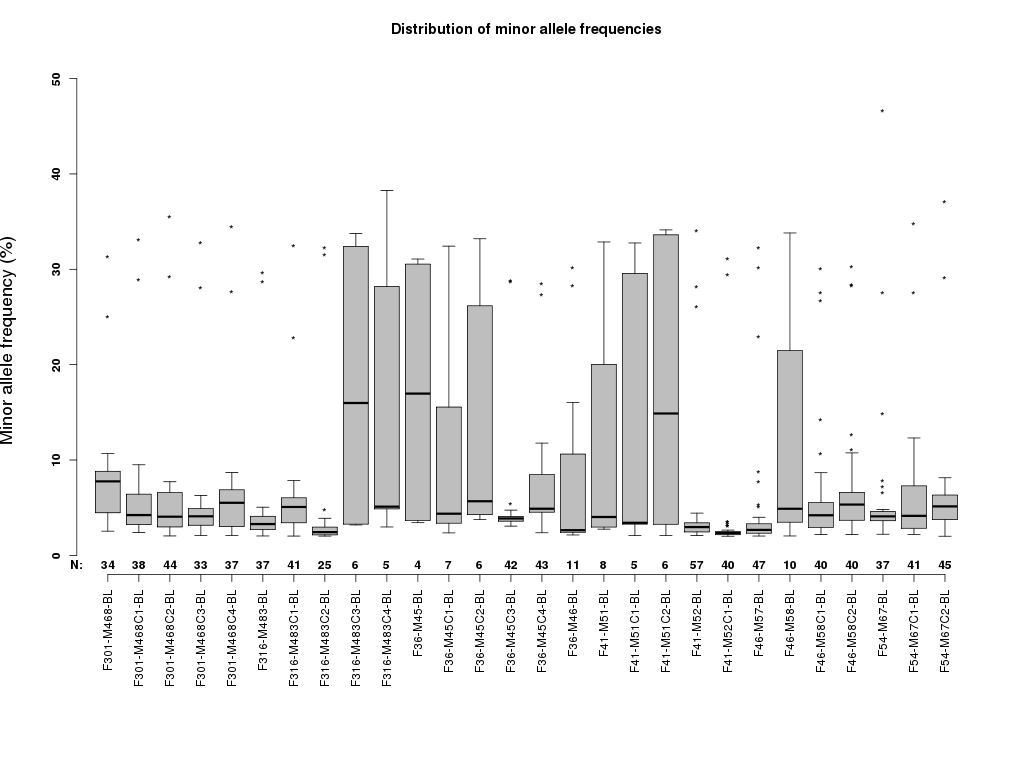
\includegraphics[width=1\textwidth]{images/galaxy-boxplot.png}
%    \caption[Galaxy Boxplot]{Galaxy Boxplot} 
%    \label{app:galaxy-boxplot}
%\end{figure}
The following listing represents the Pipeline for contamination detection defined in Cloudgene 
\begin{lstlisting}[caption={Cloudgene YAML file, defining the HaploChecker Workflow}, label=appyaml]

name: Contamination Check
description:  Check for Contamination
version: 0.1
website: 
category: mtDNA

cluster:

  image: us-east-1/ami-da0cf8b3
  type: m1.large,m1.xlarge
  ports: 80,50030,50070
  creationOnly: false
  installMapred: true
  initScript: install.sh
  service: hadoop
 
mapred:

  steps:
 
    - name: Create HaploGrep Inputfile
      jar: heteroplasmy-check-1.0.jar
      params: --input $input2 --output ${haplogrepInput}.txt

    - name: Haplogroup Contamination Check
      jar: haplogrep.jar
      params: --in ${haplogrepInput}.txt --out ${haplogroupsCheck}.txt --phylotree 16

    - name: Report Creation
      rmd: report.Rmd
      output: ${report}.html
      params: ${haplogroupsCheck}.txt

  inputs:
    - id: input2
      description: Input File
      type: local-folder

  outputs:

    - id: haplogrepInput
      description: Haplogrep Input File
      type: local-file
      download: true

    - id: haplogroupsCheck
      description: Detected Haplogroups Contamination with HaploGrep
      type: local-file
      download: true

    - id: report
      description: Contamination Report
      type: local-file
      download: true 
\end{lstlisting}

% \begin{figure}[!ht]
%     \centering
%     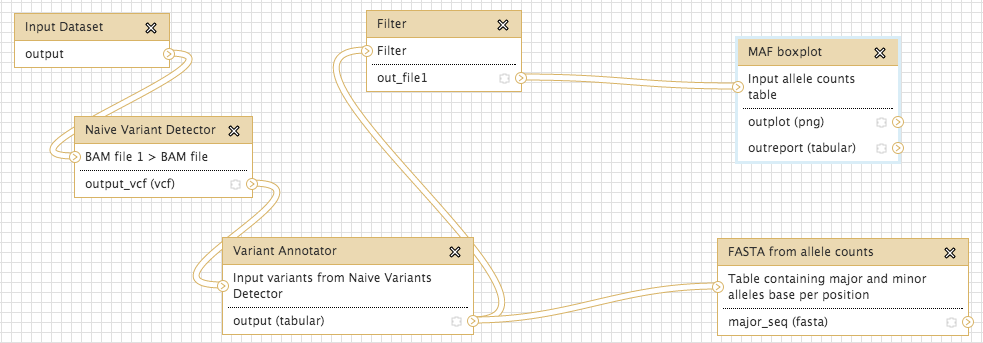
\includegraphics[width=1\textwidth]{images/galaxy-workflow-contamination.png}
%     \caption[Galaxy Workflow for Contamination estimation]{Galaxy Workflow for Contamination estimation} 
%     \label{app:galaxy-workflow}
% \end{figure}


\begin{figure}[!ht]
    \centering
    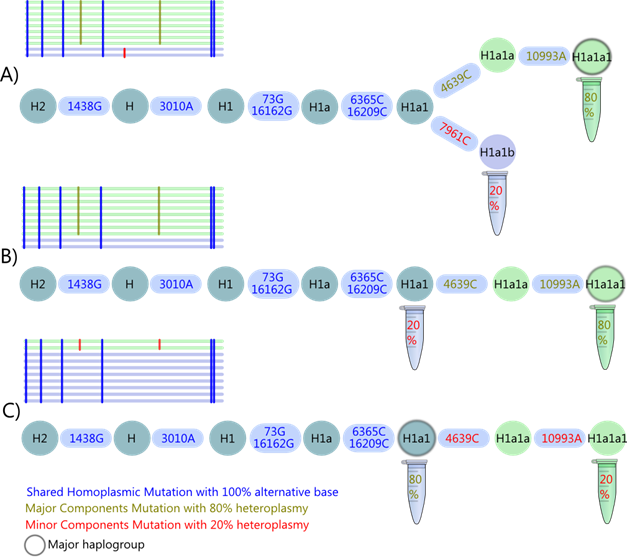
\includegraphics[width=1\textwidth]{images/heteroplasmy.png}
    \caption[Display of all possible pairwise sample contamination]{Display of all possible contaminations by pairwise comparison of major/minor haplotype within one analyzed sample. As an example a contamination level of 20\% over all reads is displayed. Shared polymorphisms of two haplotypes are presented in one branch, whereas the split into diverging branches evidences the two different lineage components (A). A mixture of two haplotypes within a single lineage but of different lineage depths (here minor H1a1 and major H1a1a1) is evidenced if no minor component can be found (B). A mixture of two haplotypes within a single lineage but of different lineage depths (here minor H1a1a1 and major H1a1) is evident if the minor components at equal levels lead to a meaningful haplogroup affiliation (C). Homoplasmic sites facilitate the identification of the branching pattern.} 
    \label{app:galaxy-boxplot}
\end{figure}
\end{appendix}

\listoffigures
\phantomsection  
\addcontentsline{toc}{chapter}{List of Figures}


\cleardoublepage
\phantomsection  

\setstretch{1}

\bibliographystyle{abbrv}
\addcontentsline{toc}{chapter}{Bibliography}
\bibliography{diss}

\cleardoublepage
\phantomsection
\pagestyle{plain}
\addcontentsline{toc}{chapter}{Curriculum Vitae}
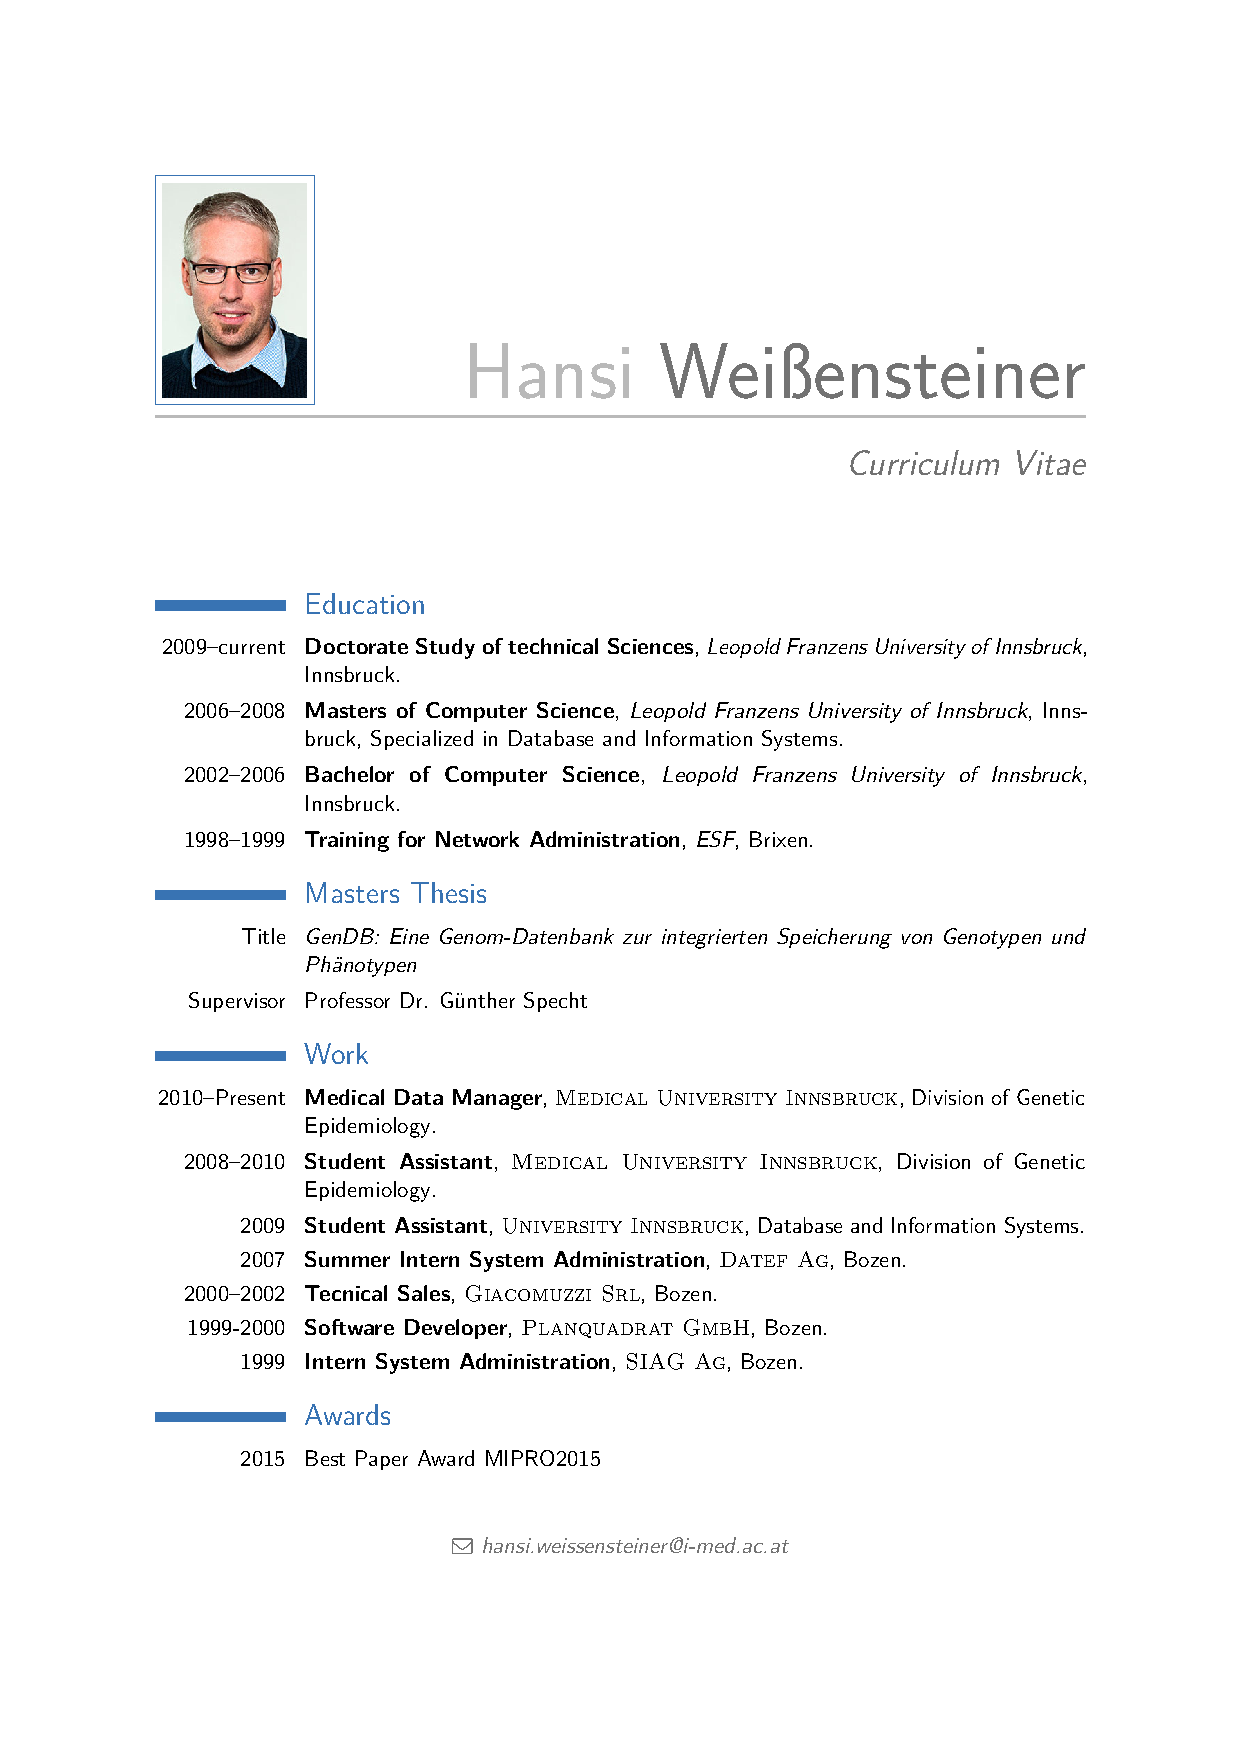
\includepdf[pages=-,pagecommand={}]{CV/hansi.pdf}

\end{document}
